\chapter{Performance Evaluation}
\label{cha:evaluation}
\vspace{0.4 cm}

In this chapter, the proposed system is validated and the performance of the models for the different use cases is evaluated.
The first section presents the datasets provided by MIWenergía\footnote{ \url{https://www.miwenergia.com/} }.
Subsequently, the adopted evaluation methodology is described.
Finally, the evaluation of the performance of the models for the different use cases is presented.
After this chapter, it will be clear how the system has been validated and what the performance achieved by the proposed system is.


\section{MIWenergía datasets}
\label{sec:datasets}
\vspace{0.2 cm}

In this section, the MIWenergía datasets are described.
They provided 3 kinds of datasets: aggregated consumption data from all their customers, consumption data from single customers, and production data from PV plants.

\begin{figure}[H]
\begin{minipage}[b]{8.5cm}
\centering
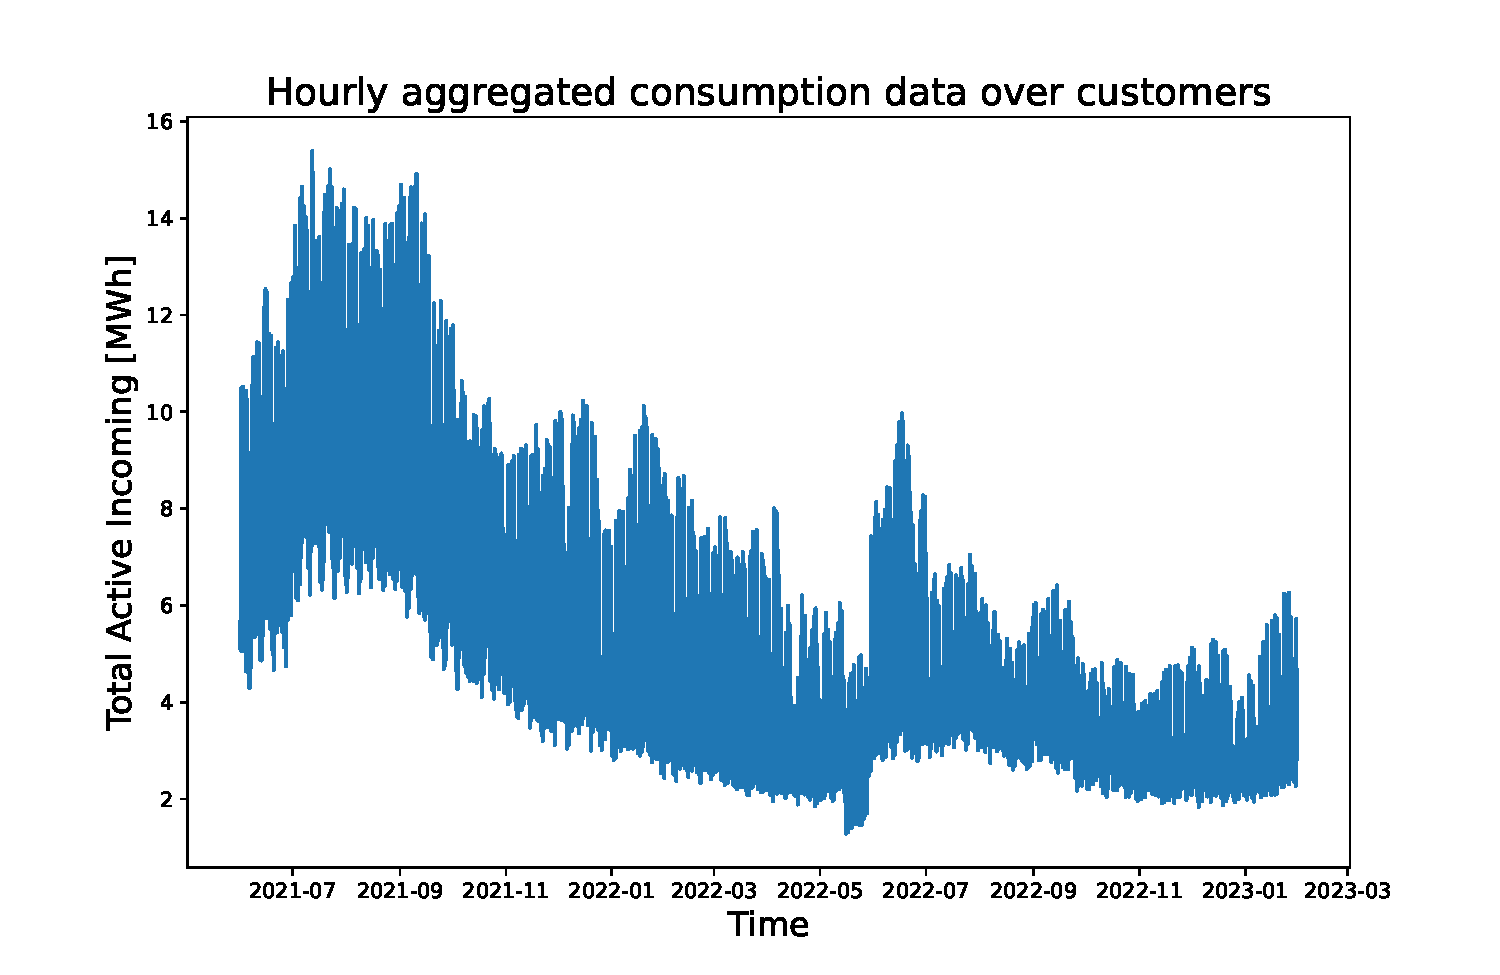
\includegraphics[width=1\textwidth]{images/demand/data_plot}
\subcaption{}
\label{fig:demanddataplot}
\end{minipage}
\ \hspace{2mm} \
\begin{minipage}[b]{8.5cm}
\centering
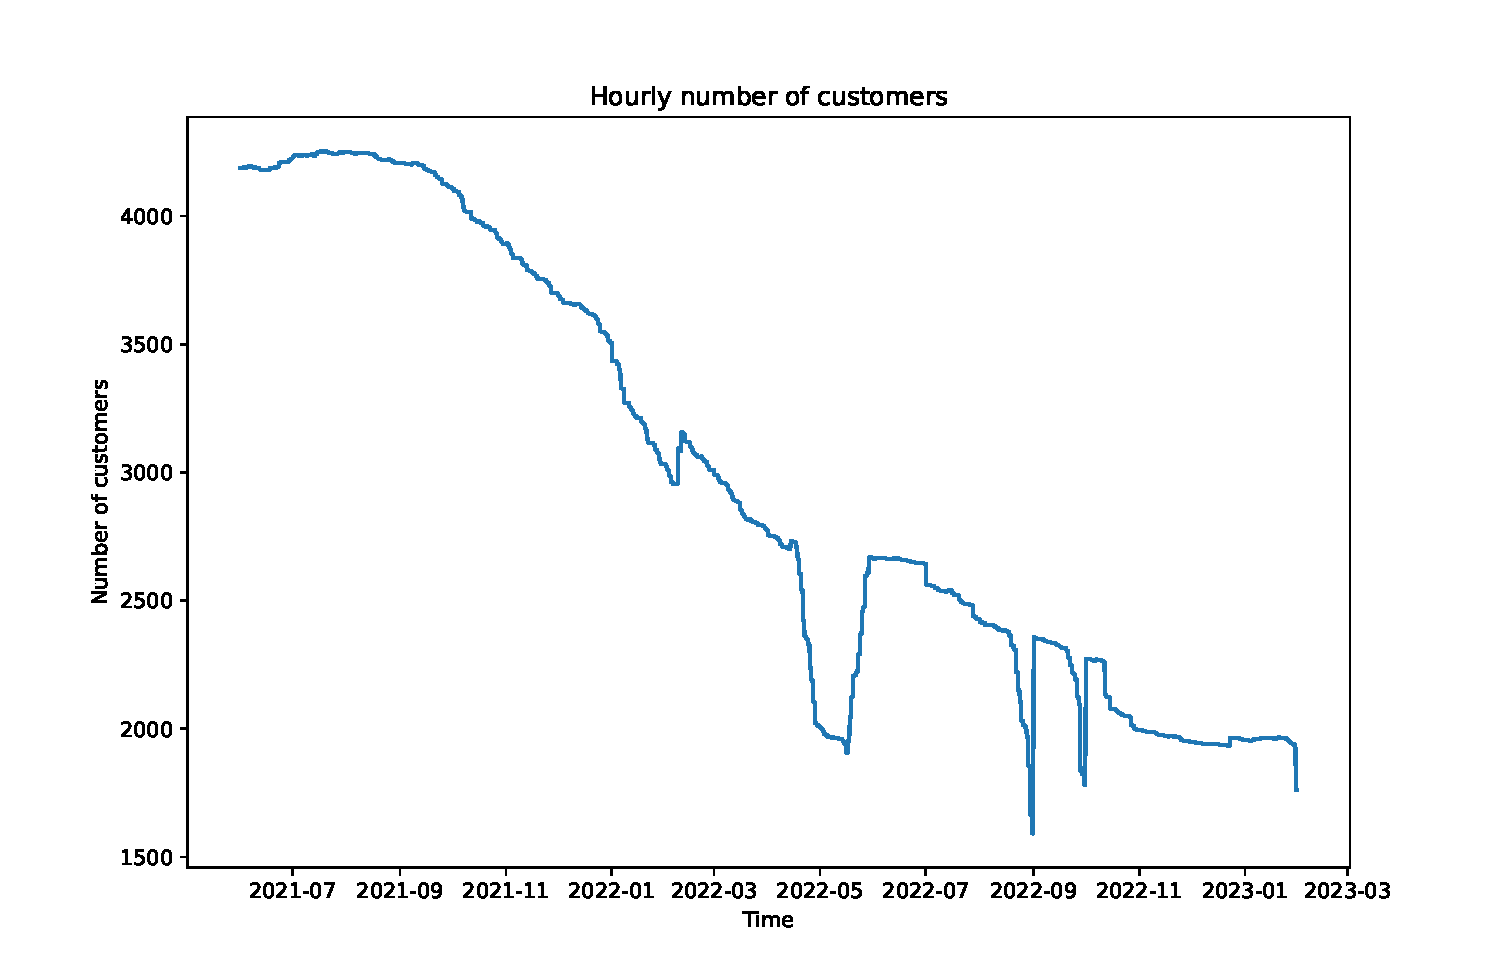
\includegraphics[width=1\textwidth]{images/demand/customers_plot}
\subcaption{}
\label{fig:customersplot}
\end{minipage}
\begin{minipage}[b]{17cm}
\centering
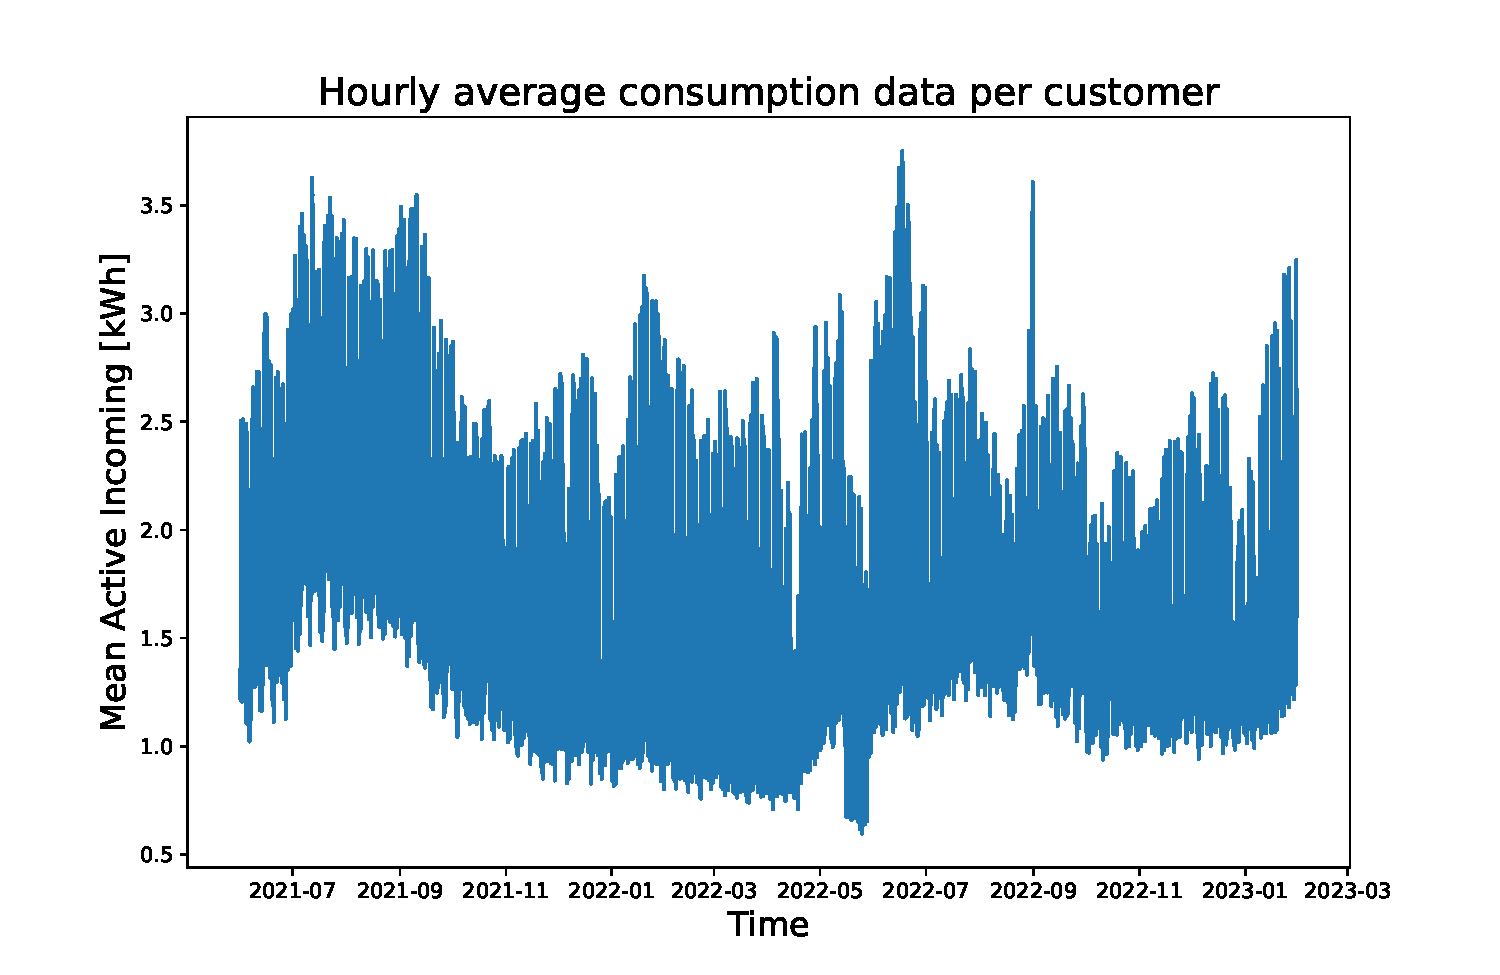
\includegraphics[width=0.5\textwidth]{images/demand/mean_data_plot}
\subcaption{}
\label{fig:meandemanddataplot}
\end{minipage}
\caption{The graphical representation of the hourly \subref{fig:demanddataplot} aggregated consumption over customers, \subref{fig:customersplot} number of customers, and \subref{fig:meandemanddataplot} average consumption per customer.}
\end{figure}

The aggregated consumption data from all their customers consists of hourly aggregated consumption data from June 2021 to January 2023 for a total of 14617 entries.
The graphical representation of the hourly aggregated consumption data is reported in figure~\ref{fig:demanddataplot}.
The number of customers is variable, with a maximum of 4253, a minimum of 1591, a mean of 2988, and a standard deviation of 855.
The graphical representation of the hourly number of customers is reported in figure~\ref{fig:customersplot}.
It was thought to normalize the consumption on the basis of the number of customers in order to study the average consumption per user, as illustrated in figure~\ref{fig:meandemanddataplot}, and then multiply by the number of customers.
However, this was not feasible since often this value changes significantly without reflecting on the consumption data, this information was deemed unreliable and not utilized.
Despite this limitation, the average consumption per customer still provided valuable insights into consumption patterns.
Specifically, it suggested the presence of two consumption peaks: one in the summer, likely attributed to air conditioning systems, and a second peak in the winter, likely caused by heating systems.

The consumption data from single customers consists of hourly aggregated consumption data of three customers:
\begin{enumerate}
  \item from June 2021 to August 2022 for a total of 10952 total entries and it is represented in figure~\ref{fig:dataplotcustomer1};
  \item from September 2021 to May 2022 for a total of 5855 total entries and it is represented in figure~\ref{fig:dataplotcustomer2};
  \item from September 2021 to August 2022 for a total of 8760 total entries and it is represented in figure~\ref{fig:dataplotcustomer3}.
\end{enumerate}
The total entries for the three customers are 25567 in the overall period from June 2021 to August 2022.

\begin{figure}[H]
\begin{minipage}[b]{8.5cm}
\centering
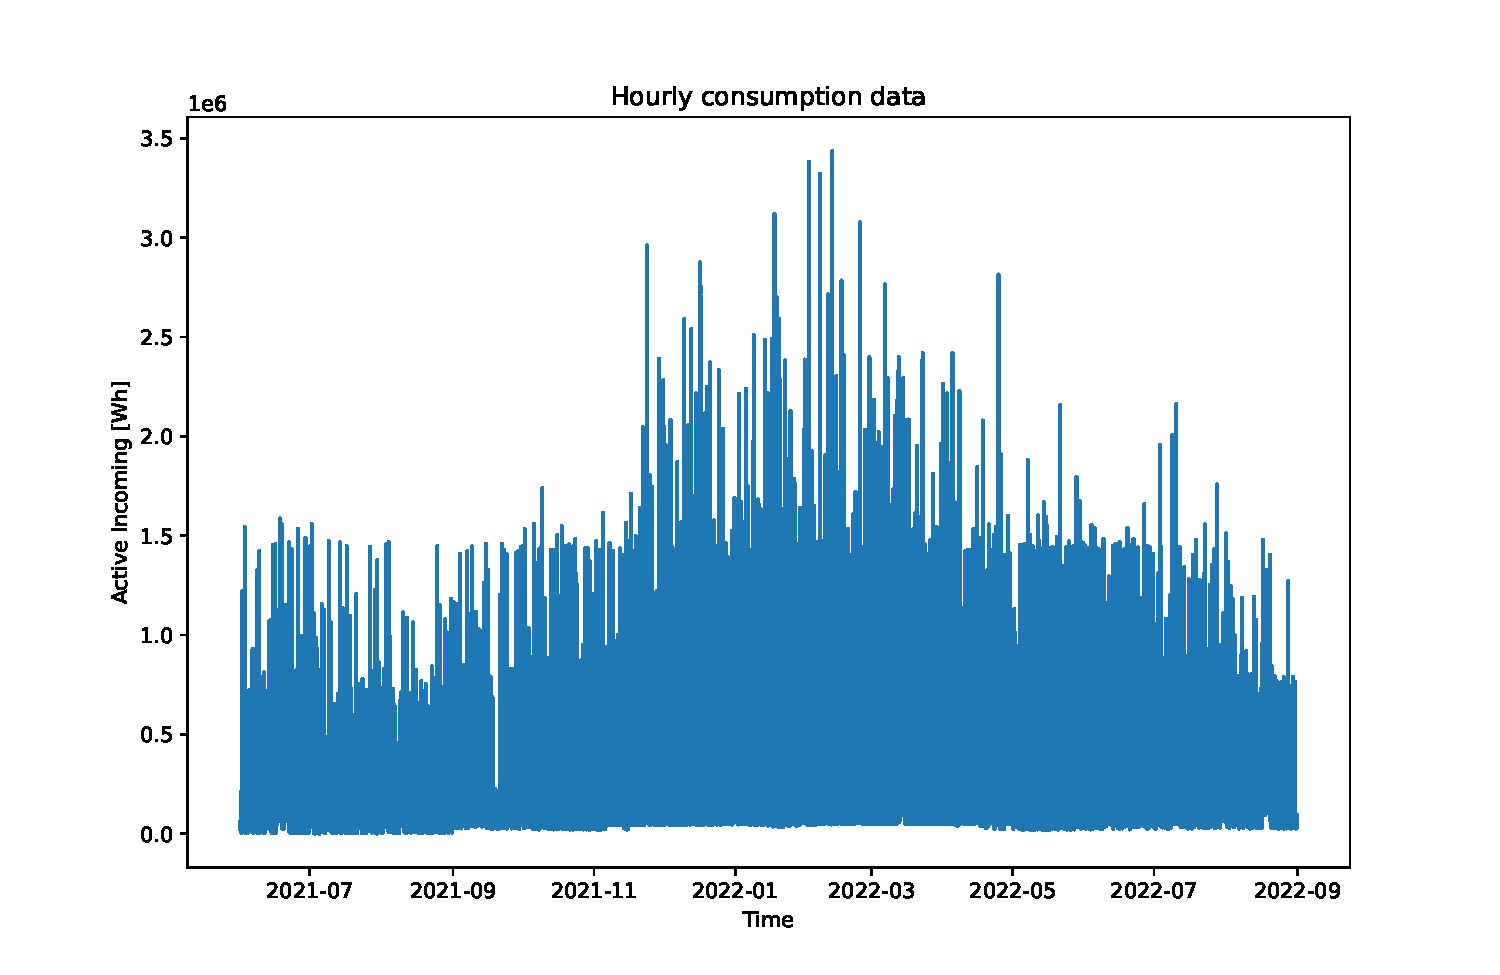
\includegraphics[width=1\textwidth]{images/baseline/data_plot_customer1}
\subcaption{First customer.}
\label{fig:dataplotcustomer1}
\end{minipage}
\ \hspace{2mm} \
\begin{minipage}[b]{8.5cm}
\centering
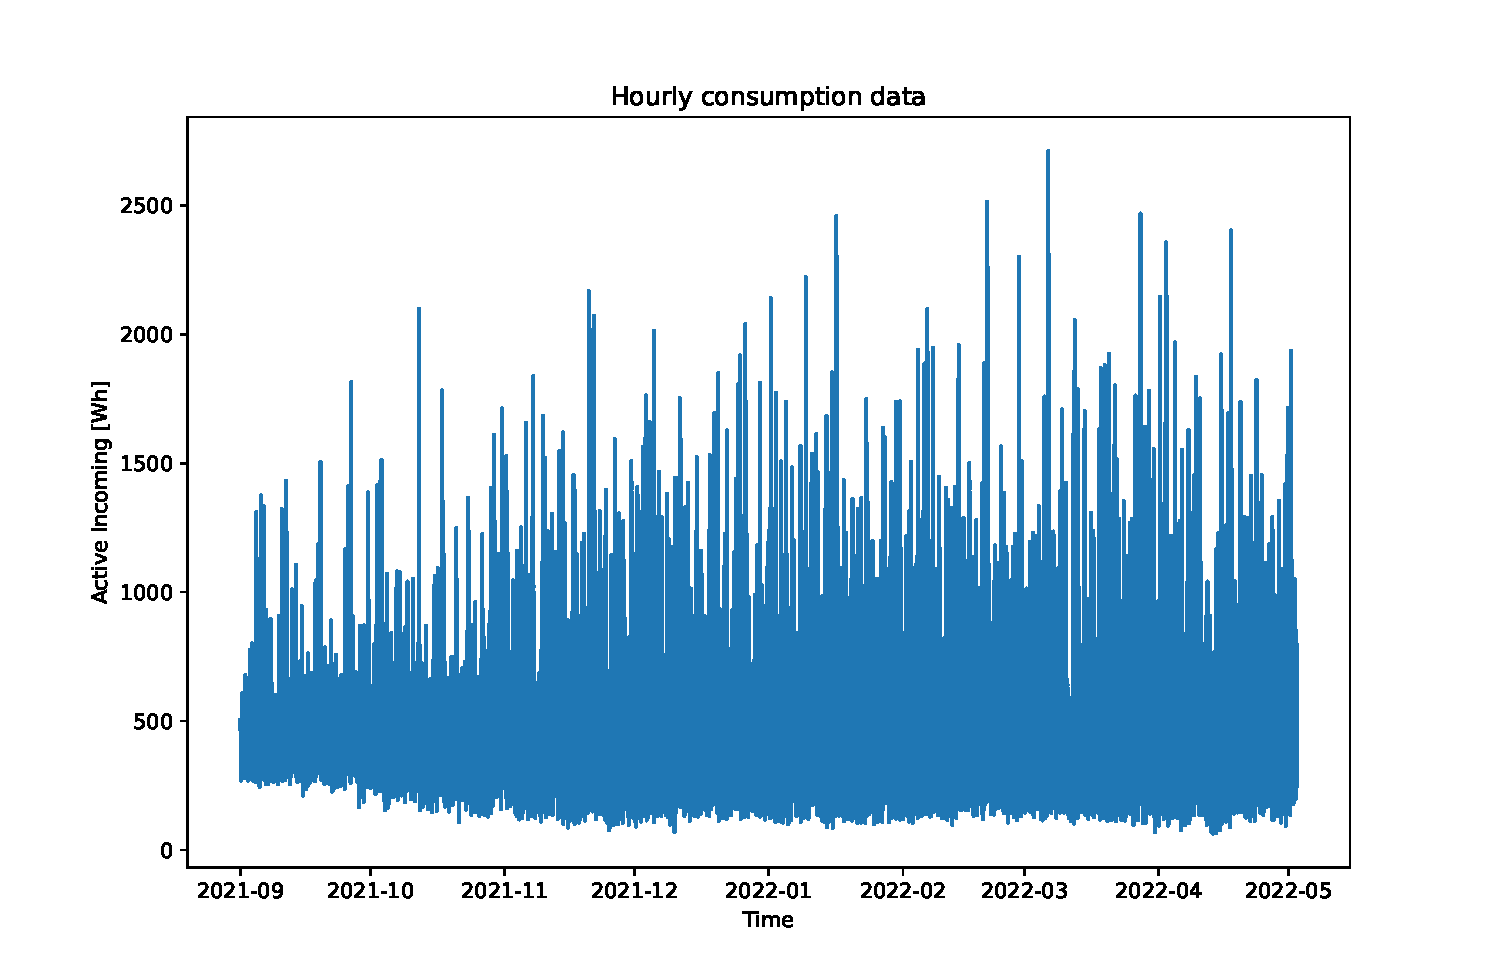
\includegraphics[width=1\textwidth]{images/baseline/data_plot_customer2}
\subcaption{Second customer.}
\label{fig:dataplotcustomer2}
\end{minipage}
\begin{minipage}[b]{17cm}
\centering
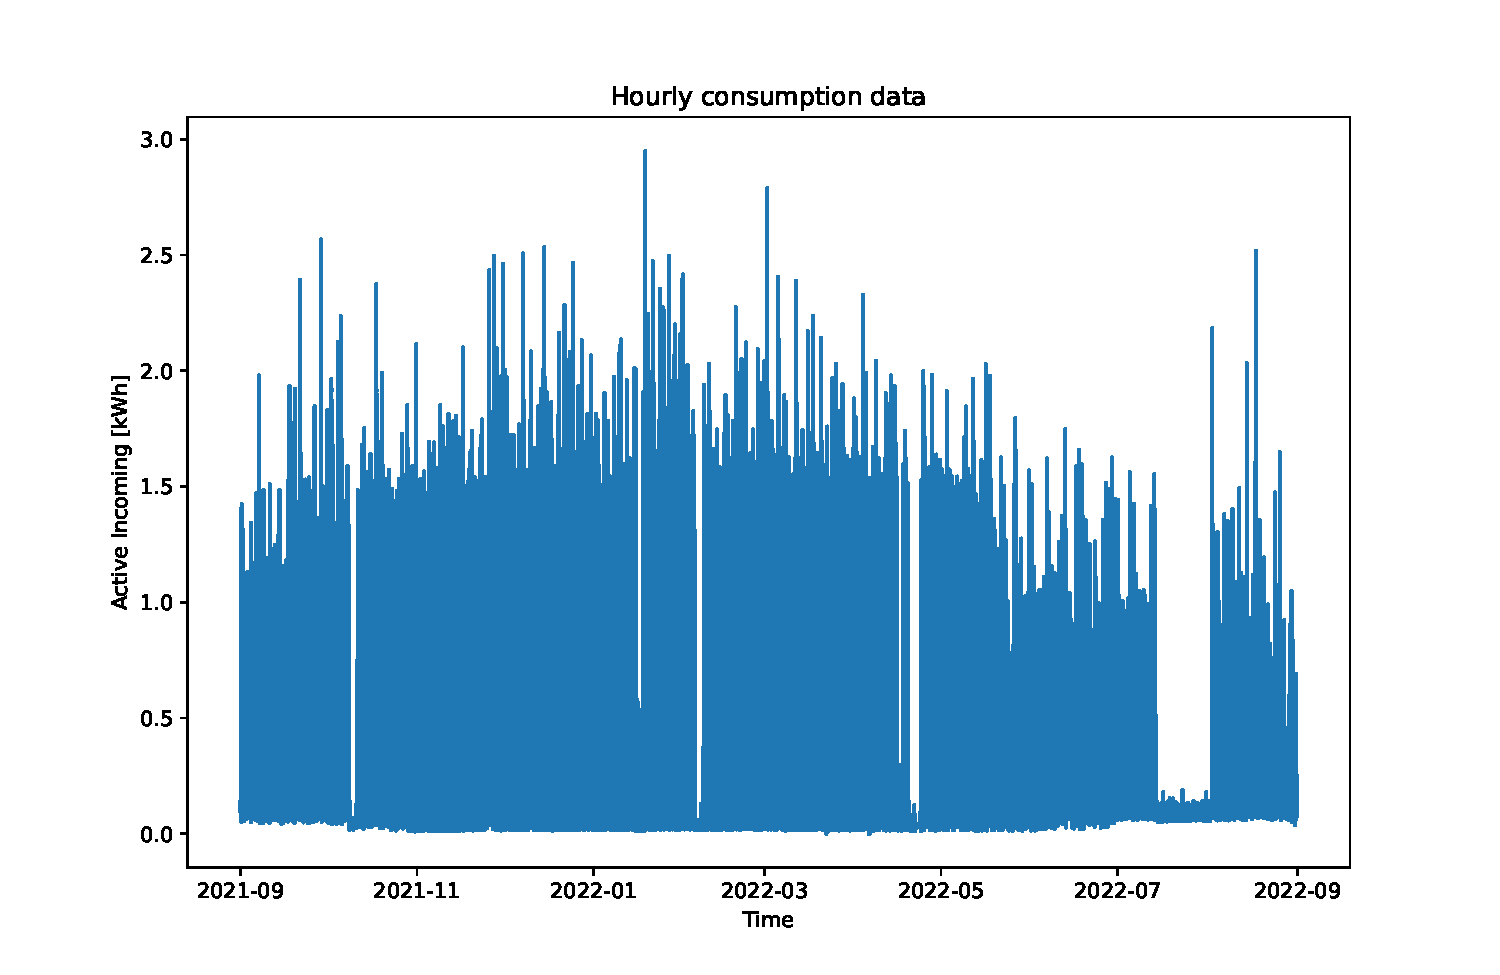
\includegraphics[width=0.5\textwidth]{images/baseline/data_plot_customer3}
\subcaption{Third customer.}
\label{fig:dataplotcustomer3}
\end{minipage}
\caption{The graphical representation of the consumption data of the three customers.}
\end{figure}

Only consumption data for three customers were provided, as electricity consumption data of customers is considered personal data as stated in the Directive (EU) 2019/944 of the European Parliament\footnote{ \url{https://eur-lex.europa.eu/legal-content/EN/TXT/?uri=CELEX:32019L0944} }, which establishes common rules for the internal market for electricity.
As such, the data falls under the scope of the General Data Protection Regulation (GDPR)\footnote{ \url{https://gdpr-info.eu/} }, which requires explicit consent for processing personal data.
Therefore, it is likely that the provided data came from MIWenergía's internal employees who consented to participate in the research.
In fact, the provided data were needed for a technical feasibility study.
However, to identify consumption patterns among a broader population, data from more customers would be required.

By analyzing the data plots, it can be observed that the consumption patterns of the three customers are quite distinct.
For instance:
\begin{itemize}
  \item The first customer's consumption is consistently below 1.5 kWh throughout the year except for the winter season;
  \item The second customer shows almost the same consumption pattern;
  \item The third customer has a dense series with some gaps with very low consumption in parts of the year, probably due to time periods away from home.
\end{itemize}

The production data from 8 PV plants consists of hourly aggregated production data:
\begin{enumerate}
  \item from January 2022 to October 2022 for a total of 7296 total entries and it has a nominal power of 149.75 kW;
  \item from February 2022 to October 2022 for a total of 6552 total entries and it has a nominal power of 237.6 kW;
  \item from February 2022 to October 2022 for a total of 6552 total entries and it has a nominal power of 158.4 kW;
  \item from June 2022 to October 2022 for a total of 3576 total entries and it has a nominal power of 1240 kW;
  \item from September 2022 to October 2022 for a total of 1465 total entries and it has a nominal power of 126.2 kW;
  \item from September 2022 to October 2022 for a total of 1465 total entries and it has a nominal power of 113 kW;
  \item from September 2022 to October 2022 for a total of 1465 total entries and it has a nominal power of 45 kW;
  \item from September 2022 to October 2022 for a total of 1465 total entries and it has a nominal power of 100 kW;
\end{enumerate}
The total entries for the 8 PV plants are 29836 total entries in the overall period from January 2022 to October 2022, aggregating over plants the resulting entries are 7296.
The graphical representation of the hourly aggregated total and mean percentage production data are reported respectively in figure~\ref{fig:productiondataplot} and figure~\ref{fig:productiondataplotpercentage}.

The same weather data from the same provider and the same weather station were used for all the tasks.
While it is reasonable to assume that some weather conditions, such as clouds, may vary and affect consumption and production differently, this approach was taken since the customers and the PV plants were in the same area, with a maximum distance of around 100 km between them, and also because the value of the weather parameters is an average of the values recorded in the past hour.
Therefore, using the same weather data is deemed appropriate for the analysis at hand, given that it reflects the weather conditions in the area over a broad time frame.

\begin{figure}[H]
\begin{minipage}[b]{8.5cm}
\centering
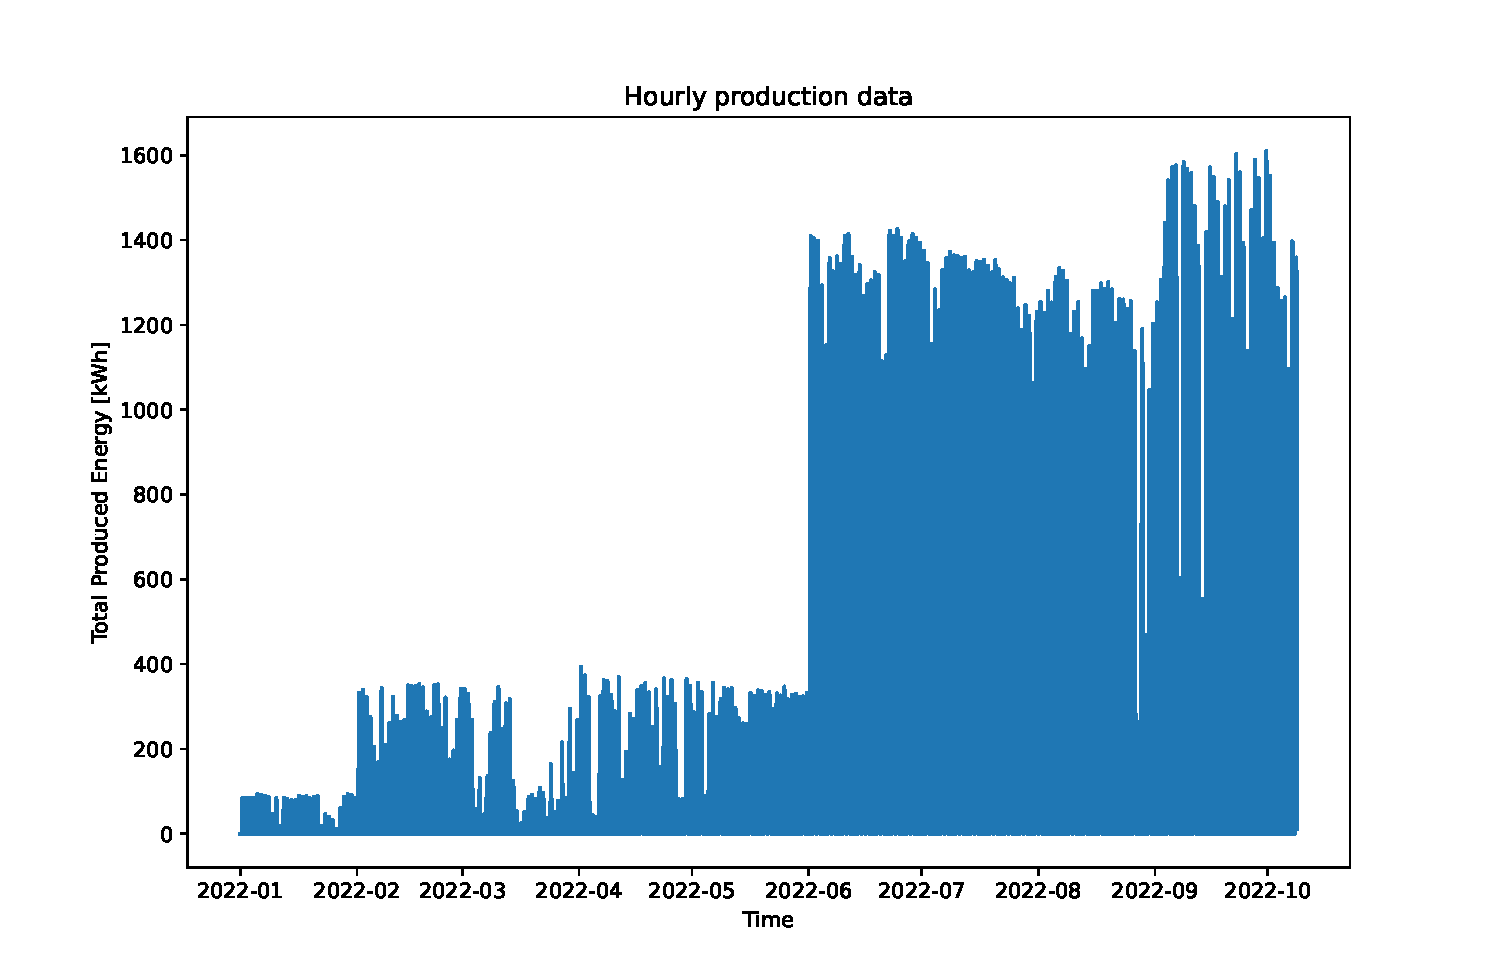
\includegraphics[width=1\textwidth]{images/production/data_plot}
\subcaption{}
\label{fig:productiondataplot}
\end{minipage}
\ \hspace{2mm} \
\begin{minipage}[b]{8.5cm}
\centering
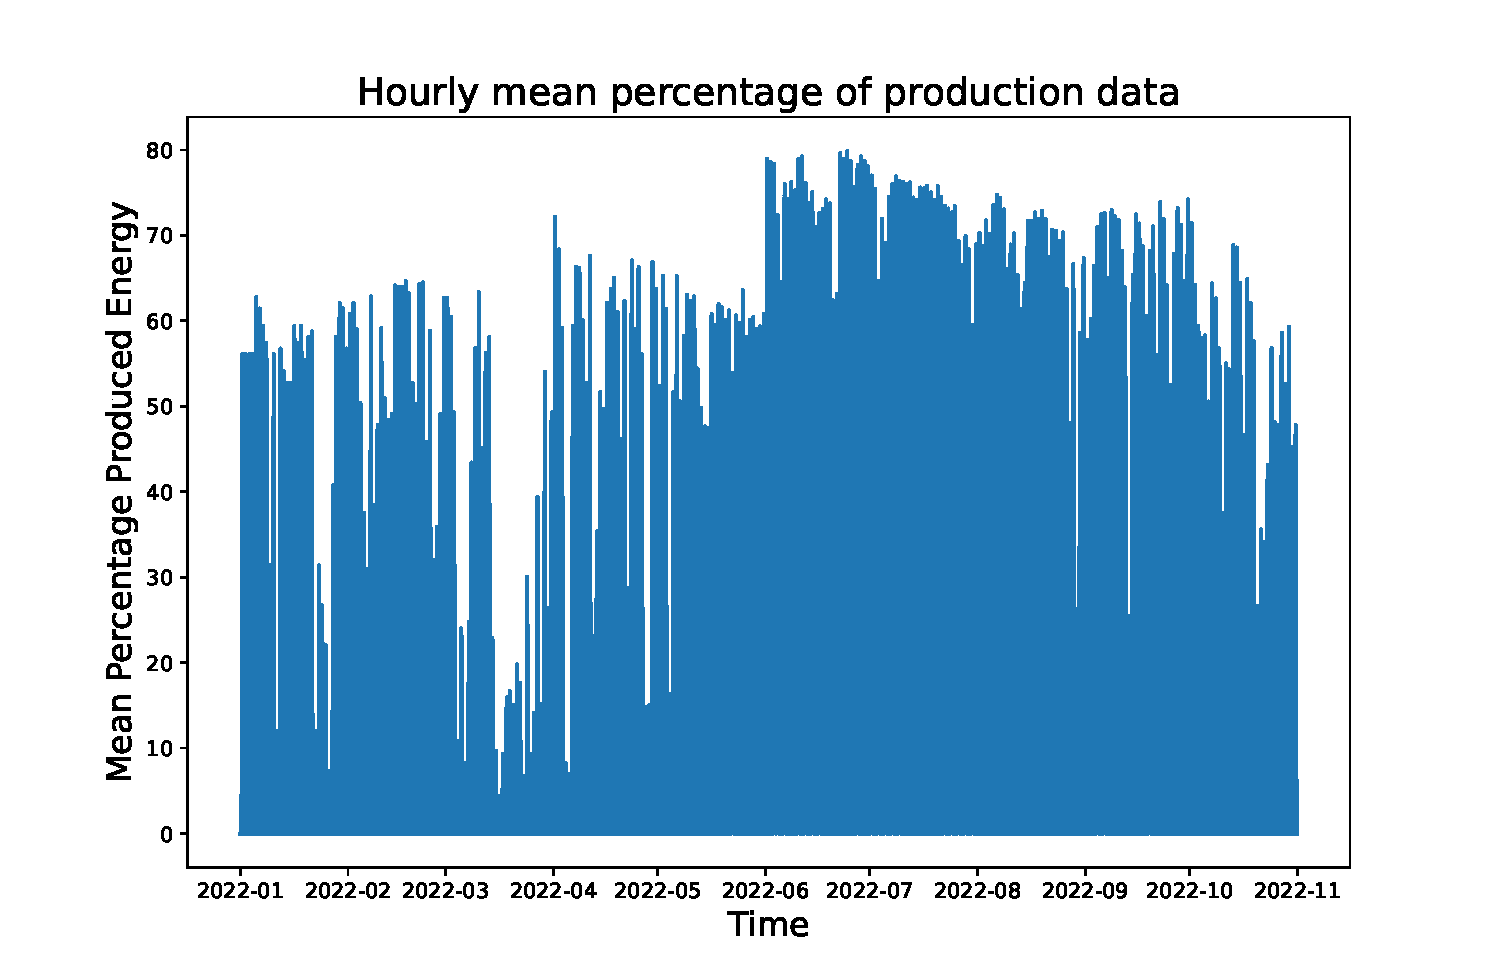
\includegraphics[width=1\textwidth]{images/production/data_plot_percentage}
\subcaption{}
\label{fig:productiondataplotpercentage}
\end{minipage}
\caption{The graphical representation of the hourly aggregated \subref{fig:productiondataplot} total and \subref{fig:productiondataplotpercentage} mean percentage production data.}
\end{figure}


\section{Evaluation methodology}
\label{sec:methodology}
\vspace{0.2 cm}

The evaluation methodology was based on two relevant error metrics: Mean Absolute Percentage Error (MAPE) and Mean Absolute Error (MAE).
These are standard and widely used metrics in time series forecasting for different use cases, as reported in many articles and books such as \cite{armstrong2001principles, DEGOOIJER2006443, HYNDMAN2006679}.
The MAPE is defined as $\text{MAPE}(y, \hat{y}) = \frac{100\%}{N} \sum_{i=0}^{N - 1} \frac{|y_i - \hat{y}_i|}{|y_i|}$.
It is the most relevant error metric for all the tasks since it is a percentage-based error metric that takes into account the magnitude of the errors relative to the actual values.
The MAE is defined as $\text{MAE}(y, \hat{y}) = \frac{ \sum_{i=0}^{N - 1} |y_i - \hat{y}_i| }{N}$.
It is the most suitable error metric in consumption baseline forecasting where there is a high variability from very low to high values, and electricity production forecasting where there is a significant number of zeros when the sun is absent.

\begin{figure}[H]
\centering
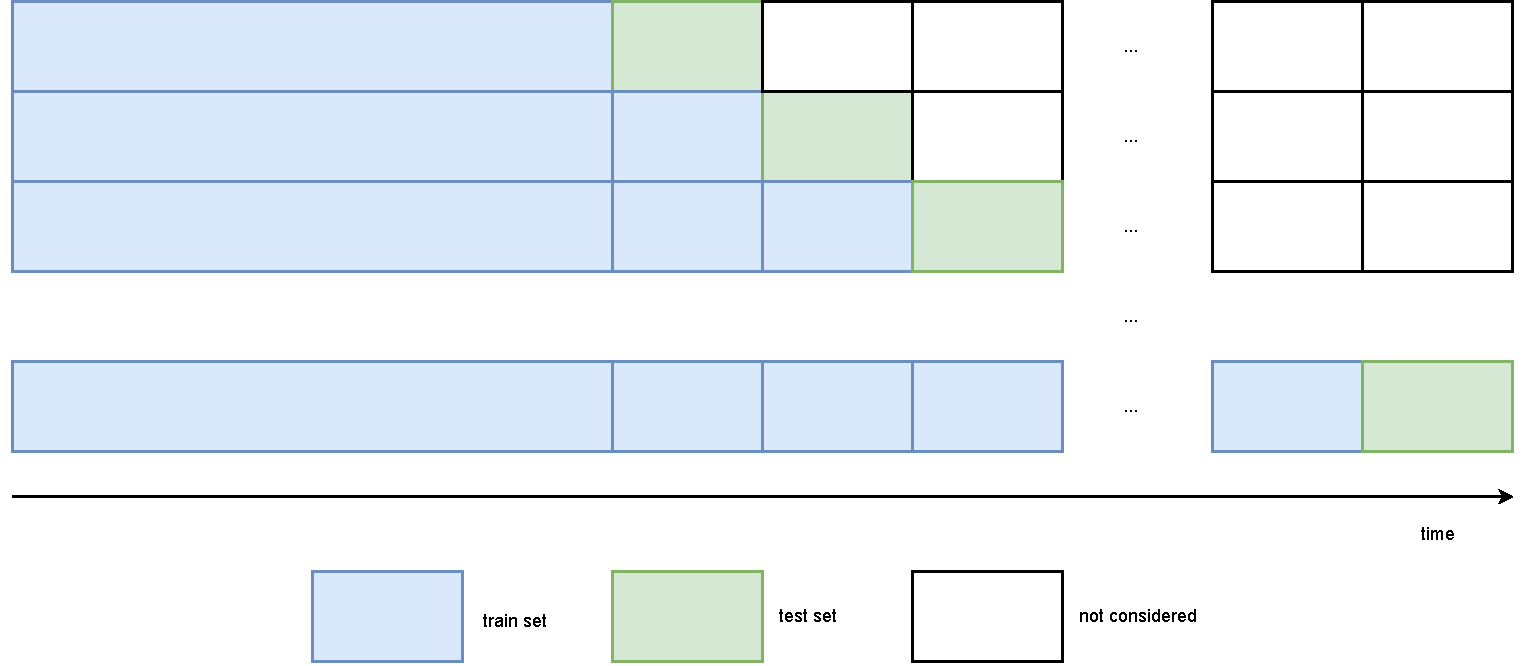
\includegraphics[width=0.8\textwidth]{images/cross_validation}
\caption{The schematic representation of the blocked k-fold cross-validation adopted.}
\label{fig:crossvalidation}
\end{figure}

For assessing the model performance when dealing with time series data, the traditional cross-validation techniques are not suitable as they assume that the data points are independent and identically distributed (i.i.d.), which is not the case in time series data, as also reported in the chapter~\ref{cha:soa} by the following articles \cite{BERGMEIR2012192, Cerqueira2020}.
In fact, in time series data the order of the observations matters, and there are temporal dependencies between the observations.
Therefore, a more appropriate technique for evaluating time series models is blocked k-fold cross-validation.
The basic idea of blocked k-fold cross-validation is to split the data considering multiple training and test sets, where the training set only includes data from the past and the test set includes data from the future.
This simulates the real-world scenario where we want to make predictions about the future based on past data.
In figure~\ref{fig:crossvalidation}, the schematic representation of how the blocked k-fold cross-validation was performed is reported, 12 splits were used with a test size depending on the specific use case.
The training set is increased by adding the previous test elements at every successive evaluation.

Another technique, reported in \cite{Cerqueira2020} is the repeated holdout approach repeated in multiple testing periods using a Monte Carlo simulation.
This approach involved using 70\% of the total observations of the time series in each test.
For each period, a random point from the time series was selected, and a training window comprising 60\% of the time series before the selected point was used for training, while a testing window of 10\% of the time series after the selected point was used for evaluation.
In the paper, it was stated that the approach provided the most accurate estimates when the time series are non-stationary.
However, for having the same evaluation mechanisms on all the models and simulating the fact that the model starts with limited data and then the training amount increases over time to obtain better performance, block validation was used using the TimeSeriesSplit provided by the scikit-learn library.
Moreover, the considered data are without a strong trend as reported in the dedicated sections of the specific use cases where the data and the model forecasts are analyzed.

In addition to the blocked k-fold cross-validation results also the results on the last test split using the rest as training are reported.
This was done since it provides insight on which could be the performance of the models in forecasting the near future data with the currently available training data.
A table summarizing the metrics and the evaluation mechanisms adopted for the use cases is reported in table~\ref{tab:metricstable}.

\begin{table}[H]
\centering
\begin{tabular}{|c|c|c|}
\hline
\textbf{Use case} & \textbf{Metrics} & \textbf{Evaluation mechanisms}\\
\hline
Electricity demand & MAPE & blocked k-fold cross-validation\\
forecasting & & and test on the last split\\
\hline
Electricity production & MAE & blocked k-fold cross-validation\\
forecasting & & and test on the last split\\
\hline
Consumption baseline & MAPE and MAE & blocked k-fold cross-validation\\
forecasting & & and test on the last split\\
\hline
\end{tabular}
\caption{Table summarizing the metrics and the evaluation mechanisms adopted for the use cases.}
\label{tab:metricstable}
\end{table}

This evaluation methodology was used at training time to study the performance over time.
At forecasting time, the performance on the last time slot was treated with more attention as the most relevant for the energy retailers since the most related to the performance on imminent future data.
The combinations of the models were done just at forecasting time on the last time slot using the average of some approaches for studying whether there could be a beneficial effect on the forecasts and compensation of error between the different approaches.
The same was also done for the AutoML approach, in fact, it was tested just at forecasting time on the last time slot for comparison to the tested models.
It was included as a baseline to show how a general-purpose framework can perform in specific use cases compared to specific architectures designed for the task.

As explained in chapter~\ref{cha:implementation}, for all the use cases, there is a difference between training and forecasting time for the ML (support vector regressor, hist gradient boosting regressor, and extreme gradient boosting regressor) and DL (LSTM, GRU, and CNN) models.
In particular, for these models, a recursive strategy to generate multi-step forecasts was adopted.
This approach is a standard classical technique covered in various textbooks, including \cite{Manu2022}.
It offers advantages such as simplicity in understanding, clear temporal dependency as previous forecasts are used as input for subsequent ones, flexibility to be applied to different models, and adaptability to various forecasting horizons, which is crucial when integrating it into a SaaS solution.
However, there are also disadvantages associated with this approach.
Error propagation can occur, and this can be observed in the forecasting results, where small inaccuracies in initial predictions can accumulate and lead to larger errors over time.
Sub-optimality is another drawback, as the optimality achieved for one-step forecasting may not generalize well to multi-step forecasting.
Additionally, the computational complexity is high as the model needs to be run for each individual step.
In contrast, the other approaches: baselines, ARIMA/SARIMA, Prophet, and TFT directly handle the concept of multi-step prediction and present no difference between training and forecasting time.


\section{Electricity demand forecasting}
\label{sec:demandval}
\vspace{0.2 cm}

The aggregated consumption data over the customers is analyzed to get some descriptive analytics before finding adequate models to forecast the demand.
The time series decomposition using an additive model of the hourly aggregated consumption over the customers considering as period of the time series a week is reported in figure~\ref{fig:demanddecomposition}.
It showed a considerable amount of noise, comparable to seasonality in magnitude.
The trend showed 2 peaks during the summer season, the first being more emphasized since it also corresponds to a peak in the number of users.

\begin{figure}[H]
\centering
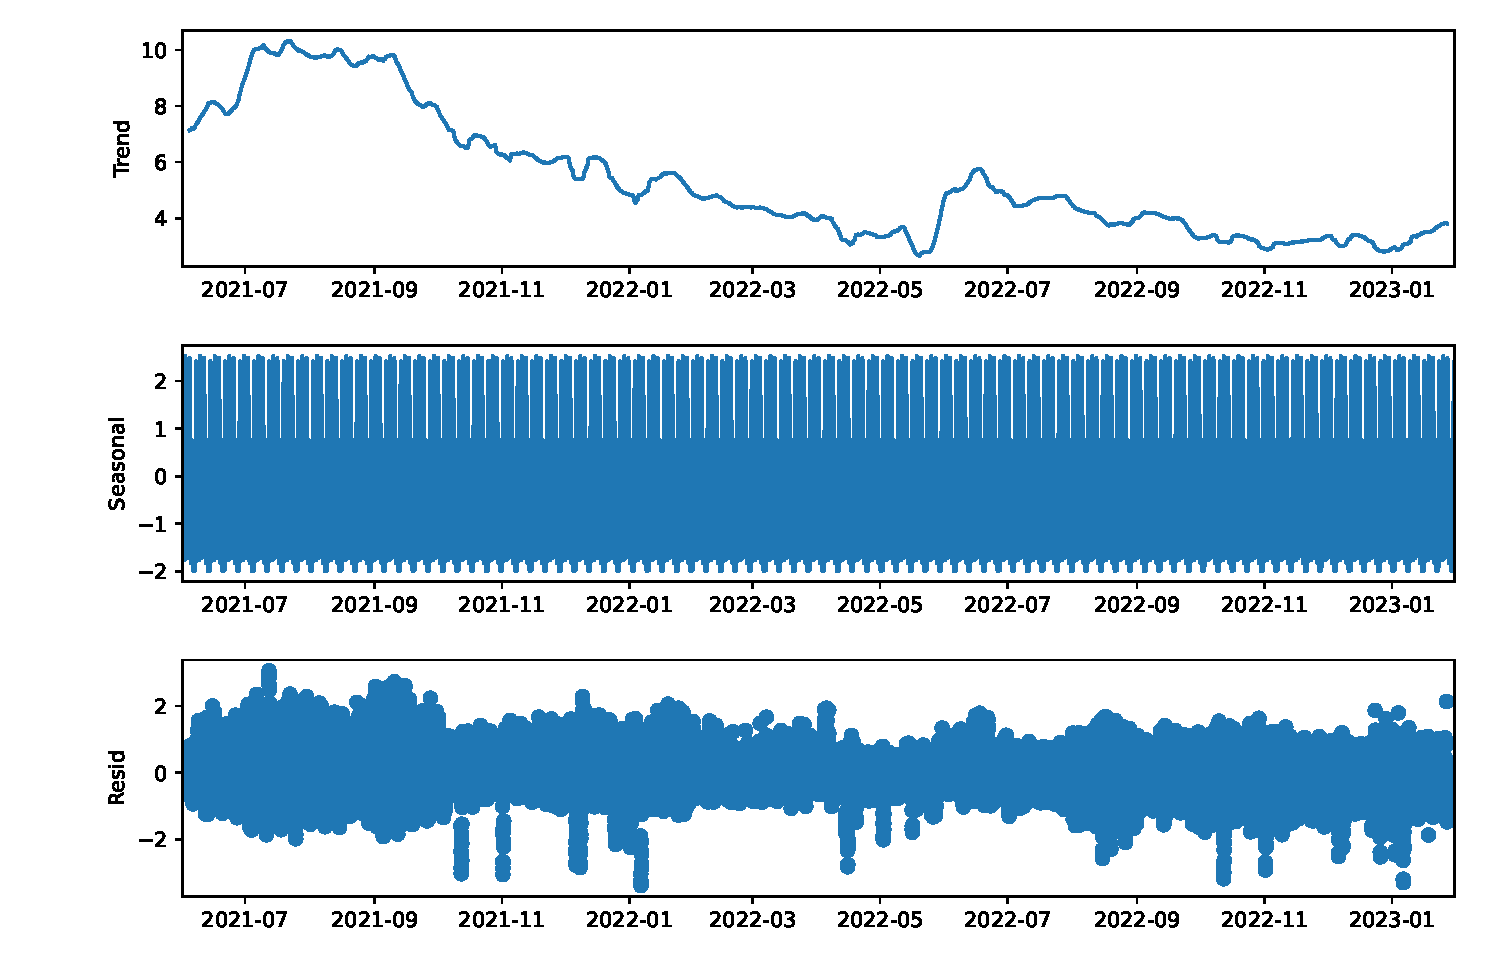
\includegraphics[width=0.5\textwidth]{images/demand/hourly_decomposition_week_period}
\caption{The time series decomposition of the hourly aggregated consumption over the customers considering as period of the time series a week.}
\label{fig:demanddecomposition}
\end{figure}

The auto-correlation of the hourly aggregated consumption over the customers is reported in figure~\ref{fig:demandcorrelation}.
It shows a high auto-correlation value in the close time lags and also at every 24 hours, along with an even higher value at a one-week distance.
This indicates that the consumption data from the closest time lags, particularly up to three closest ones, as well as those corresponding to the same hour in the preceding days and even better in the preceding weeks, may be valuable features for predicting a time instant's demand.
A reasonable balance can be achieved by incorporating the consumption data from the past 14 days.

\begin{figure}[H]
\centering
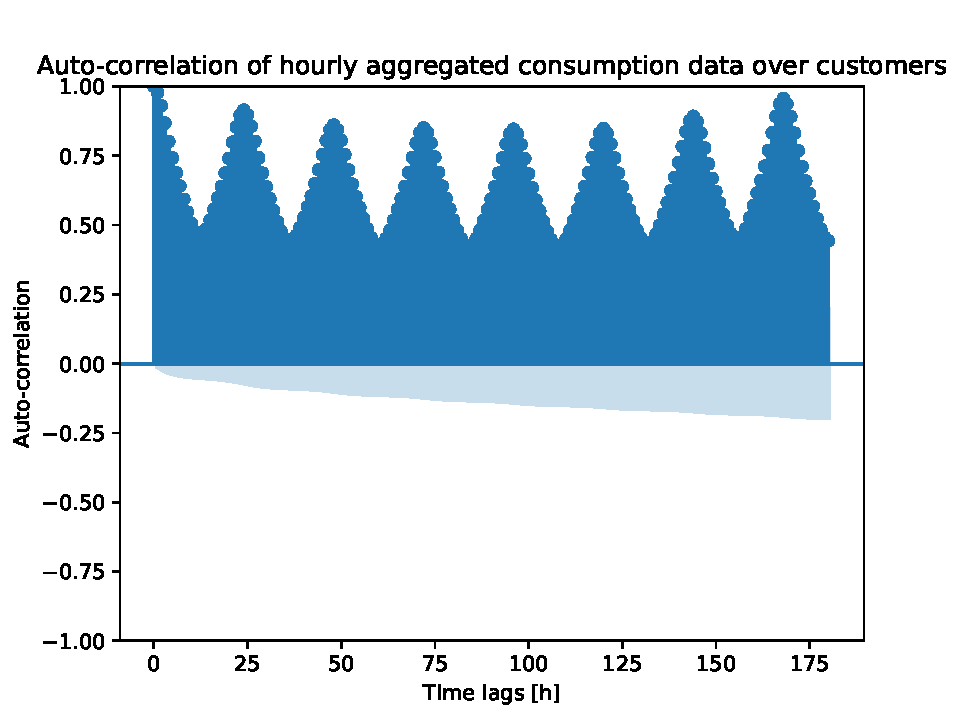
\includegraphics[width=0.4\textwidth]{images/demand/hourly_correlation_week_range}
\caption{The auto-correlation of the hourly aggregated consumption over the customers.}
\label{fig:demandcorrelation}
\end{figure}

The coefficients given by the Fourier transform for the hourly aggregated consumption over the customers are reported in figure~\ref{fig:demandft}.
The graphical representation shows 2 main frequencies, one representing the weekly periodicity and one the daily periodicity.
Other minor peaks are present mostly at multiples of the 1/week frequency.

\begin{figure}[H]
\centering
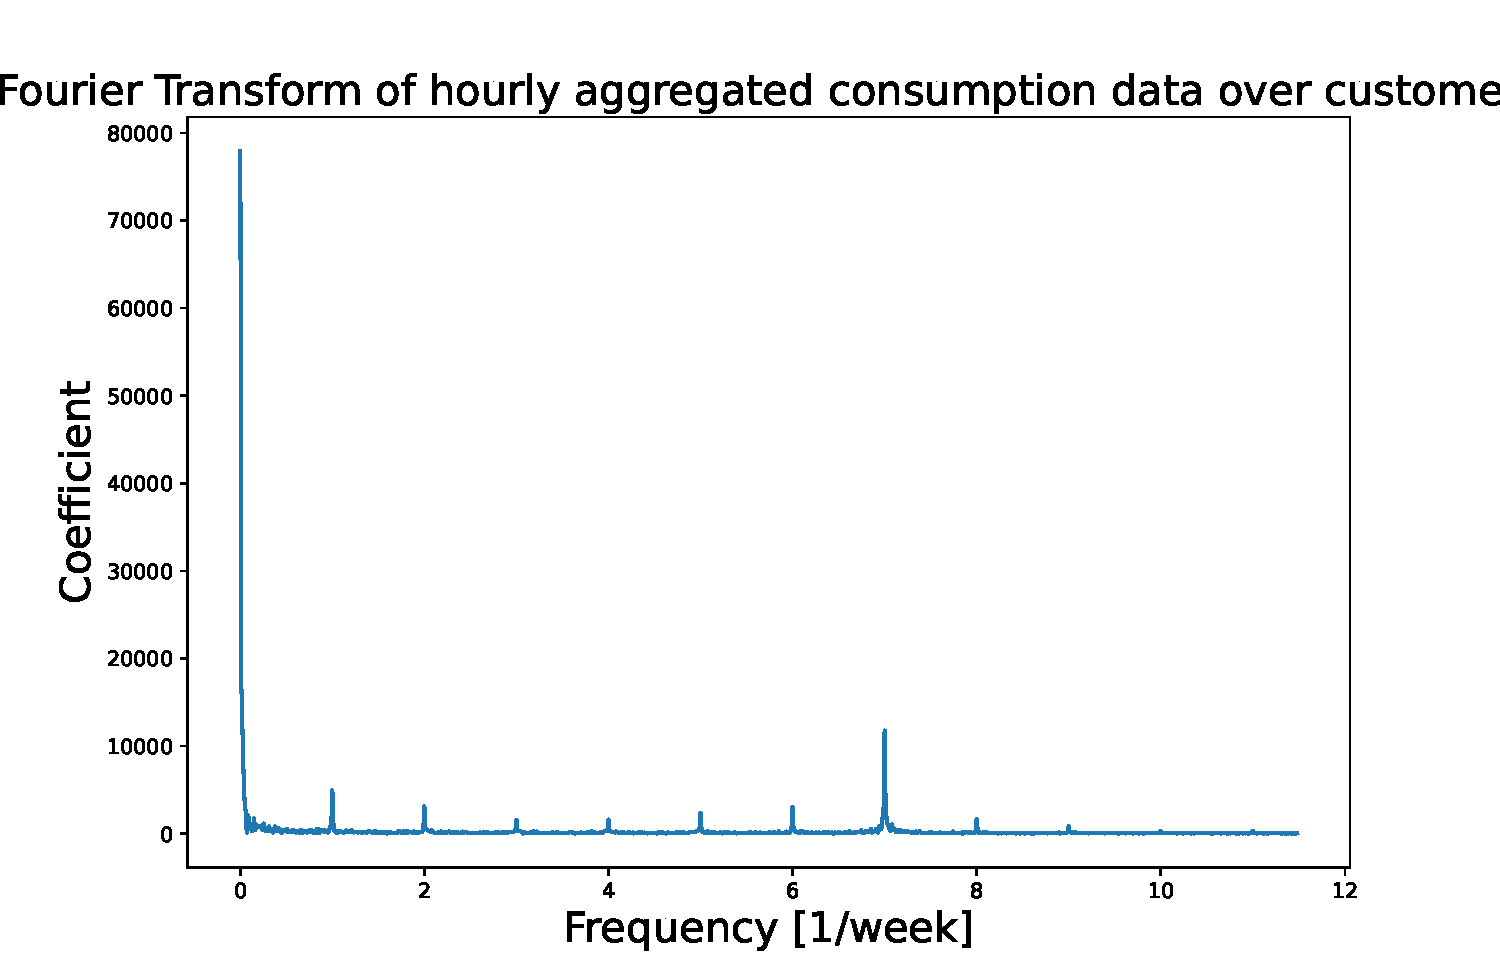
\includegraphics[width=0.4\textwidth]{images/demand/ft_hour_week}
\caption{The coefficients given by the Fourier transform for the hourly aggregated consumption over the customers.}
\label{fig:demandft}
\end{figure}

The daily aggregated consumption over the customers is reported in figure~\ref{fig:demanddataplotday}.
Aggregating the data on a daily basis, it is possible to more clearly observe the weekly pattern of consumption, which exhibits an increase on weekdays and a decrease on weekends.

\begin{figure}[H]
\centering
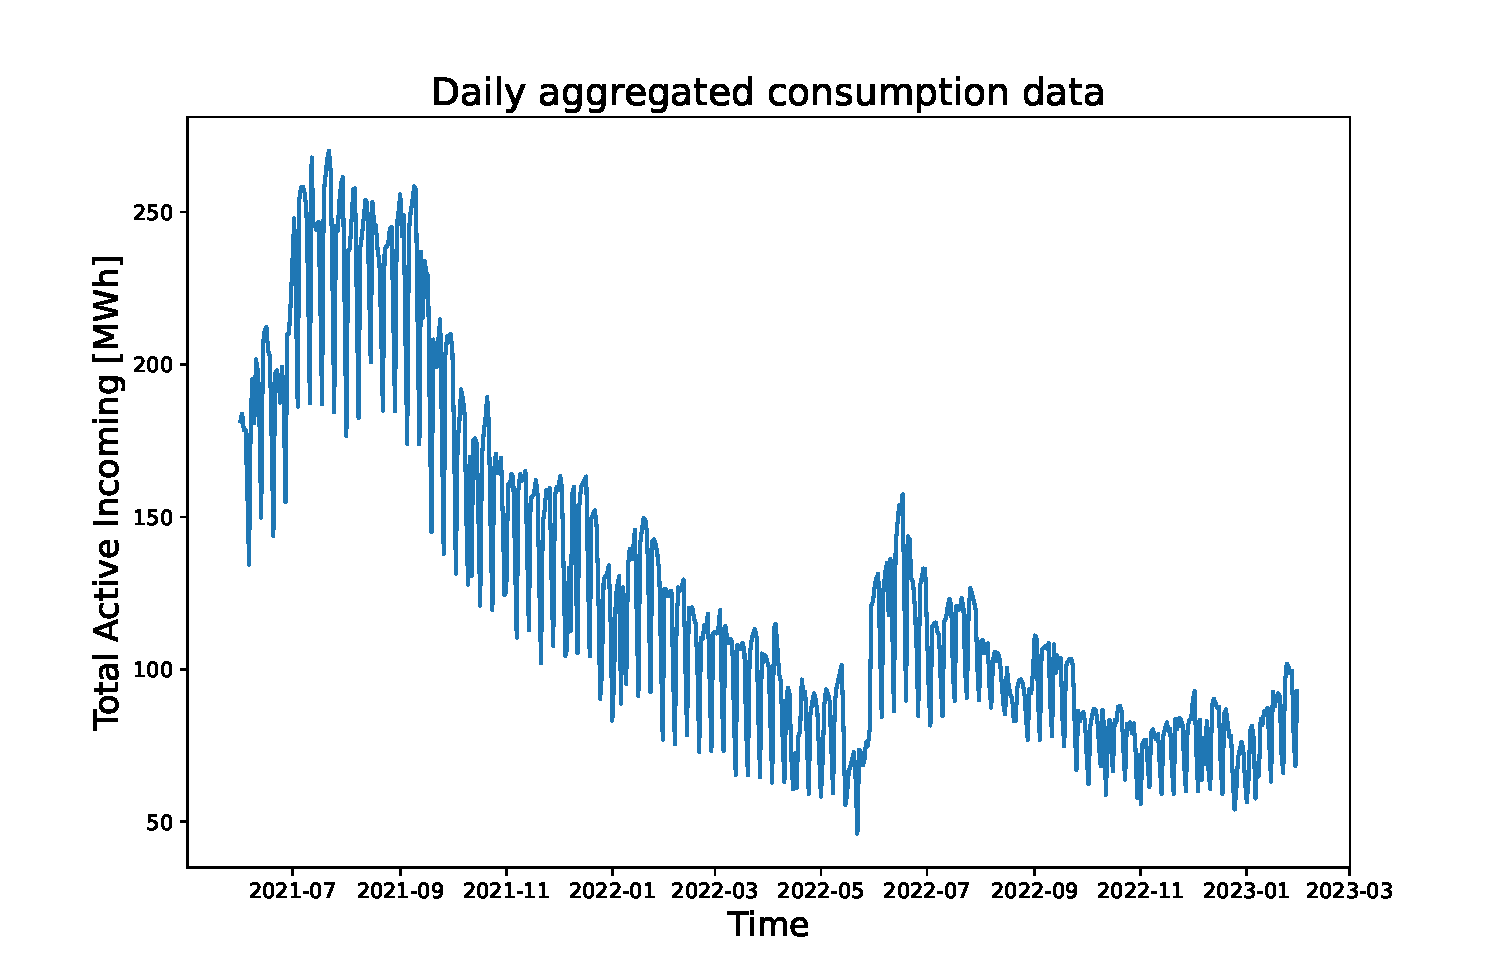
\includegraphics[width=0.5\textwidth]{images/demand/data_day_aggregated_plot}
\caption{The daily aggregated consumption over the customers.}
\label{fig:demanddataplotday}
\end{figure}

Figure~\ref{fig:demanddecompositionday} shows the time series decomposition of the daily aggregated consumption over the customers, using an additive model with a period of one week.
The decomposition is consistent with the hourly aggregated consumption over the customers.

\begin{figure}[H]
\centering
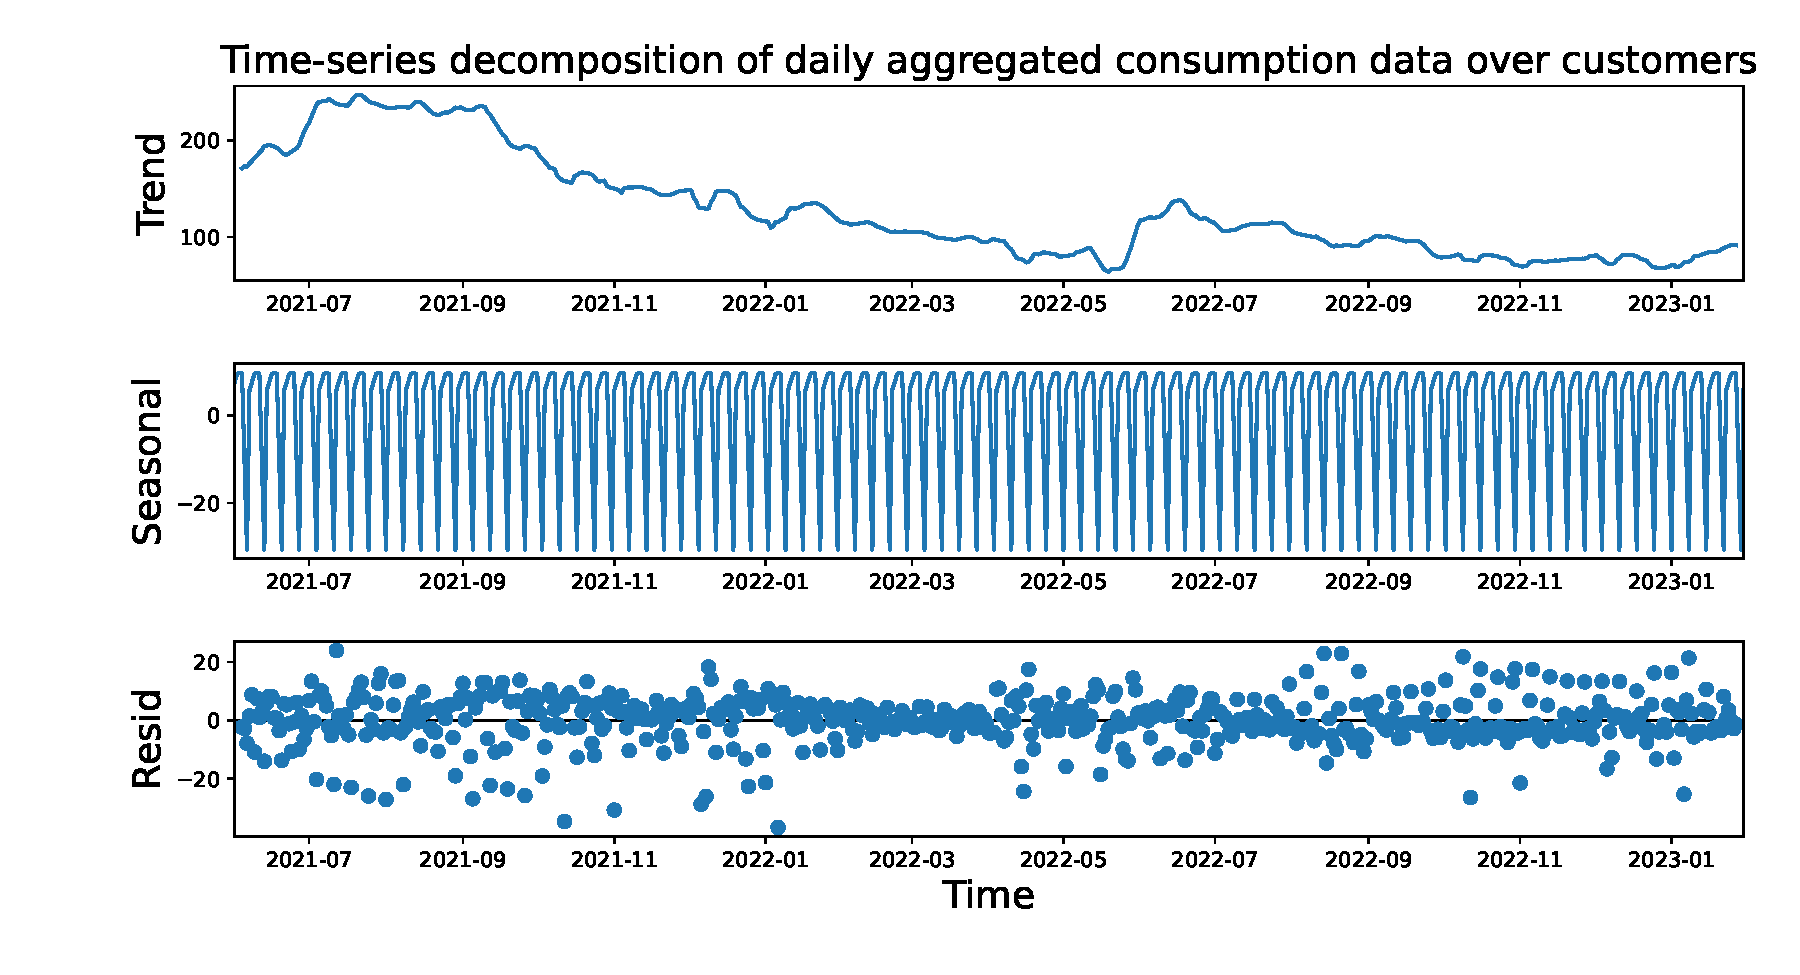
\includegraphics[width=0.5\textwidth]{images/demand/daily_aggregated_decomposition}
\caption{The time series decomposition of the daily aggregated consumption over the customers considering as period of the time series a week.}
\label{fig:demanddecompositionday}
\end{figure}

The auto-correlation of the daily aggregated consumption over the customers is reported in figure~\ref{fig:demandcorrelationday}.
It shows a high auto-correlation value in the closest time lag, with an even greater value at every week lag.
This suggests that useful features, since highly correlated, for predicting a time instant's demand may be the closest ones, but also those from the same day of the week in the previous weeks.
A good trade-off can be achieved by considering the consumption data in the previous 14 days.

\begin{figure}[H]
\centering
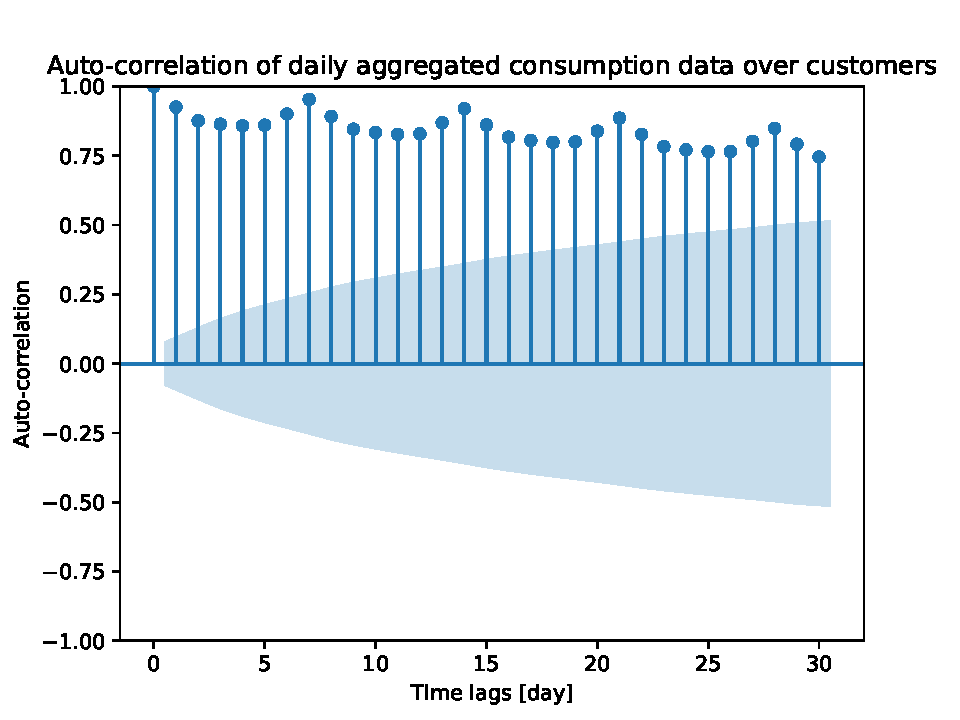
\includegraphics[width=0.4\textwidth]{images/demand/daily_aggregated_correlation}
\caption{The auto-correlation of the daily aggregated consumption over the customers.}
\label{fig:demandcorrelationday}
\end{figure}

The coefficients given by the Fourier transform for the daily aggregated consumption over the customers are reported in figure~\ref{fig:demandftday}.
The graphical representation shows 1 main frequency representing the weekly periodicity and other minor peaks at multiples of the 1/week frequency.

\begin{figure}[H]
\centering
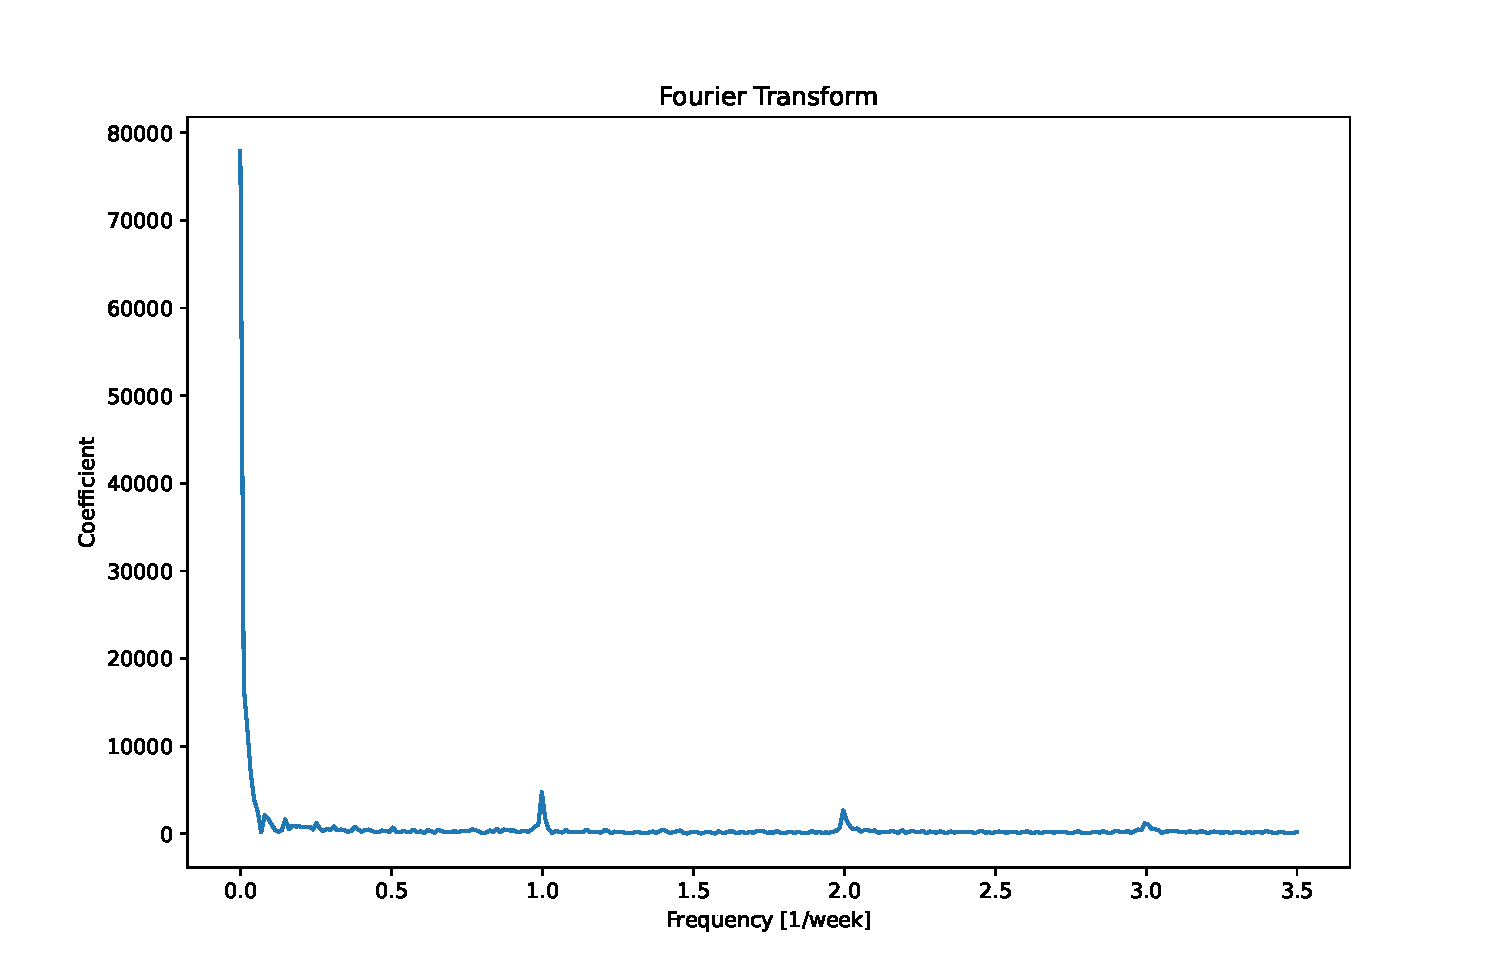
\includegraphics[width=0.4\textwidth]{images/demand/ft_day}
\caption{The coefficients given by the Fourier transform for the daily aggregated consumption over the customers.}
\label{fig:demandftday}
\end{figure}

Basic data is enhanced with the air temperature, the apparent temperature, and the relative humidity since they are considered the only weather features capable of influencing customers' energy consumption.
To assess the relationship between these weather variables and the aggregated consumption over the customers, two correlation coefficients were used: Pearson's correlation coefficient and Spearman's rank correlation coefficient.
Pearson's correlation coefficient measures the strength of the linear relationship between two variables, while Spearman's rank correlation coefficient measures the strength of the monotonic relationship.
The pearsonr and spearmanr methods of the SciPy library\footnote{ \url{https://scipy.org/} } were used to compute the correlation with weather data.
The results showed that the hourly aggregated consumption over the customers had:
\begin{itemize}
  \item a Pearson correlation coefficient of 0.4480 and a Spearman's rank correlation coefficient of 0.4378 with respect to the air temperature;
  \item a Pearson correlation coefficient of 0.4475 and a Spearman's rank correlation coefficient of 0.4368 with respect to the apparent temperature;
  \item a Pearson correlation coefficient of -0.2689 and a Spearman's rank correlation coefficient of -0.3173 with respect to the relative humidity.
\end{itemize}
It can be noticed that both the coefficients indicate a moderate correlation between the weather variables and consumption, this suggests that incorporating weather data into the prediction models could be useful.

The results showed that the daily aggregated consumption over the customers had:
\begin{itemize}
  \item a Pearson correlation coefficient of 0.3898 and a Spearman's rank correlation coefficient of 0.3119 with respect to the air temperature;
  \item a Pearson correlation coefficient of 0.3823 and a Spearman's rank correlation coefficient of 0.3114 with respect to the apparent temperature;
  \item a Pearson correlation coefficient of -0.0908 and a Spearman's rank correlation coefficient of -0.1547 with respect to the relative humidity.
\end{itemize}
It can be noticed that both the coefficients decreased considering the daily data meaning that the mean weather data over the day is less correlated to the daily aggregated consumption over the customers, compared to the hourly granularity.

After this data analysis, the specific parameters used in the models can be explained more in detail.
The parameters for the different models were tested and verified on training data to result in the best-performing models, this was done by trying different values and configurations.
The baseline approaches are built considering the repetition of past days and weeks since data presents a high correlation with that time instants and could lead to a reasonable baseline performance to achieve.
The SARIMA model considers the week as the period for seasonal differencing since data presents a high correlation with that time instants and the model can try to take advantage of the weekly seasonality.
The support vector regressor model uses a radial basis function kernel with a configuration of the C parameter (regularization parameter of squared l2 penalty) to 1.0 to penalize the complexity of the model, and the epsilon parameter defining the epsilon-tube for no penalty to 0.1 as a trade-off between accuracy and generalization.
The hist gradient boosting regressor model uses as loss the absolute error since this was the supported metric closer to our evaluation metric.
The learning rate was set to 0.1, 100 estimators were used and l2 regularization was not set.
The parameters for tree definition are 31 as the maximum number of leaves, depth is not constrained, 20 as the minimum number of samples per leaf, and 255 as the maximum number of bins.
For the extreme gradient boosting regressor model, tree-based models were used and the construction algorithm is automatically chosen by heuristic to choose the fastest method.
It uses a squared loss since this was the supported metric closer to our evaluation metric.
The learning rate was set to 0.3, 100 estimators were used and l2 regularization was set with a weight of 1.0.
The parameters for tree definition are 6 as the maximum depth, and the maximum number of leaves is not constrained.
The Prophet model was built keeping the default parameters for automatically detecting seasonalities and best fitting the training data.

The LSTM model was designed as a 2-layer model with 24 Bidirectional LSTM units in the first layer which use rectified linear unit (ReLU) activation function and sigmoid as recurrent activation function with both dropout and recurrent dropout of 0.02.
Batch normalization is then applied before entering the second layer composed of 16 Bidirectional LSTM units which use ReLU activation function and sigmoid as recurrent activation function without dropout and recurrent dropout.
The output of the layer goes inside a dense unit to output the final prediction.
The model is trained using mean absolute percentage error as loss and Nadam (a version of Adam integrating the concept of Nesterov momentum) as optimizer with a learning rate of 0.005.

The GRU model was designed as a 3-layer model with 24 Bidirectional GRU units in the first layer which use ReLU activation function and sigmoid as recurrent activation function with both dropout and recurrent dropout of 0.02.
Subsequently, the second layer is composed of 16 Bidirectional GRU units which use ReLU activation function and sigmoid as recurrent activation function without dropout and recurrent dropout.
The output of the second layer goes inside a third dense layer composed of 4 units with ReLU activation function before entering the final dense unit to output the final prediction.
The model is trained using mean absolute percentage error as loss and Nadam as optimizer with a learning rate of 0.005.

The CNN model was designed as a 3-layer model with a first layer composed of 24 1D Convolutional units with a kernel size of 5 which uses ReLU activation function.
A 1D max polling operation is applied before entering the second layer composed of 16 1D Convolutional units with a kernel size of 3 which use ReLU activation function.
A 1D max polling operation is applied before the flattening operation and entering the third dense layer composed of 4 units with ReLU activation function.
The output of the layer goes inside a dense unit to output the final prediction.
The model is trained using mean absolute percentage error as loss and Nadam as optimizer with a learning rate of 0.005.

The TFT model was configured with 2 LSTM layers with 16 as hidden size, 4 as attention size, and 8 as hidden continuous size.
The dropout is set to 0.02.
The model is trained using mean absolute percentage error as loss and Nadam as optimizer with a learning rate of 0.005.

12 splits were used for block validation with a test size of a month each time, namely 30 days of data.
For the hourly granularity, the models start with 5977 entries as training and predict every time 720 entries until reaching the last prediction instant where the model has a training size of 13897.
The results for hourly granularity are reported in table~\ref{tab:demandhourlyresults}.
Entries are sorted by best MAPE using the last split as the test set.
The blocked k-fold cross-validation suggests that the one-week baseline has the best MAPE, but looking at the last split this is not confirmed.
This is probably due to the fact that overall the weekly repetition seems to be quite effective over the year, but there are better approaches that with the increase of training data perform better, this can be the case in GRU and CNN since the results on the last split are quite good compared to the mean MAPE obtained over the splits.
This can be explained by the fact that, due to their complexity, these models require more data and in the first splits there was not even a single year of data, so they didn't even have the possibility to infer a possible annual seasonality.
Results seem also to confirm that not always sophisticated models perform better and some of them are no better than a baseline.
Models treated in the literature that are performing well in similar tasks can also not be suited for this specific use case.
Data makes a big difference and with a low amount of data, it is difficult for some complex networks to perform well and generalize.
Instead, the TFT approach seems to have pretty much the same MAPE over the considered splits confirming the power of this architecture despite the limited data
In contrast, the boosters that have a good blocked k-fold MAPE on the last split do not perform well.

\begin{table}[H]
\centering
\begin{tabular}{|c|c|c|}
\hline
\textbf{Model} & \textbf{Blocked k-fold} & \textbf{Test on the last split}\\
 & \textbf{cross-validation MAPE} & \textbf{MAPE}\\
\hline
TFT & 15.00 $\pm$ 4.31 & 14.76\\
\hline
GRU & 30.77 $\pm$ 14.48 & 16.82\\
\hline
CNN & 34.64 $\pm$ 15.76 & 17.49\\
\hline
One Week Baseline & 12.94 $\pm$ 4.27 & 17.55\\
\hline
SARIMA & 15.44 $\pm$ 4.57 & 18.47\\
\hline
One Day Baseline & 22.86 $\pm$ 7.07 & 20.54\\
\hline
LSTM & 34.08 $\pm$ 11.92 & 23.18\\
\hline
HistGradientBoostingRegressor & 14.54 $\pm$ 5.51 & 29.33\\
\hline
SVR & 61.80 $\pm$ 22.63 & 29.47\\
\hline
Prophet & 28.68 $\pm$ 7.07 & 31.62\\
\hline
XGBRegressor & 16.88 $\pm$ 8.08 & 37.81\\
\hline
\end{tabular}
\caption{Table summarizing the results for hourly granularity.}
\label{tab:demandhourlyresults}
\end{table}

The results for hourly granularity at forecasting time on the last time slot including also the combinations of different techniques and the AutoML approach are reported in table~\ref{tab:demandhourlyresultsforecast}.
The combination of the previous techniques was performed by combining one-day baseline, one-week baseline, and Prophet with possibly one of LSTM, GRU, or CNN with the intent of trying to improve the robustness of DL models with some stable baselines and Prophet model which internally automatically deals with seasonalities, even though for this task it is not performing very well.
The AutoML approach uses the mean MAPE forecasting as loss and it is launched for 10 hours with a maximum function evaluation time of 2 hours.
Then the best ensemble of the found models is returned and can be used to forecast.
In the table, it is also reported the performance on the one-week horizon, namely 7 days of data, from which it is possible to gain more insights on the models' forecasts.
Including also combinations and AutoML, there are a few observations that can be done.
The combinations of DL models and the one-week baseline are the most beneficial, reducing by many points the MAPE of the techniques on the one-month time horizon.
This suggests that it can make sense to investigate the concept of ensemble learning further and optimize this combination at training time to possibly have stronger results at forecasting time.
AutoML has great potential and obtains very good results compared to many other models.
Potentially providing more total training time it can be further optimized to reach better performance.
TFT still dominates on the one-month MAPE but not on the one-week one on which the one-week baseline and many combinations but also SARIMA and hist gradient boosting regressor perform better.
This confirmed that the strength of TFT is to have good performance and preserve it also on larger prediction horizons.

\begin{table}[H]
\centering
\begin{tabular}{|c|c|c|}
\hline
\textbf{Model} & \textbf{Forecast on the last split} & \textbf{Forecast on the last split}\\
 & \textbf{one-week MAPE} & \textbf{one-month MAPE}\\
\hline
TFT & 13.71 & 14.76\\
\hline
GRU + One Week Baseline & 11.79 & 14.79\\
\hline
CNN + One Week Baseline & 11.84 & 15.39\\
\hline
GRU & 17.25 & 16.82\\
\hline
AutoML & 14.68 & 16.96\\
\hline
CNN + One Week Baseline + & 15.43 & 17.13\\
Prophet & & \\
\hline
CNN + One Day Baseline + & 13.60 & 17.25\\
One Week Baseline + Prophet & & \\
\hline
GRU + One Day Baseline + & 13.25 & 17.33\\
One Week Baseline + Prophet & & \\
\hline
GRU + One Week Baseline + & 15.63 & 17.37\\
Prophet & & \\
\hline
CNN & 14.59 & 17.49\\
\hline
One Week Baseline & 10.87 & 17.55\\
\hline
LSTM + One Week Baseline + & 13.16 & 17.89\\
Prophet & & \\
\hline
LSTM + One Day Baseline + & 12.58 & 18.10\\
One Week Baseline + Prophet & & \\
\hline
LSTM + One Week Baseline & 14.42 & 18.11\\
\hline
SARIMA & 12.28 & 18.47\\
\hline
One Day Baseline & 14.78 & 20.54\\
\hline
One Day Baseline + & 15.15 & 20.97\\
One Week Baseline + Prophet & & \\
\hline
One Week Baseline + Prophet & 19.02 & 22.80\\
\hline
LSTM & 20.94 & 23.18\\
\hline
HistGradientBoostingRegressor & 13.00 & 29.33\\
\hline
SVR & 29.06 & 29.47\\
\hline
Prophet & 33.94 & 31.62\\
\hline
XGBRegressor & 17.84 & 37.81\\
\hline
\end{tabular}
\caption{Table summarizing the results for hourly granularity at forecasting time.}
\label{tab:demandhourlyresultsforecast}
\end{table}

The forecasts produced by the TFT model for the last split in comparison to the actual values are reported in figure~\ref{fig:demandtfthourlyforecasts}.
It can be noticed that for the first week, it follows the signal very accurately, the second and third weeks are pretty good but it is missing the peaks over the day and the last week is decreasing while the actual values have high peaks.
The absolute percentage error of forecasts produced by the TFT model for the last split in comparison to the actual values is reported in figure~\ref{fig:demandtfthourlyforecastsmape}.
It can be shown that except for some peaks, the percentage error stays below 30\%, with most values around 10\%.
Finally, the scatter plot representing the error of the forecasts produced by the TFT model for the last split in comparison to the actual values is reported in figure~\ref{fig:demandtfthourlyforecastsscatterplot}.
This scatter plot demonstrates that there is no bias and can be also noticed that when the predicted values are low also the error is limited, while when the prediction is high there are both high positive and negative errors.

\begin{figure}[H]
\centering
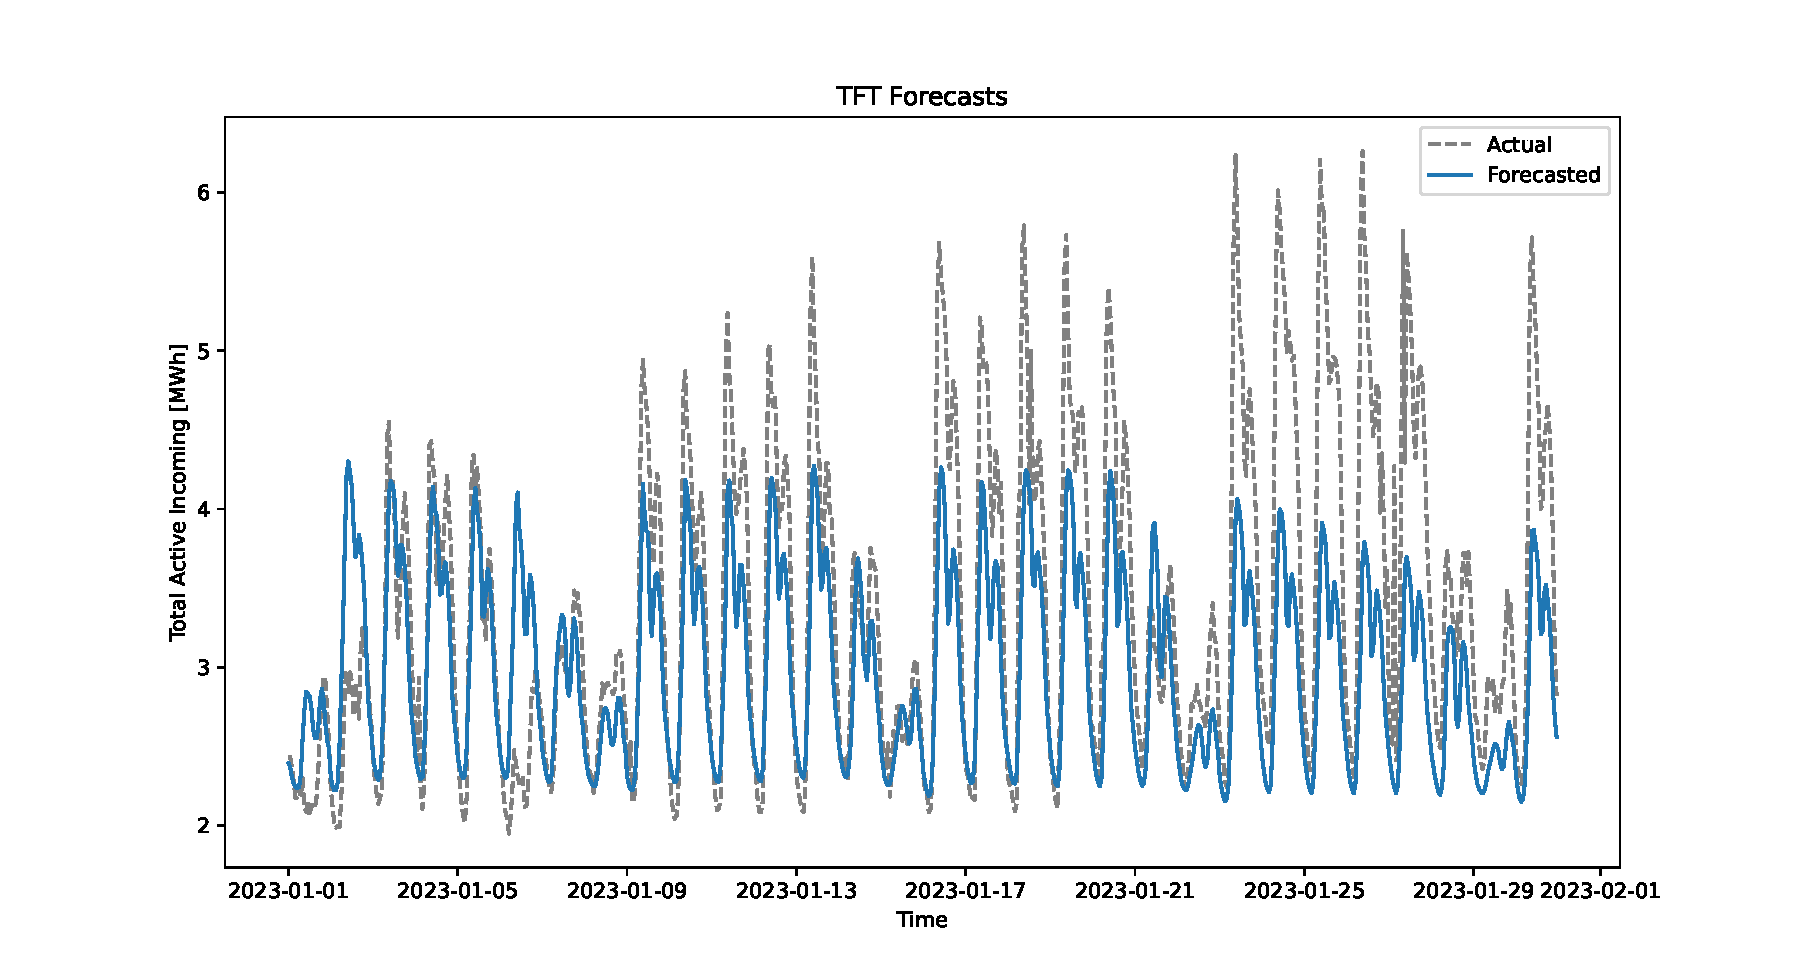
\includegraphics[width=1\textwidth]{images/demand/TFT}
\caption{The forecasts produced by the temporal fusion transoformer model for the last split in comparison to the actual values.}
\label{fig:demandtfthourlyforecasts}
\end{figure}

\begin{figure}[H]
\centering
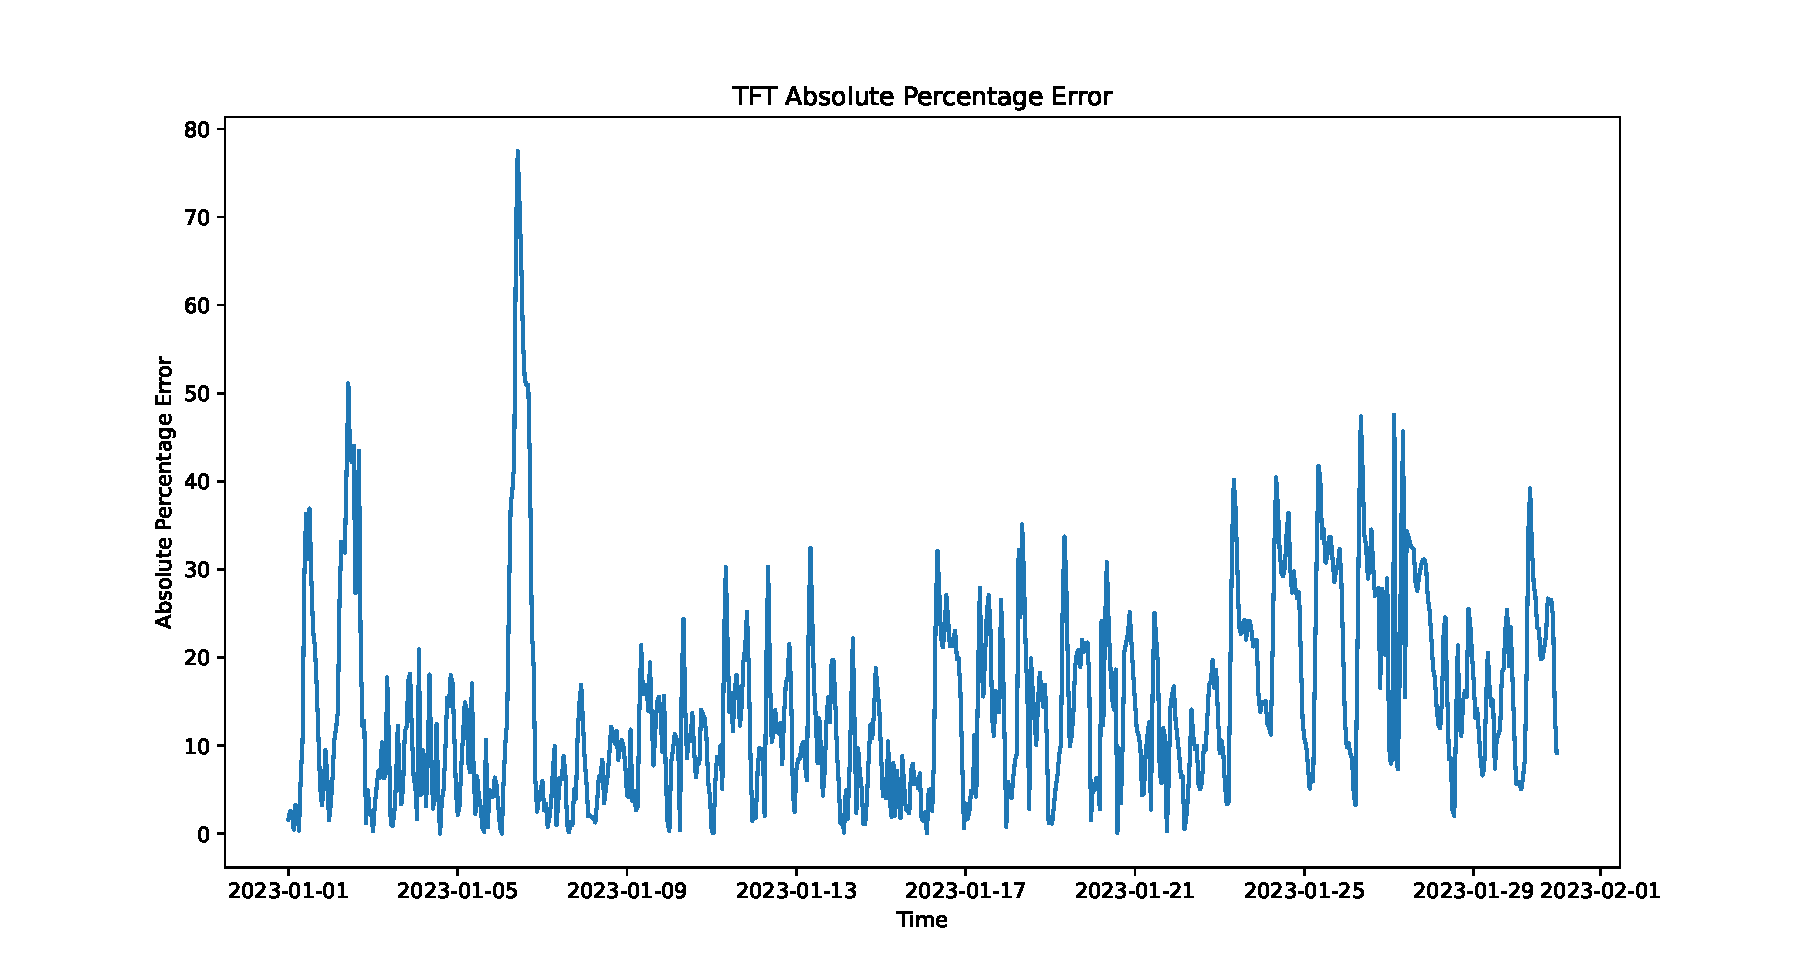
\includegraphics[width=1\textwidth]{images/demand/TFT_mape}
\caption{The absolute percentage error of forecasts produced by the temporal fusion transoformer model for the last split in comparison to the actual values.}
\label{fig:demandtfthourlyforecastsmape}
\end{figure}

\begin{figure}[H]
\centering
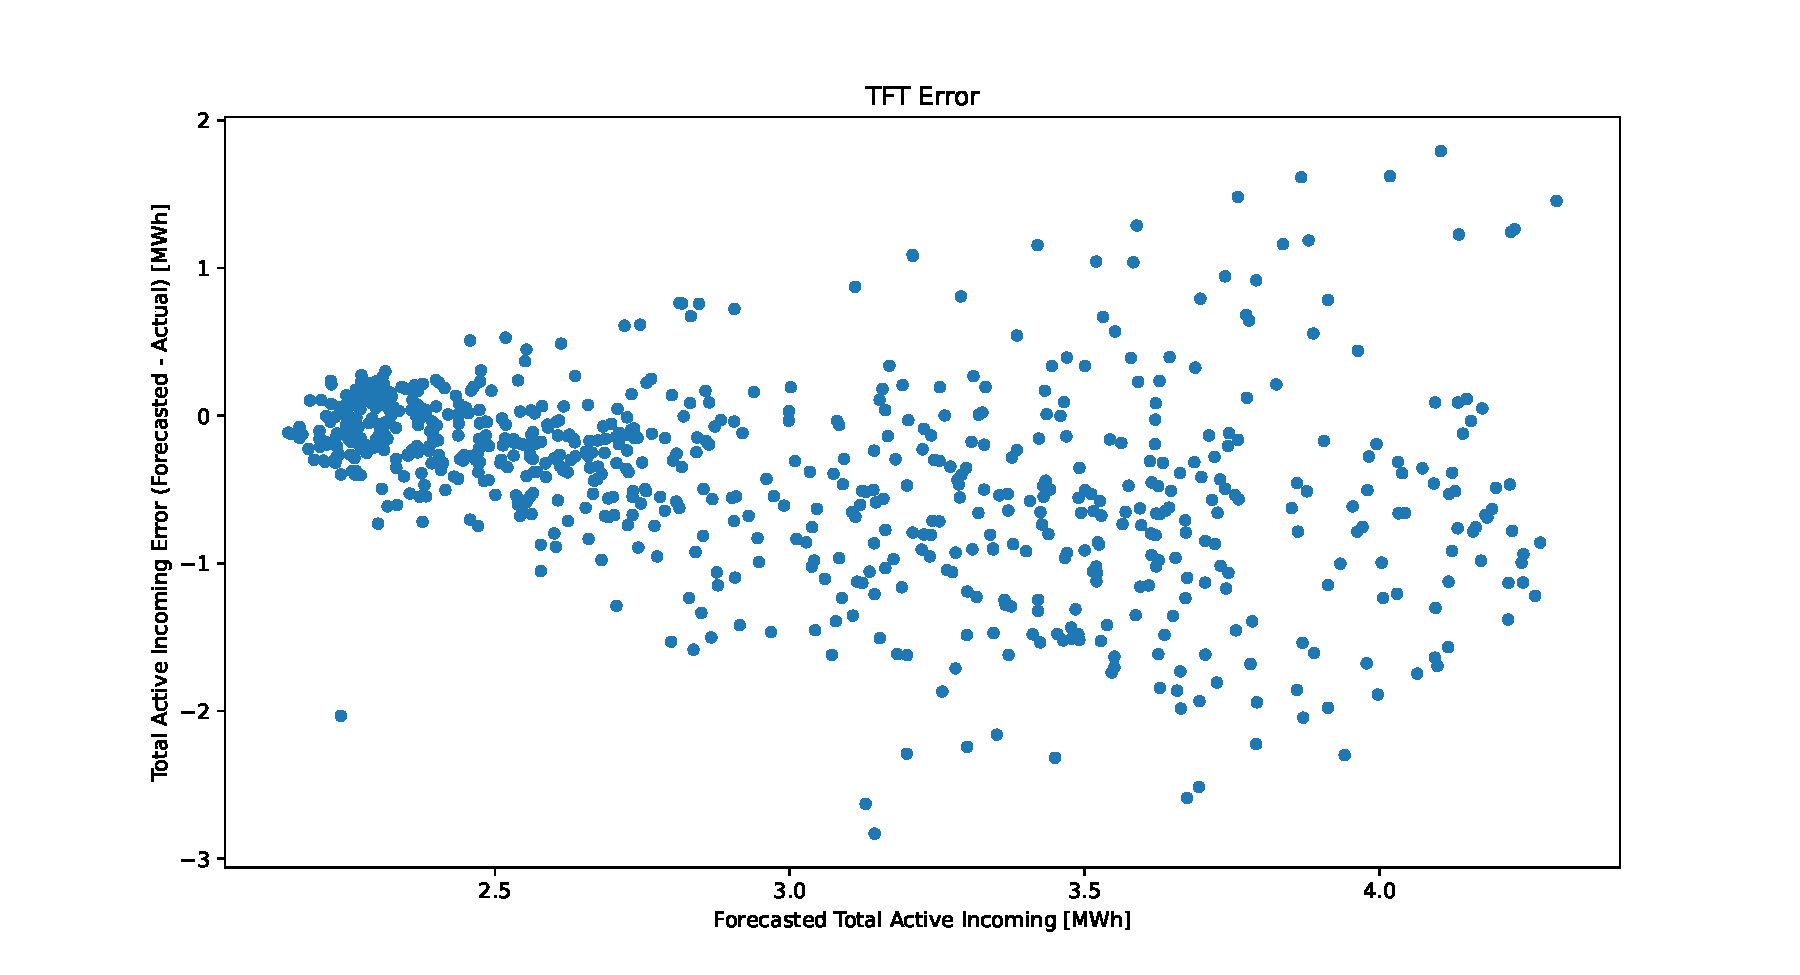
\includegraphics[width=1\textwidth]{images/demand/TFT_error_scatter_plot_predicted}
\caption{The scatter plot representing the error of the forecasts produced by the temporal fusion transoformer model for the last split in comparison to the actual values.}
\label{fig:demandtfthourlyforecastsscatterplot}
\end{figure}

For the daily granularity, the models start with 249 entries as training and predict every time 30 entries until reaching the last prediction instant where the model has a training size of 579.
The results for daily granularity are reported in table~\ref{tab:demanddailyresults}.
In this case, TFT is no longer the best-performing model, probably due to the fact of 24 times less quantity of data due to the daily granularity.
Though, it is still a well-performing model on both blocked k-fold cross-validation and last split results.
LSTM and CNN perform better in terms of the last split MAPE but present a high blocked k-fold MAPE, as in the case of the hourly granularity probably that to the increase of data, the results on the last time slots improved in a significant way.
Also, the boosters present very good results on the last time split and also on the blocked k-fold validation showing consistency over time and good results also with few training data. 

\begin{table}[H]
\centering
\begin{tabular}{|c|c|c|}
\hline
\textbf{Model} & \textbf{Blocked k-fold} & \textbf{Test on the last split}\\
 & \textbf{cross-validation MAPE} & \textbf{MAPE}\\
\hline
CNN & 50.55 $\pm$ 36.81 & 7.49\\
\hline
XGBRegressor & 12.96 $\pm$ 4.36 & 7.65\\
\hline
HistGradientBoostingRegressor & 13.02 $\pm$ 5.54 & 9.81\\
\hline
LSTM & 29.60 $\pm$ 13.81 & 14.51\\
\hline
TFT & 13.73 $\pm$ 5.06 & 14.88\\
\hline
One Week Baseline & 11.50 $\pm$ 4.78 & 18.40\\
\hline
SARIMA & 11.92 $\pm$ 7.04 & 19.63\\
\hline
GRU & 28.76 $\pm$ 29.26 & 20.47\\
\hline
One Day Baseline & 22.80 $\pm$ 8.21 & 21.51\\
\hline
Prophet & 19.06 $\pm$ 10.81 & 26.33\\
\hline
SVR & 53.63 $\pm$ 22.39 & 39.82\\
\hline
\end{tabular}
\caption{Table summarizing the results for daily granularity.}
\label{tab:demanddailyresults}
\end{table}

The results for daily granularity at forecasting time on the last time slot including also the combinations of different techniques and the AutoML approach are reported in table~\ref{tab:demanddailyresultsforecast}.
In this case, the impact of the combinations is not so evident and does not improve the results in all the cases.
AutoML presents not very good results being worse than the one-week baseline, this is probably due to the scarcity of training data and the fact of AutoML of trying very complex architectures when also simple ones may work well in certain cases.
It can also be noticed that surprisingly for some of the best-performing models the MAPE on the first week of data is higher than the one on the whole month of data.
This probably can be explained by the fact that the first week of the last split has a less regular pattern due to the Christmas holidays compared to the following ones.

\begin{table}[H]
\centering
\begin{tabular}{|c|c|c|}
\hline
\textbf{Model} & \textbf{Forecast on the last split} & \textbf{Forecast on the last split}\\
 & \textbf{one-week MAPE} & \textbf{one-month MAPE}\\
\hline
CNN & 8.36 & 7.49\\
\hline
XGBRegressor & 11.78 & 7.65\\
\hline
HistGradientBoostingRegressor & 12.42 & 9.81\\
\hline
CNN + One Week Baseline & 8.33 & 12.28\\
\hline
LSTM + One Week Baseline & 11.19 & 12.91\\
\hline
LSTM & 18.21 & 14.51\\
\hline
TFT & 12.65 & 14.88\\
\hline
LSTM + One Week Baseline + & 8.81 & 15.91\\
Prophet & & \\
\hline
CNN + One Week Baseline + & 11.34 & 16.96\\
Prophet & & \\
\hline
LSTM + One Day Baseline + & 9.82 & 17.29\\
One Week Baseline + Prophet & & \\
\hline
CNN + One Day Baseline + & 10.88 & 17.88\\
One Week Baseline + Prophet & & \\
\hline
One Week Baseline & 9.63 & 18.40\\
\hline
GRU + One Week Baseline & 9.15 & 19.18\\
\hline
SARIMA & 11.23 & 19.63\\
\hline
GRU & 10.87 & 20.47\\
\hline
AutoML & 10.61 & 20.98\\
\hline
GRU + One Day Baseline + & 11.29 & 21.34\\
One Week Baseline + Prophet & & \\
\hline
One Day Baseline & 13.14 & 21.51\\
\hline
GRU + One Week Baseline + & 11.89 & 21.56\\
Prophet & & \\
\hline
One Day Baseline + & 11.72 & 21.69\\
One Week Baseline + Prophet & & \\
\hline
One Week Baseline + Prophet & 12.83 & 22.21\\
\hline
Prophet & 17.35 & 26.33\\
\hline
SVR & 58.09 & 39.82\\
\hline
\end{tabular}
\caption{Table summarizing the results for hourly granularity at forecasting time.}
\label{tab:demanddailyresultsforecast}
\end{table}

The forecasts produced by the CNN model for the last split in comparison to the actual values are reported in figure~\ref{fig:demandcnndailyforecasts}.
It can be noticed that for the first three weeks, it follows the signal very accurately and the last week is increasing correctly but not enough as the actual values.
The absolute percentage error of forecasts produced by the CNN model for the last split in comparison to the actual values is reported in figure~\ref{fig:demandcnndailyforecastsmape}.
It can be shown that except for some peaks, the percentage error stays below 10\%.
Finally, the scatter plot representing the error of the forecasts produced by the CNN model for the last split in comparison to the actual values is reported in figure~\ref{fig:demandcnndailyforecastsscatterplot}.
This scatter plot demonstrates that there is no bias even though it seems that when predicting high values it is missing some extra quantity in the forecasts, this is probably true in the specific considered last split and in particular the last week.

\begin{figure}[H]
\centering
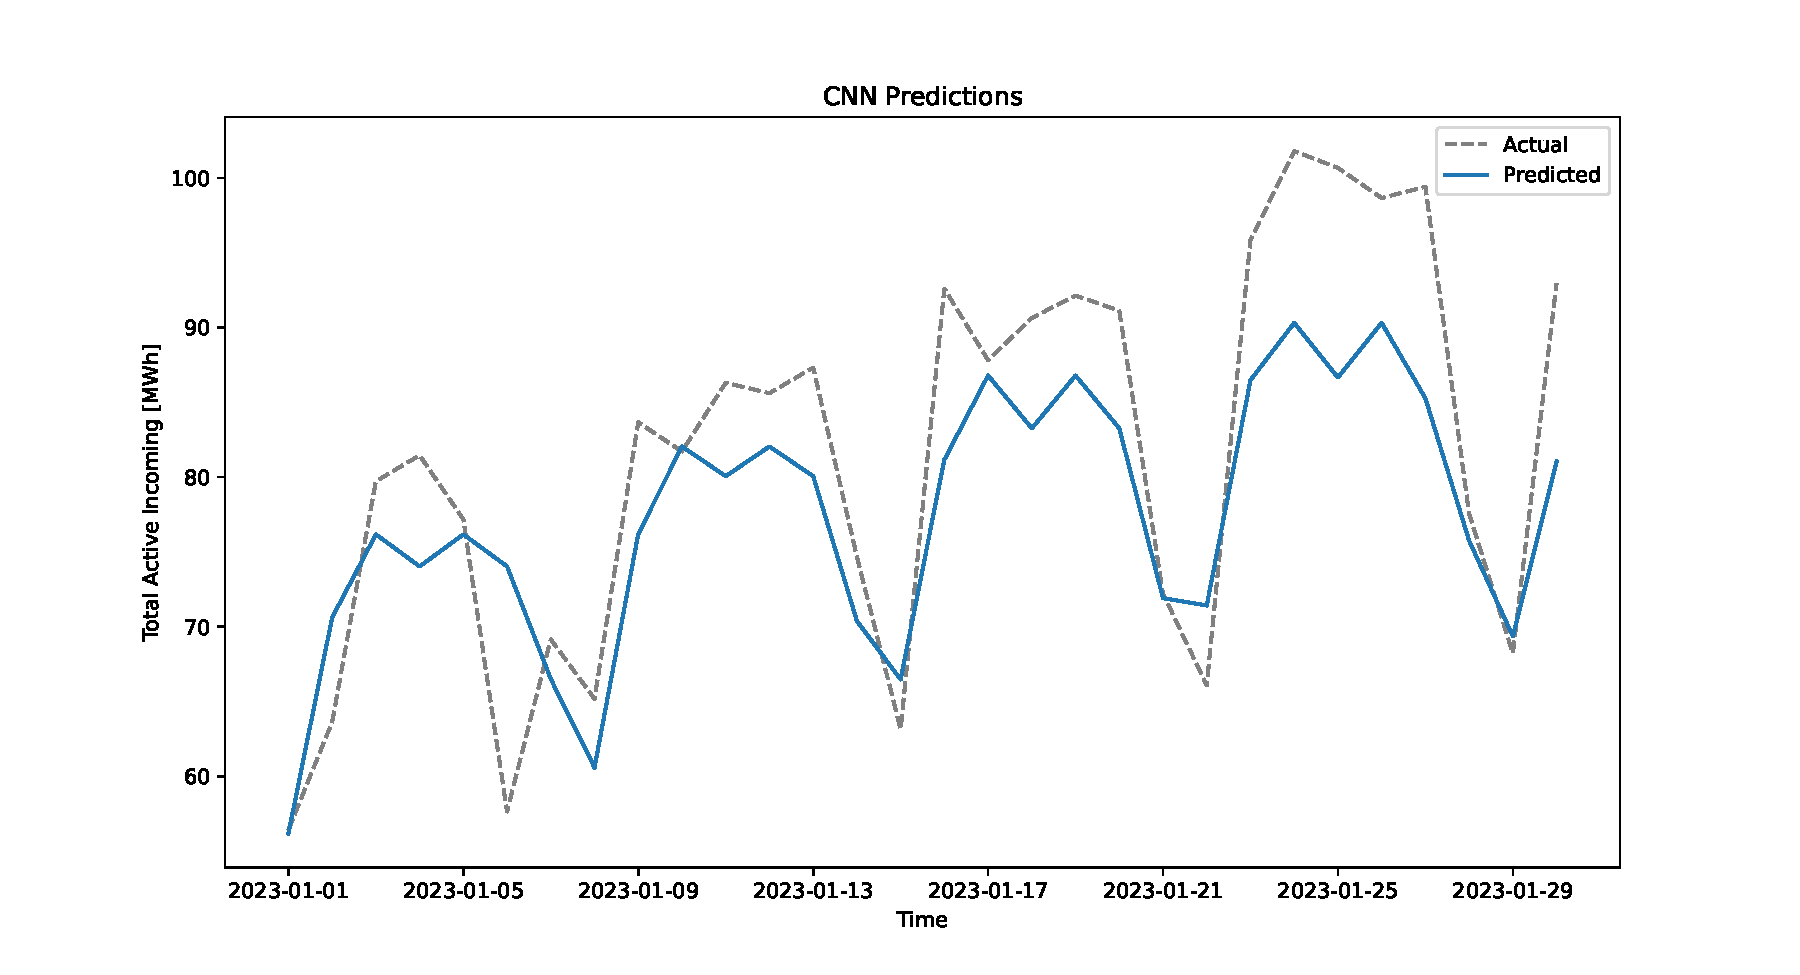
\includegraphics[width=1\textwidth]{images/demand/CNN_daily_aggregated}
\caption{The forecasts produced by the convolutional neural network model for the last split in comparison to the actual values.}
\label{fig:demandcnndailyforecasts}
\end{figure}

\begin{figure}[H]
\centering
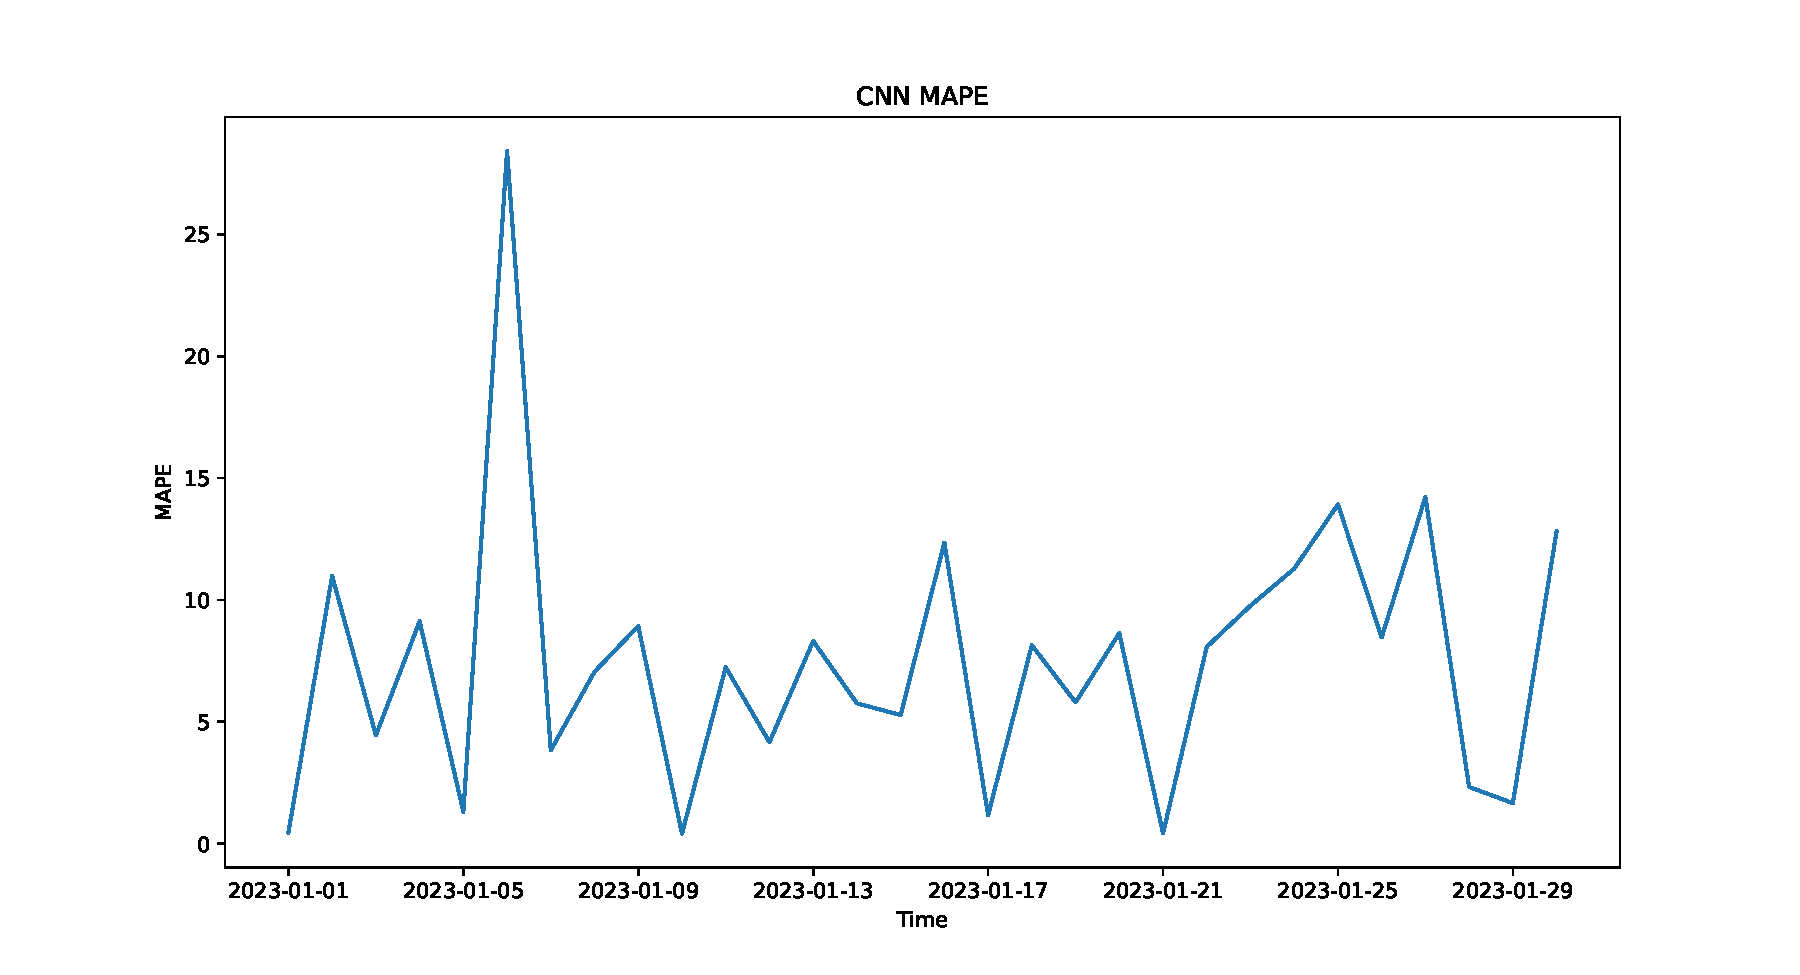
\includegraphics[width=1\textwidth]{images/demand/CNN_daily_aggregated_mape}
\caption{The absolute percentage error of forecasts produced by the convolutional neural network model for the last split in comparison to the actual values.}
\label{fig:demandcnndailyforecastsmape}
\end{figure}

\begin{figure}[H]
\centering
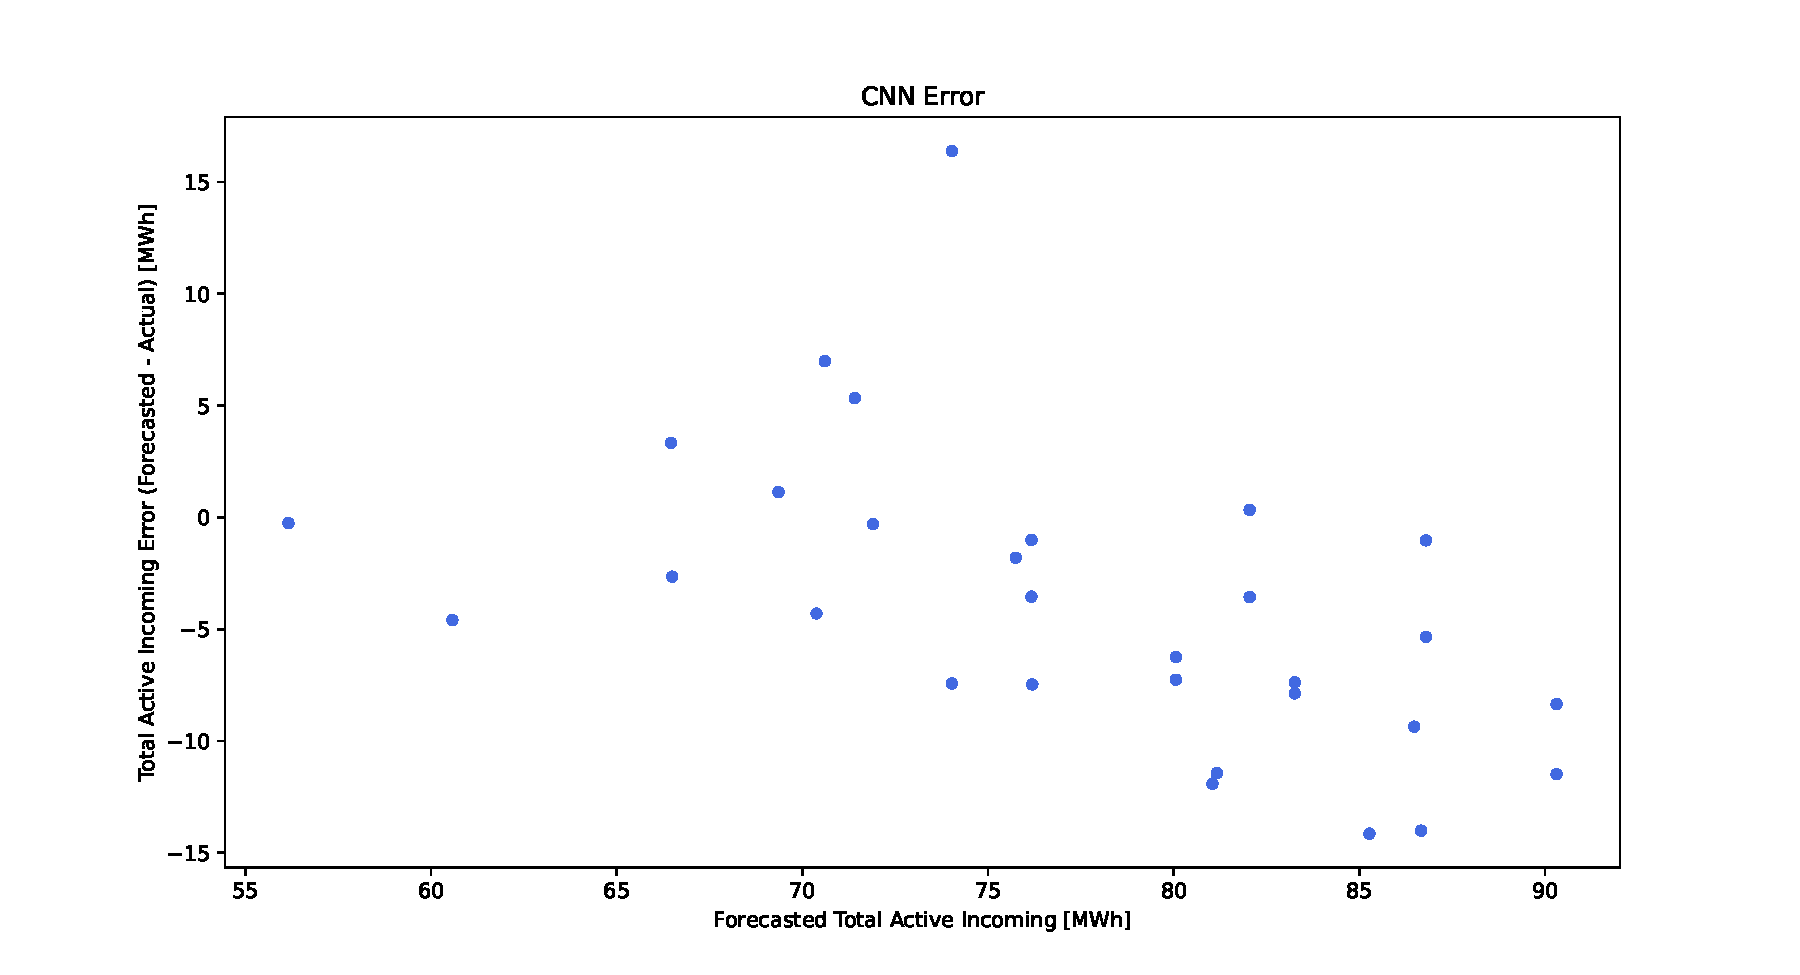
\includegraphics[width=1\textwidth]{images/demand/CNN_error_scatter_plot_predicted_daily_aggregated}
\caption{The scatter plot representing the error of the forecasts produced by the convolutional neural network model for the last split in comparison to the actual values.}
\label{fig:demandcnndailyforecastsscatterplot}
\end{figure}

% TODO then add the comparison with forecasts of their provider
% commentarli (sia il numero che il grafico dell’errore) --> interpretare il dato (perchè è buono?) --> benchmark in letteratura, come va il loro, ecc…
% [valutare criticamente, aspetto tecnologico scientifico]


\section{Electricity production forecasting}
\label{sec:productionval}
\vspace{0.2 cm}

As described in the data preprocessing in chapter~\ref{cha:implementation}, single PV plant production data are aggregated to obtain the aggregated production data over the PV plants.
The target of the predictions is the mean percentage of production, which is calculated as the division of the total produced energy by the total power of the PV plants.
This allows us to have a bounded value from 0 to 100 from which it is possible to obtain the total produced energy simply by multiplying it by the total power of the PV plants.
This was also done since PV plants are added over time and this was unpredictable, this results in predicting the percentage of production of the PV plants.
This data is analyzed to get some descriptive analytics before finding adequate models to forecast the production.
The time series decomposition using an additive model of the hourly percentage of production considering as period of the time series a day is reported in figure~\ref{fig:productiondecomposition}.
It showed a considerable amount of noise, comparable to seasonality and trend in magnitude.
The trend component exhibits a clear peak during the summer season.
As expected, the seasonality component appears to have the most significant impact on the time series.

\begin{figure}[H]
\centering
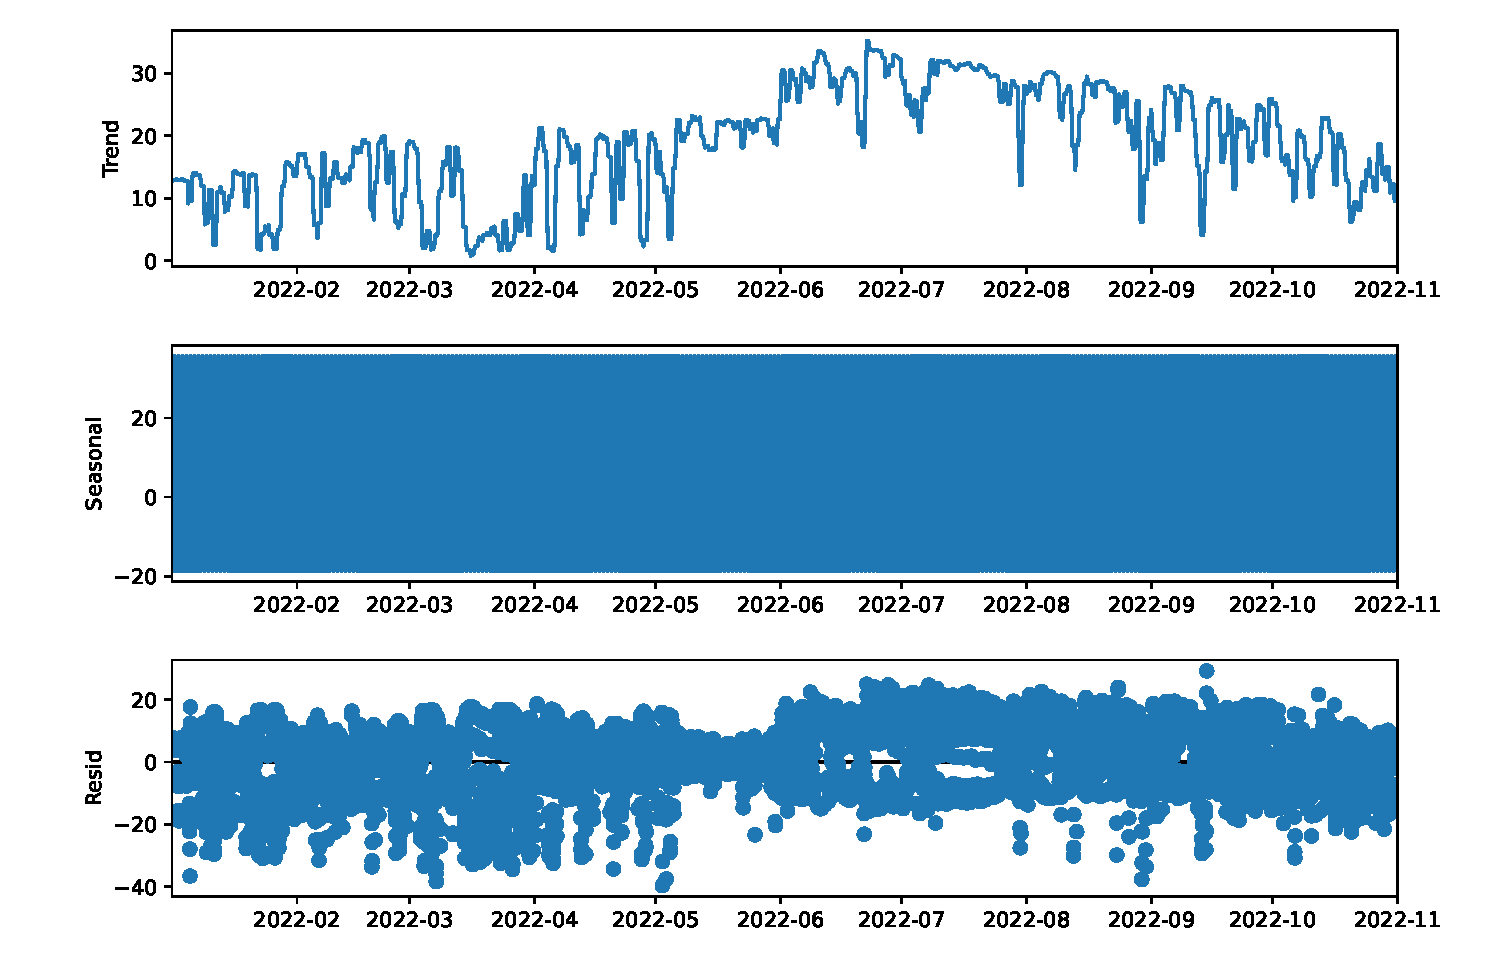
\includegraphics[width=0.5\textwidth]{images/production/hourly_decomposition}
\caption{The time series decomposition of the hourly percentage of production considering as period of the time series a day.}
\label{fig:productiondecomposition}
\end{figure}

The auto-correlation of the hourly percentage of production is reported in figure~\ref{fig:productioncorrelation}.
It shows a high auto-correlation value in the closest time lag and also at every 24 hours, with the value slightly decreasing as the lag increases over days.
This indicates that the production data from the closest time lag and those corresponding to the same hour in the preceding days may be valuable features for predicting a time instant's production.
A reasonable balance can be achieved by incorporating the production data from the past 14 days.

\begin{figure}[H]
\centering
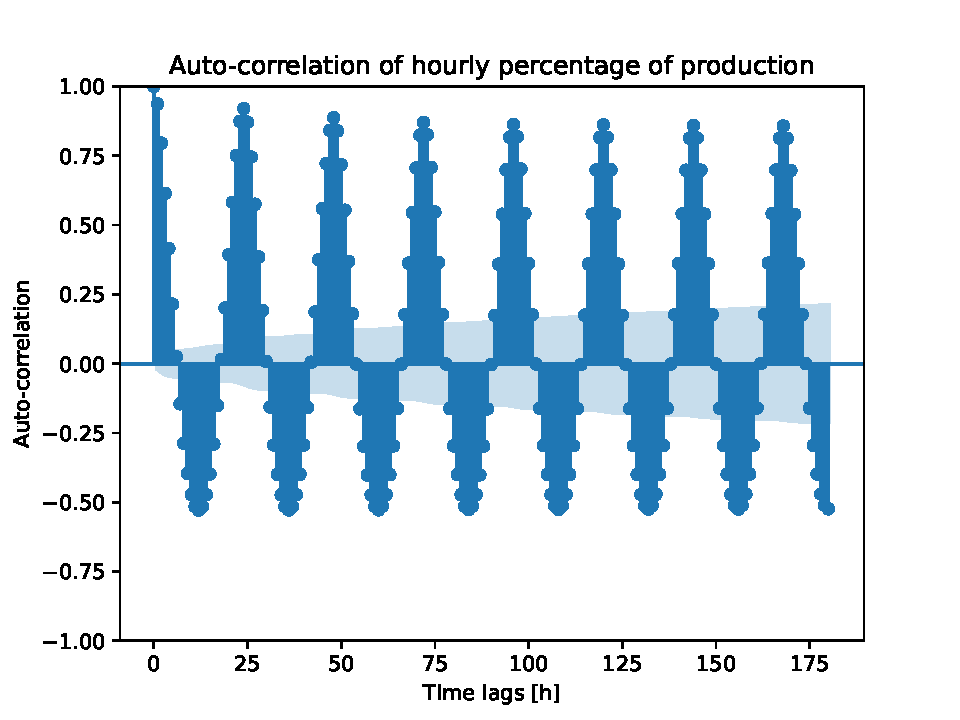
\includegraphics[width=0.4\textwidth]{images/production/hourly_correlation_week_range}
\caption{The auto-correlation of the hourly percentage of production.}
\label{fig:productioncorrelation}
\end{figure}

The coefficients given by the Fourier transform for the hourly percentage of production are reported in figure~\ref{fig:productionft}.
The graphical representation clearly shows a main frequency at the daily periodicity.
Other minor peaks are present mostly at multiples of the 1/day frequency.

\begin{figure}[H]
\centering
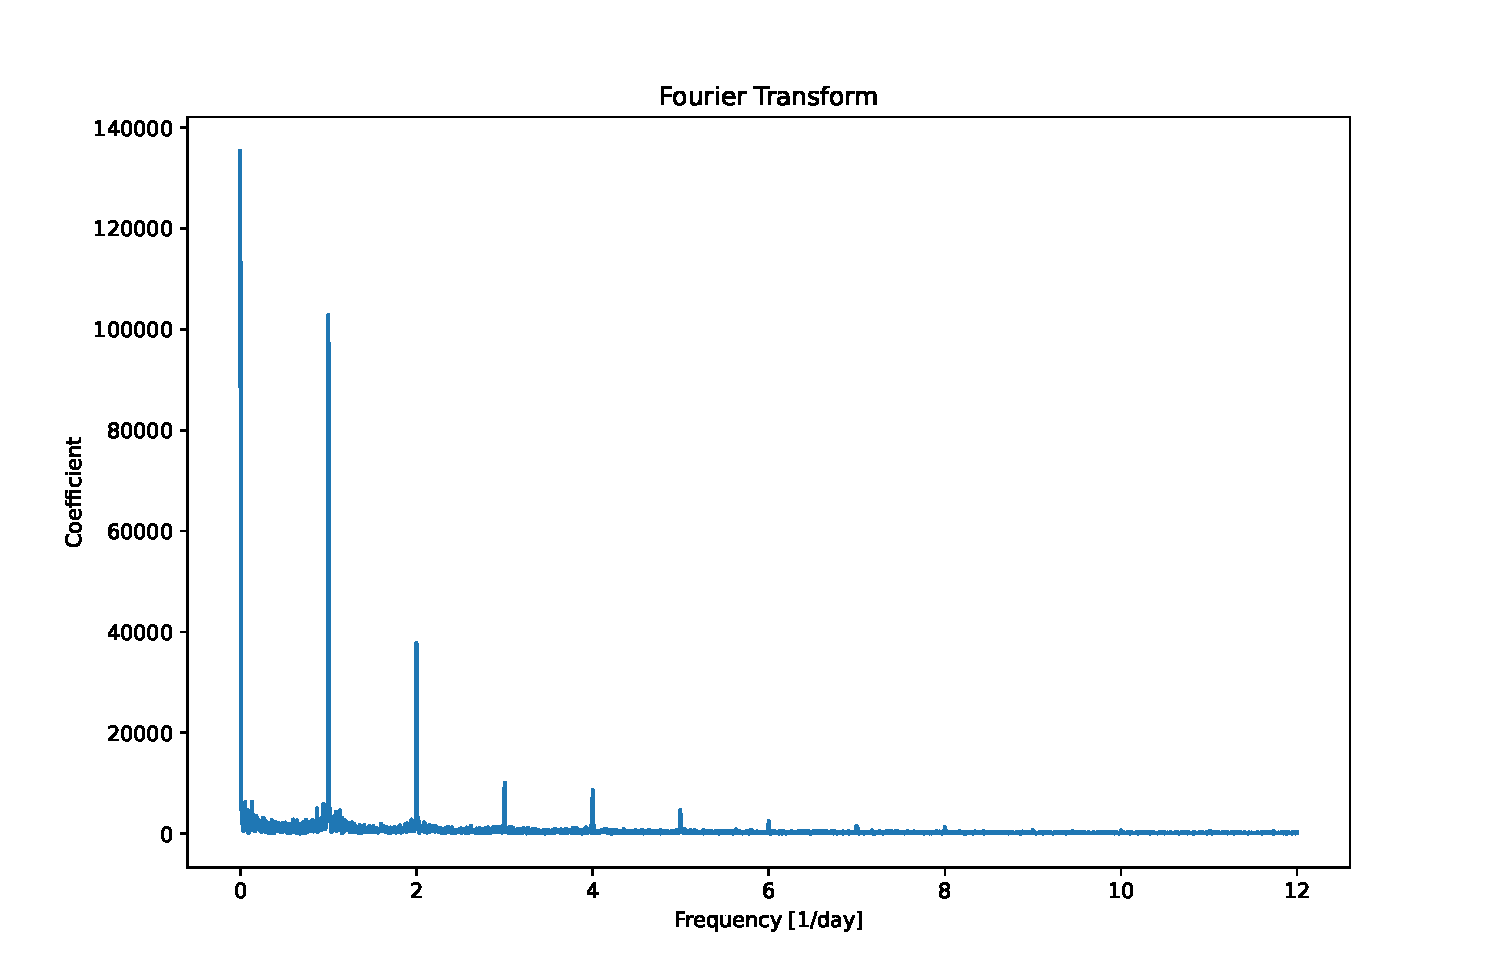
\includegraphics[width=0.4\textwidth]{images/production/ft_hour_day}
\caption{The coefficients given by the Fourier transform for the hourly percentage of production.}
\label{fig:productionft}
\end{figure}

The daily percentage of production is reported in figure~\ref{fig:productiondataplotday}.

\begin{figure}[H]
\centering
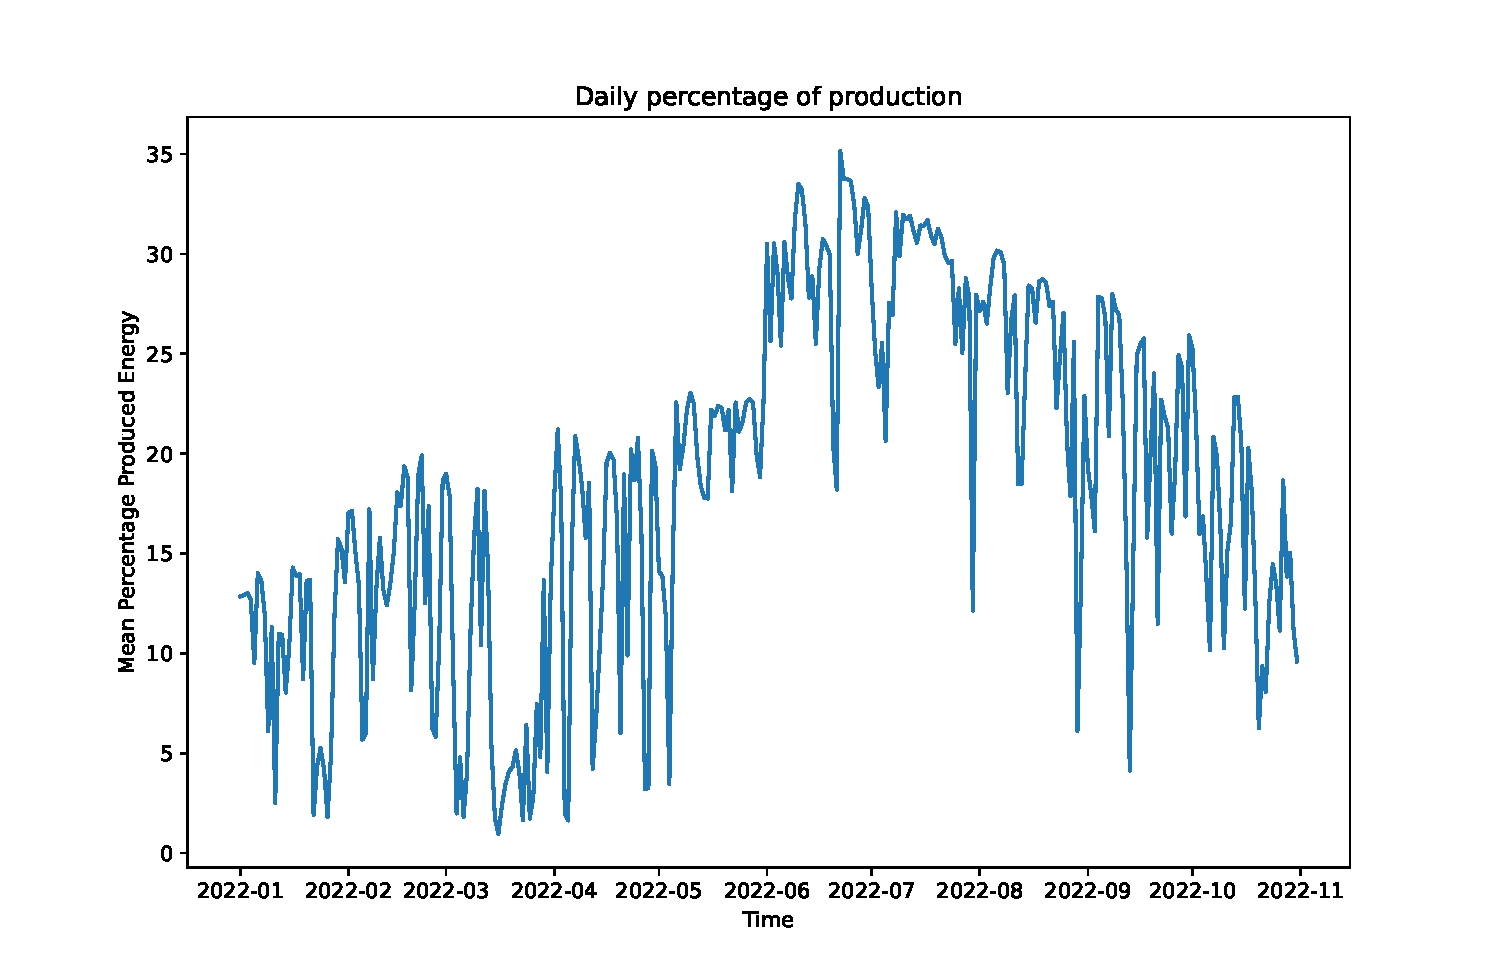
\includegraphics[width=0.5\textwidth]{images/production/data_day_aggregated_plot}
\caption{The daily percentage of production.}
\label{fig:productiondataplotday}
\end{figure}

The time series decomposition using an additive model of the daily percentage of production considering as period of the time series a week is reported in figure~\ref{fig:productiondecompositionday}.
It showed a considerable amount of noise, comparable to the trend in magnitude when not in the summer season.
The trend component exhibits a clear peak during the summer season and appears to be the significant component of the time series.
In this case, considering a weekly period, the seasonality component appears to not have a significant impact on the time series.

\begin{figure}[H]
\centering
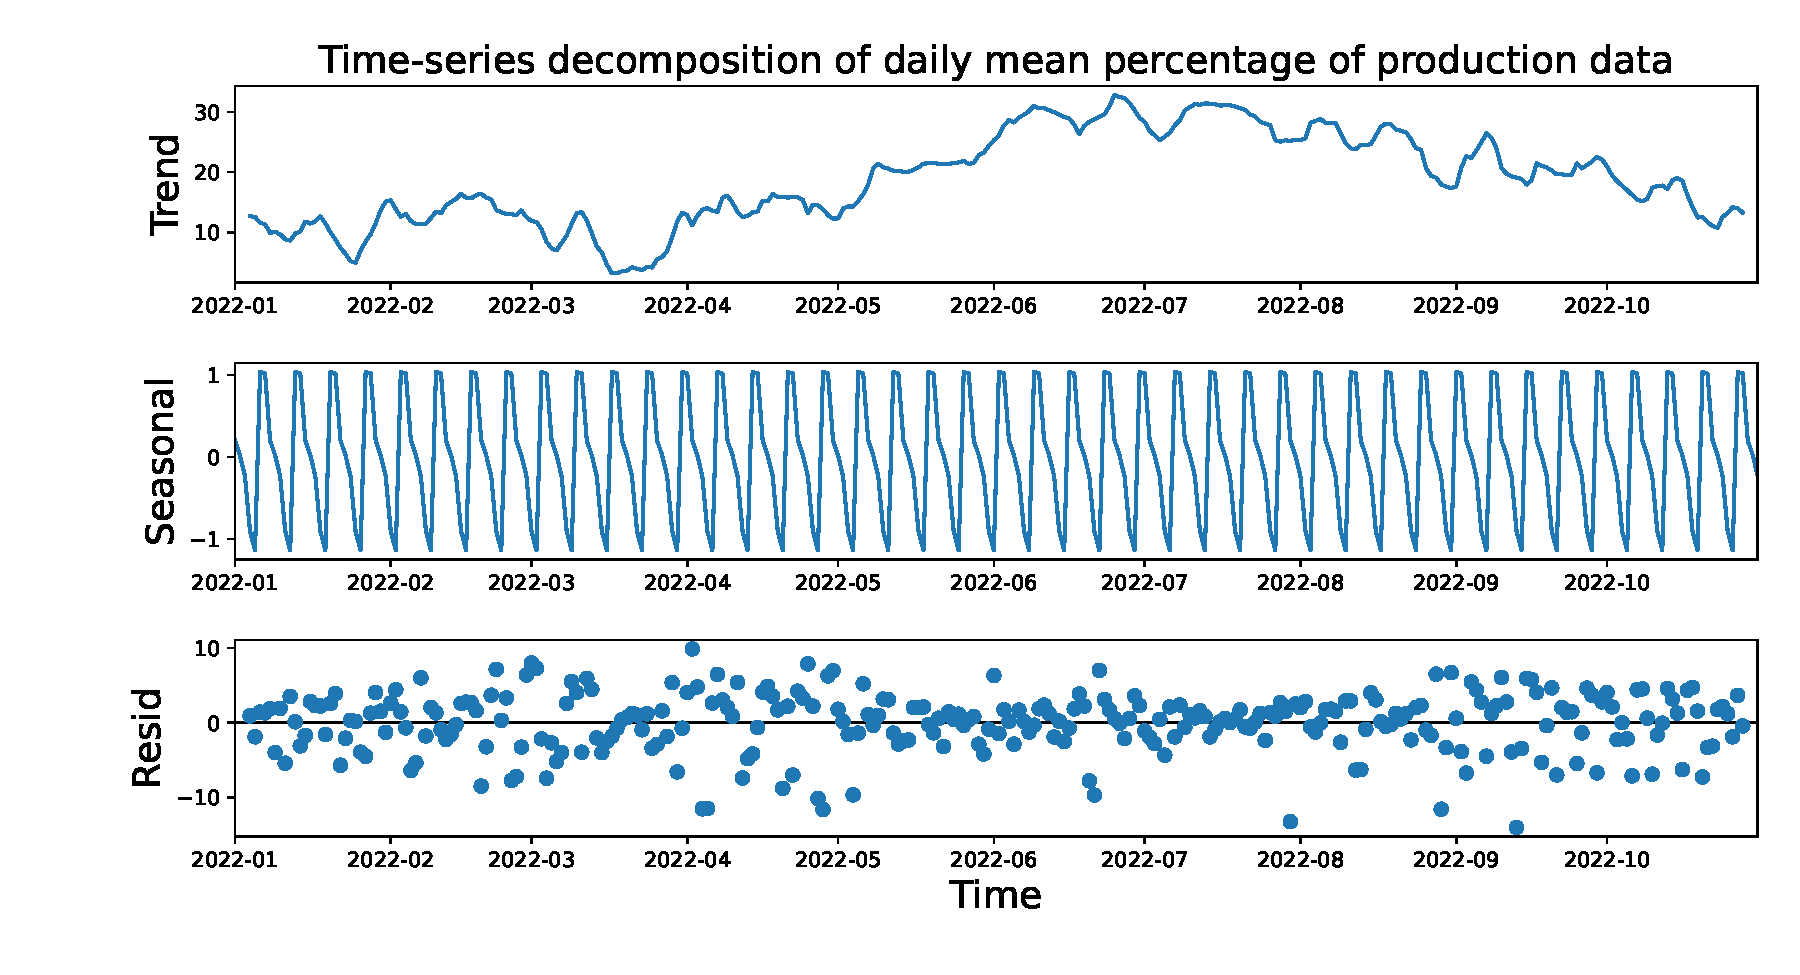
\includegraphics[width=0.5\textwidth]{images/production/daily_aggregated_decomposition}
\caption{The time series decomposition of the daily percentage of production considering as period of the time series a week.}
\label{fig:productiondecompositionday}
\end{figure}

The auto-correlation of the daily percentage of production is reported in figure~\ref{fig:productioncorrelationday}.
It shows a high auto-correlation value in the closest time lag and then a slight decrease as the lag increases over days.

\begin{figure}[H]
\centering
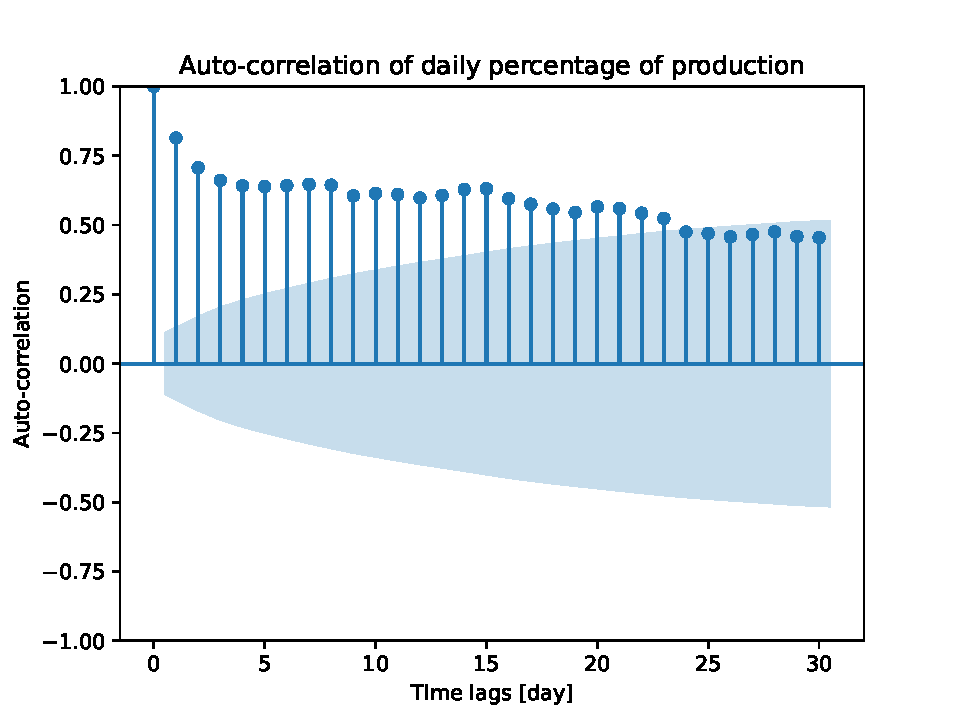
\includegraphics[width=0.4\textwidth]{images/production/daily_aggregated_correlation}
\caption{The auto-correlation of the daily percentage of production.}
\label{fig:productioncorrelationday}
\end{figure}

The coefficients given by the Fourier transform for the daily percentage of production are reported in figure~\ref{fig:productionftday}.
As expected from the time series decomposition, the graphical representation exhibits that there are no main frequencies in the daily percentage of production.

\begin{figure}[H]
\centering
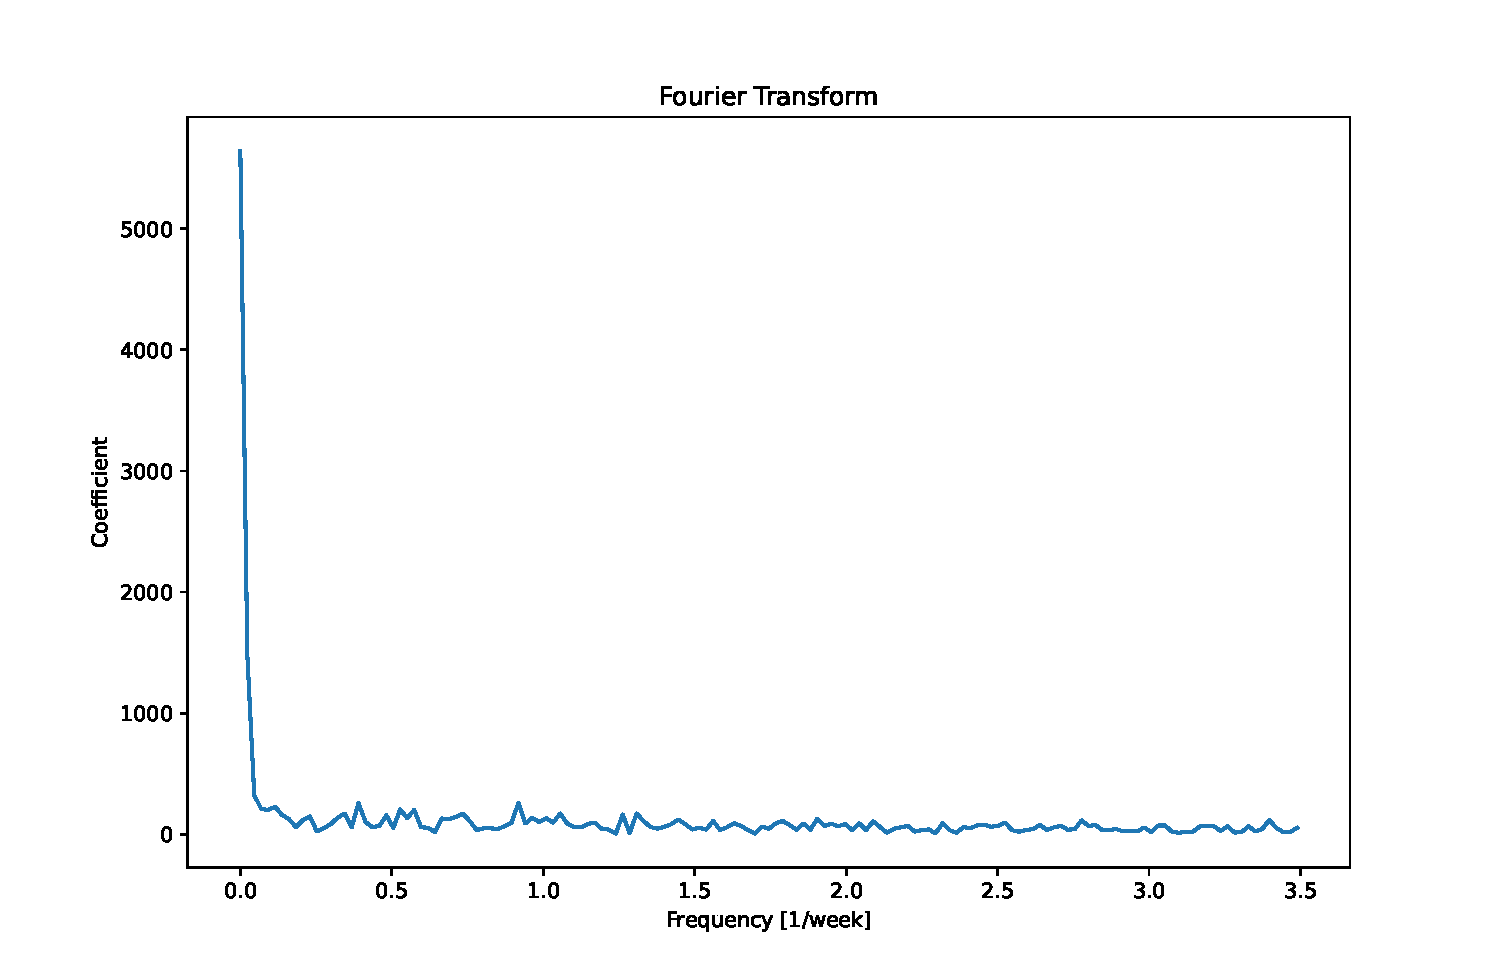
\includegraphics[width=0.4\textwidth]{images/production/ft_day}
\caption{The coefficients given by the Fourier transform for the daily percentage of production.}
\label{fig:productionftday}
\end{figure}

Basic data is enhanced with the air temperature, the apparent temperature, the relative humidity, the wind speed, the wind direction, the pressure altimeter, the visibility, the sky coverage, the diffuse horizontal irradiance, the direct normal irradiance, the global horizontal irradiance, the solar radiation, the UV index, the solar elevation angle, and the solar azimuth angle.
To assess the relationship between these weather variables and the percentage of production, two correlation coefficients were used: Pearson's correlation coefficient and Spearman's rank correlation coefficient.
Pearson's correlation coefficient measures the strength of the linear relationship between two variables, while Spearman's rank correlation coefficient measures the strength of the monotonic relationship.
The pearsonr and spearmanr methods of the SciPy library were used to compute the correlation with weather data.
The results showed that the hourly percentage of production had:
\begin{itemize}
  \item a Pearson correlation coefficient of 0.5621 and a Spearman's rank correlation coefficient of 0.5185 with respect to the air temperature;
  \item a Pearson correlation coefficient of 0.5410 and a Spearman's rank correlation coefficient of 0.5032 with respect to the apparent temperature;
  \item a Pearson correlation coefficient of -0.6318 and a Spearman's rank correlation coefficient of -0.5969 with respect to the relative humidity;
  \item a Pearson correlation coefficient of 0.3105 and a Spearman's rank correlation coefficient of 0.3237 with respect to the wind speed;
  \item a Pearson correlation coefficient of -0.1919 and a Spearman's rank correlation coefficient of -0.2155 with respect to the wind direction;
  \item a Pearson correlation coefficient of -0.2092 and a Spearman's rank correlation coefficient of -0.2645 with respect to the pressure altimeter;
  \item a Pearson correlation coefficient of -0.0132 and a Spearman's rank correlation coefficient of 0.0355 with respect to the visibility;
  \item a Pearson correlation coefficient of -0.2822 and a Spearman's rank correlation coefficient of -0.2375 with respect to the sky coverage;
  \item a Pearson correlation coefficient of 0.8559 and a Spearman's rank correlation coefficient of 0.9340 with respect to the diffuse horizontal irradiance;
  \item a Pearson correlation coefficient of 0.8399 and a Spearman's rank correlation coefficient of 0.9315 with respect to the direct normal irradiance;
  \item a Pearson correlation coefficient of 0.8791 and a Spearman's rank correlation coefficient of 0.9357 with respect to the global horizontal irradiance;
  \item a Pearson correlation coefficient of 0.9073 and a Spearman's rank correlation coefficient of 0.9472 with respect to the solar radiation;
  \item a Pearson correlation coefficient of 0.8571 and a Spearman's rank correlation coefficient of 0.9392 with respect to the UV index;
  \item a Pearson correlation coefficient of 0.8107 and a Spearman's rank correlation coefficient of 0.9057 with respect to the solar elevation angle;
  \item a Pearson correlation coefficient of 0.0450 and a Spearman's rank correlation coefficient of 0.0465 with respect to the solar azimuth angle.
\end{itemize}
It can be noticed that both the coefficients indicate a moderate to strong correlation between the hourly percentage of production and several weather features, including the air temperature, the apparent temperature, the relative humidity, the diffuse horizontal irradiance, the direct normal irradiance, the global horizontal irradiance, the solar radiation, the UV index, and the solar elevation angle.
Therefore, these features are chosen to be incorporated into the prediction models, while the other weather features show weaker correlations and are not considered.

The results showed that the daily percentage of production had:
\begin{itemize}
  \item a Pearson correlation coefficient of 0.7632 and a Spearman's rank correlation coefficient of 0.7721 with respect to the air temperature;
  \item a Pearson correlation coefficient of 0.7434 and a Spearman's rank correlation coefficient of 0.7471 with respect to the apparent temperature;
  \item a Pearson correlation coefficient of -0.7598 and a Spearman's rank correlation coefficient of -0.7474 with respect to the relative humidity;
  \item a Pearson correlation coefficient of 0.1773 and a Spearman's rank correlation coefficient of 0.3769 with respect to the wind speed;
  \item a Pearson correlation coefficient of -0.2405 and a Spearman's rank correlation coefficient of -0.2689 with respect to the wind direction;
  \item a Pearson correlation coefficient of -0.2506 and a Spearman's rank correlation coefficient of -0.2559 with respect to the pressure altimeter;
  \item a Pearson correlation coefficient of 0.2545 and a Spearman's rank correlation coefficient of 0.3259 with respect to the visibility;
  \item a Pearson correlation coefficient of -0.7004 and a Spearman's rank correlation coefficient of -0.6542 with respect to the sky coverage;
  \item a Pearson correlation coefficient of 0.6244 and a Spearman's rank correlation coefficient of 0.6939 with respect to the diffuse horizontal irradiance;
  \item a Pearson correlation coefficient of 0.6216 and a Spearman's rank correlation coefficient of 0.6923 with respect to the direct normal irradiance;
  \item a Pearson correlation coefficient of 0.6305 and a Spearman's rank correlation coefficient of 0.6988 with respect to the global horizontal irradiance;
  \item a Pearson correlation coefficient of 0.7878 and a Spearman's rank correlation coefficient of 0.8013 with respect to the solar radiation;
  \item a Pearson correlation coefficient of 0.8389 and a Spearman's rank correlation coefficient of 0.8680 with respect to the UV index;
  \item a Pearson correlation coefficient of 0.6502 and a Spearman's rank correlation coefficient of 0.7079 with respect to the solar elevation angle;
  \item a Pearson correlation coefficient of 0.1457 and a Spearman's rank correlation coefficient of 0.2813 with respect to the solar azimuth angle.
\end{itemize}
It can be noticed that both the coefficients decreased meaning that the mean weather data over the day is less correlated to the daily percentage of production, compared to the hourly granularity.
Only the hourly granularity is considered since PV plants are highly correlated with weather data and the aggregation over the day loses part of this correlation.

If we were forecasting the production of each PV plant individually, the weather data at the specific locations of the plants would result in a higher correlation with the production data and likely allow the models to produce more accurate forecasts.
However, since we are aggregating the production from multiple PV plants and looking for the overall percentage of production in the hour, using the weather data from a location located in the middle of the PV plants is also acceptable.
In figure~\ref{fig:pvplantsmap}, the locations of the PV plants and of the weather station are reported.

\begin{figure}[H]
\centering
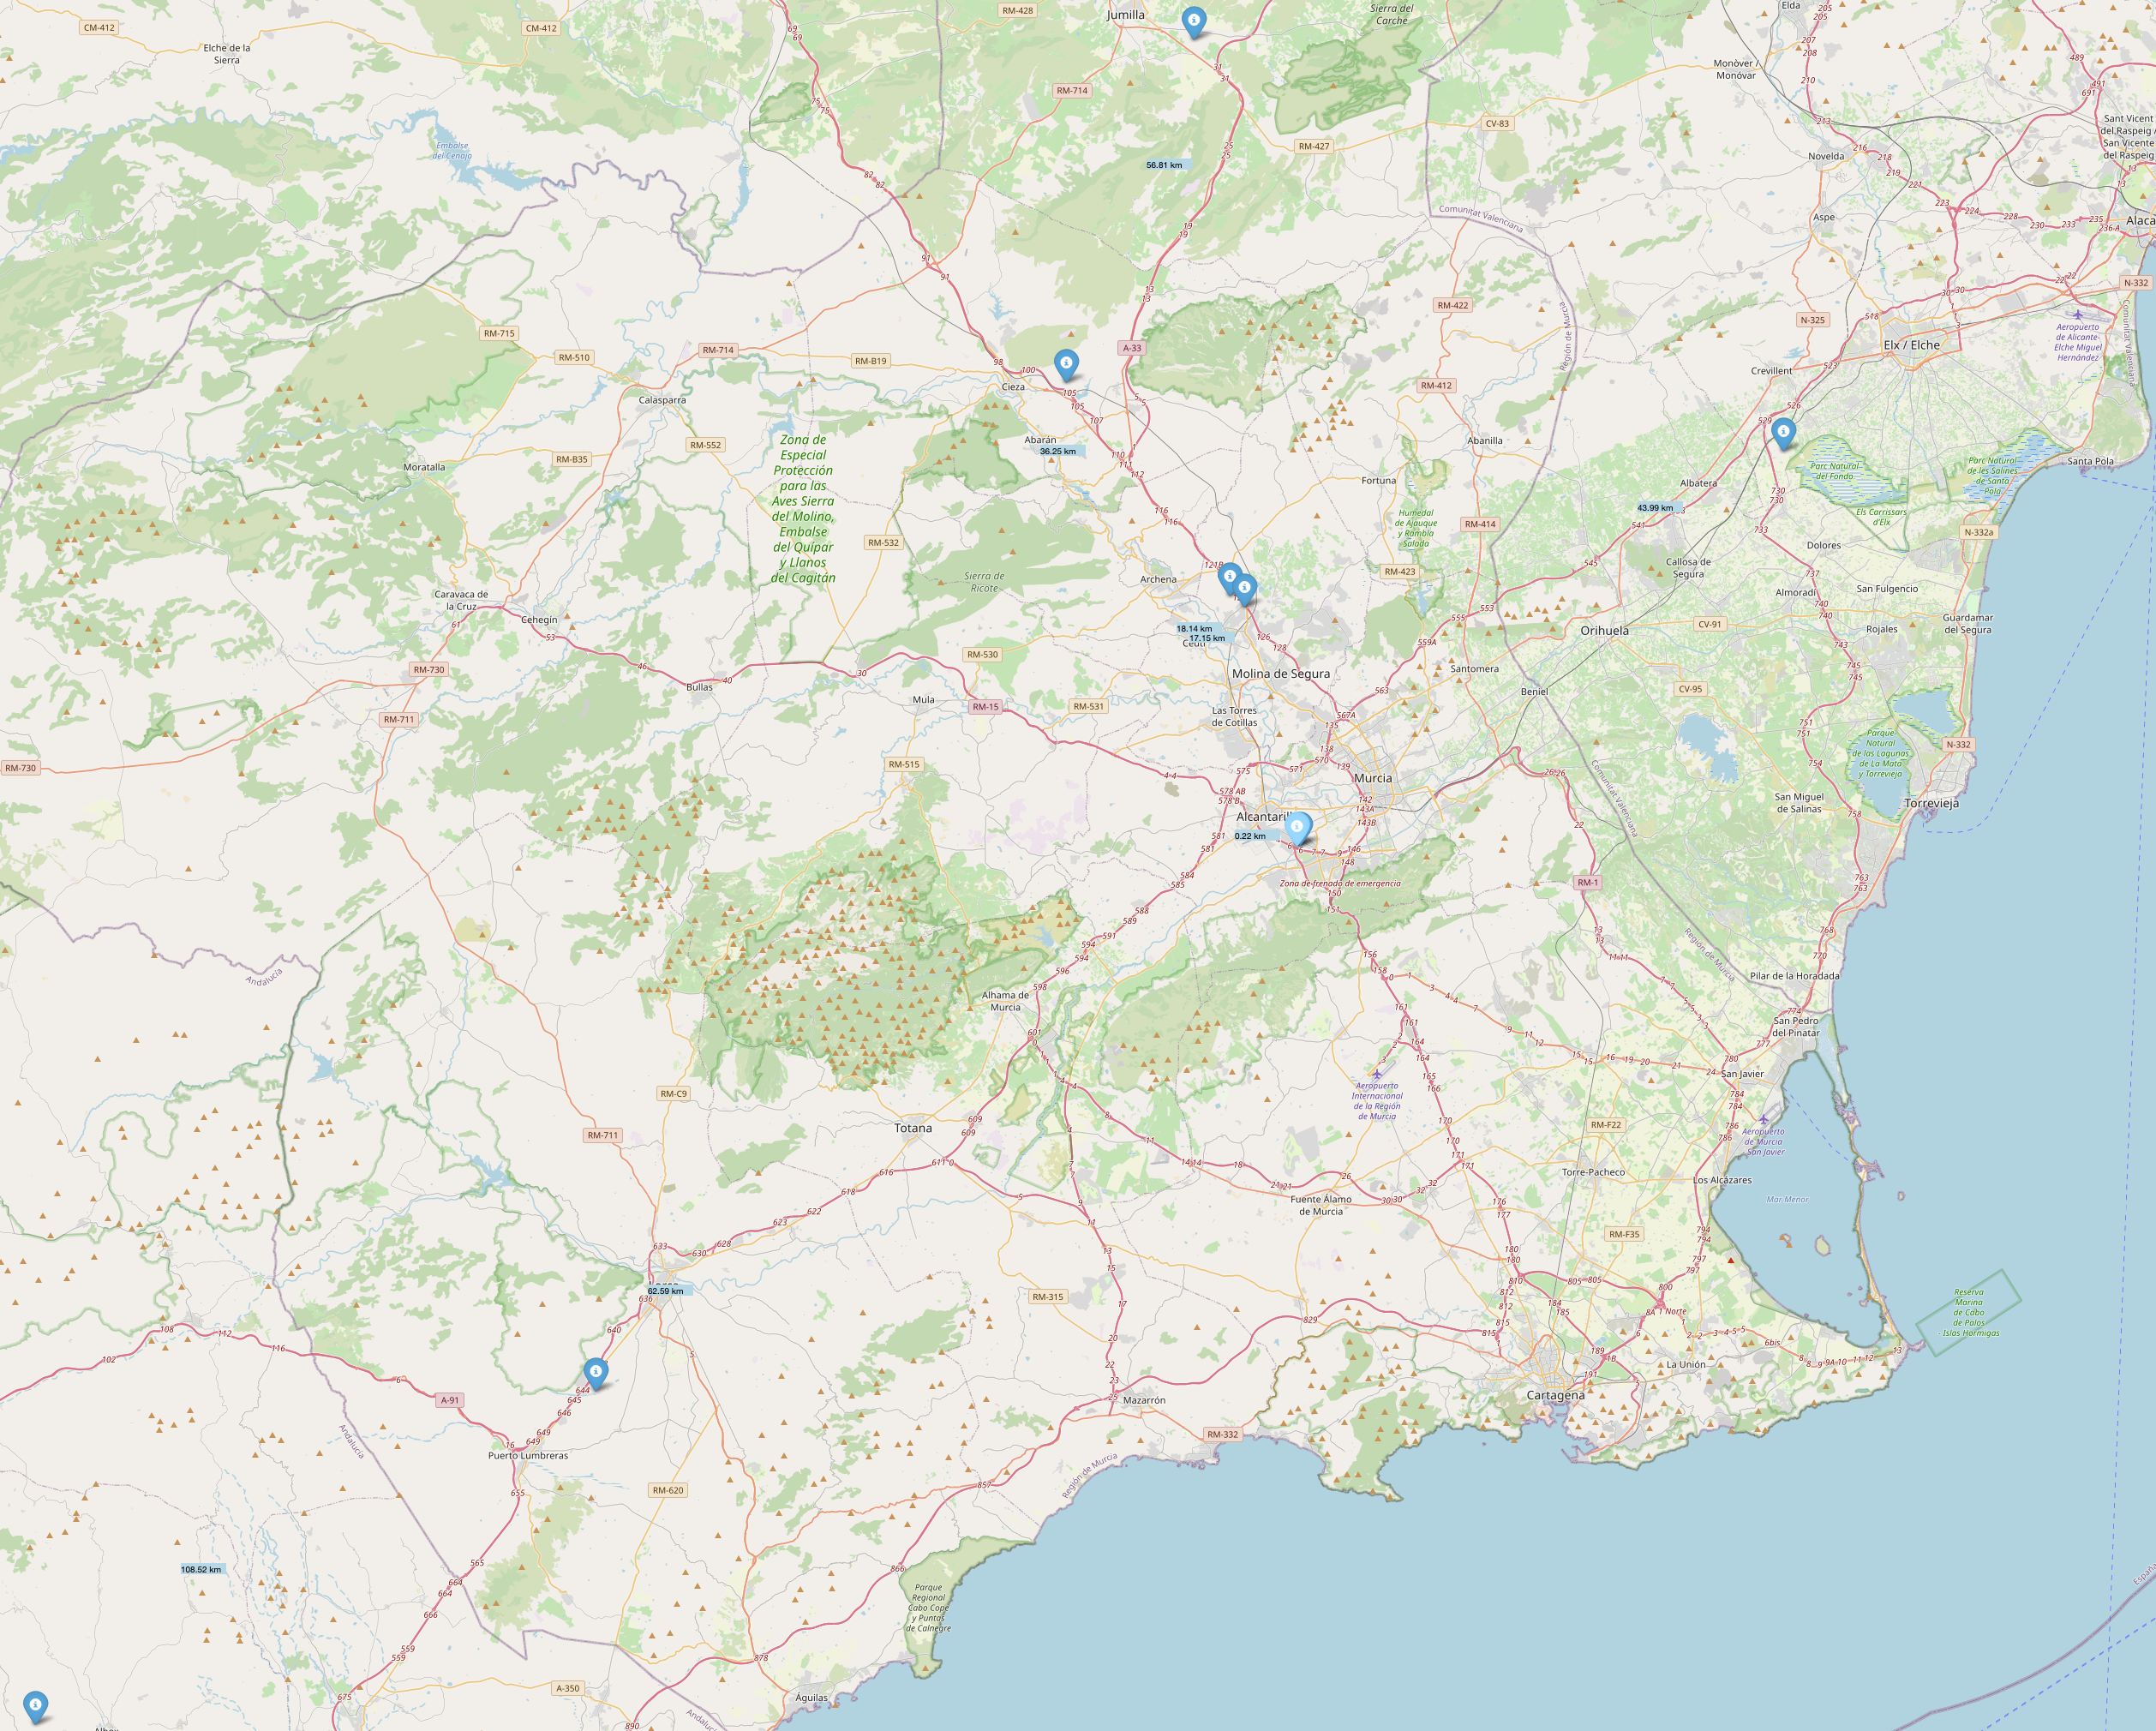
\includegraphics[width=0.8\textwidth]{images/production/pv_plants_map}
\caption{The map of the city of Murcia with indicated the location of the PV plants with a blue icon and of the revelation station with a lightblue icon. The distances between each PV plant and the weather station are reported in lightblue boxes near the PV plant locations.}
\label{fig:pvplantsmap}
\end{figure}

After this data analysis, the specific parameters used in the models can be explained more in detail.
The parameters for the different models were tested and verified on training data to result in the best-performing models, this was done by trying different values and configurations.
The baseline approach is built considering the repetition of past days since data presents a high correlation with that time instant and could lead to a reasonable baseline performance to achieve.
A simple ARIMA model considers the single hours without seasonally on the week period like for demand prediction since data does not present a relevant correlation with that time instants.
The support vector regressor model uses a radial basis function kernel with a configuration of the C parameter (regularization parameter of squared l2 penalty) to 1.0 to penalize the complexity of the model, and the epsilon parameter defining the epsilon-tube for no penalty to 0.1 as a trade-off between accuracy and generalization.
The hist gradient boosting regressor model uses as loss the absolute error.
The learning rate was set to 0.1, 100 estimators were used and l2 regularization was not set.
The parameters for tree definition are 31 as the maximum number of leaves, depth is not constrained, 20 as the minimum number of samples per leaf, and 255 as the maximum number of bins.
For the extreme gradient boosting regressor model, tree-based models were used and the construction algorithm is automatically chosen by heuristic to choose the fastest method.
It uses a squared loss since this was the supported metric closer to our evaluation metric.
The learning rate was set to 0.3, 100 estimators were used and l2 regularization was set with a weight of 1.0.
The parameters for tree definition are 6 as the maximum depth, and the maximum number of leaves is not constrained.
The Prophet model was built keeping the default parameters for automatically detecting seasonalities and best fitting the training data.

The LSTM model was designed as a 2-layer model with 32 Bidirectional LSTM units in the first layer which use ReLU activation function and sigmoid as recurrent activation function with both dropout and recurrent dropout of 0.02.
The second layer is composed of 16 Bidirectional LSTM units which use ReLU activation function and sigmoid as recurrent activation function without dropout and recurrent dropout.
The output of the layer goes inside a dense unit to output the final prediction.
The model is trained using mean absolute error as loss and Nadam as optimizer with a learning rate of 0.005.

The GRU model was designed as a 2-layer model with 32 Bidirectional GRU units in the first layer which use ReLU activation function and sigmoid as recurrent activation function with both dropout and recurrent dropout of 0.02.
Subsequently, the second layer is composed of 16 Bidirectional GRU units which use ReLU activation function and sigmoid as recurrent activation function without dropout and recurrent dropout.
The output of the layer goes inside a dense unit to output the final prediction.
The model is trained using mean absolute error as loss and Nadam as optimizer with a learning rate of 0.005.

The CNN model was designed as a 2-layer model with a first layer composed of 24 1D Convolutional units with a kernel size of 5 which uses ReLU activation function.
A 1D max polling operation is applied before entering the second layer composed of 16 1D Convolutional units with a kernel size of 3 which use ReLU activation function.
A 1D max polling operation is applied before the flattening operation and entering the final dense unit to output the final prediction.
The model is trained using mean absolute error as loss and Nadam as optimizer with a learning rate of 0.005.

The TFT model was configured with 2 LSTM layers with 16 as hidden size, 4 as attention size, and 8 as hidden continuous size.
The dropout is set to 0.02.
The model is trained using mean absolute error as loss and Nadam as optimizer with a learning rate of 0.005.

12 splits were used for block validation with a test size of a week each time, namely 7 days of data.
The models start with 5280 entries as training and predict every time 168 entries until reaching the last prediction instant where the model has a training size of 7128.
The results for hourly granularity are reported in table~\ref{tab:productionhourlyresults}.
Entries are sorted by best MAE using the last split as the test set.
The blocked k-fold cross-validation suggests that the hist gradient boosting regressor model has the best MAE, but looking at the last split this is not confirmed.
In fact, the GRU model performs better on the last split, as the other DL models, this seems to confirm what is seen in demand prediction that with the increase of training data, these models perform better.
It can also be noted that all the models are better than the one-day baseline.
Prophet presents not very good results compared to the other models and is close to the baseline as results on the last split while considering the blocked k-fold cross-validation is the only model that performs worse than it,
In this case, the TFT approach does not seem to perform in an optimal way, and its results are close to the ones of LSTM and ARIMA models.

\begin{table}[H]
\centering
\begin{tabular}{|c|c|c|}
\hline
\textbf{Model} & \textbf{Blocked k-fold} & \textbf{Test on the last split}\\
 & \textbf{cross-validation MAE percentage} & \textbf{MAE percentage}\\
\hline
GRU & 5.70 $\pm$ 1.78 & 2.79\\
\hline
HistGradientBoostingRegressor & 4.16 $\pm$ 0.99 & 2.98\\
\hline
SVR & 5.20 $\pm$ 1.12 & 3.12\\
\hline
CNN & 5.98 $\pm$ 1.52 & 3.27\\
\hline
XGBRegressor & 4.57 $\pm$ 0.97 & 3.42\\
\hline
LSTM & 5.23 $\pm$ 1.46 & 3.51\\
\hline
TFT & 4.70 $\pm$ 1.39 & 3.60\\
\hline
ARIMA & 5.09 $\pm$ 1.35 & 3.64\\
\hline
Prophet & 7.90 $\pm$ 1.62 & 4.38\\
\hline
One Day Baseline & 6.81 $\pm$ 3.14 & 4.58\\
\hline
\end{tabular}
\caption{Table summarizing the results for hourly granularity.}
\label{tab:productionhourlyresults}
\end{table}

The results for hourly granularity at forecasting time on the last time slot including also the combinations of different techniques and the AutoML approach are reported in table~\ref{tab:productionhourlyresultsforecast}.
The combination of the previous techniques was performed by combining one-day baseline and Prophet with possibly one of LSTM, GRU, or CNN with the intent of trying to improve the robustness of DL models with some stable baselines and Prophet model which internally automatically deals with seasonalities, even though for this task it is not performing very well.
The AutoML approach uses the mean MAPE forecasting as loss and it is launched for 10 hours with a maximum function evaluation time of 2 hours.
Also, the mean MAE forecasting was used but provided worse results.
Then the best ensemble of the found models is returned and can be used to forecast.

\begin{table}[H]
\centering
\begin{tabular}{|c|c|c|}
\hline
\textbf{Model} & \textbf{Forecast on the last split}\\
 & \textbf{MAE percentage}\\
\hline
GRU & 2.79\\
\hline
HistGradientBoostingRegressor & 2.86\\
\hline
SVR & 3.12\\
\hline
CNN & 3.27\\
\hline
XGBRegressor & 3.35\\
\hline
LSTM + One Day Baseline & 3.37\\
\hline
GRU + One Day Baseline & 3.45\\
\hline
CNN + One Day Baseline & 3.48\\
\hline
LSTM & 3.51\\
\hline
TFT & 3.60\\
\hline
LSTM + One Day Baseline + Prophet & 3.60\\
\hline
ARIMA & 3.64\\
\hline
CNN + One Day Baseline + Prophet & 3.67\\
\hline
GRU + One Day Baseline + Prophet & 3.70\\
\hline
One Day Baseline + Prophet & 4.38\\
\hline
Prophet & 4.38\\
\hline
One Day Baseline & 4.58\\
\hline
AutoML & 5.89\\
\hline
\end{tabular}
\caption{Table summarizing the results for hourly granularity at forecasting time.}
\label{tab:productionhourlyresultsforecast}
\end{table}

\begin{figure}[H]
\centering
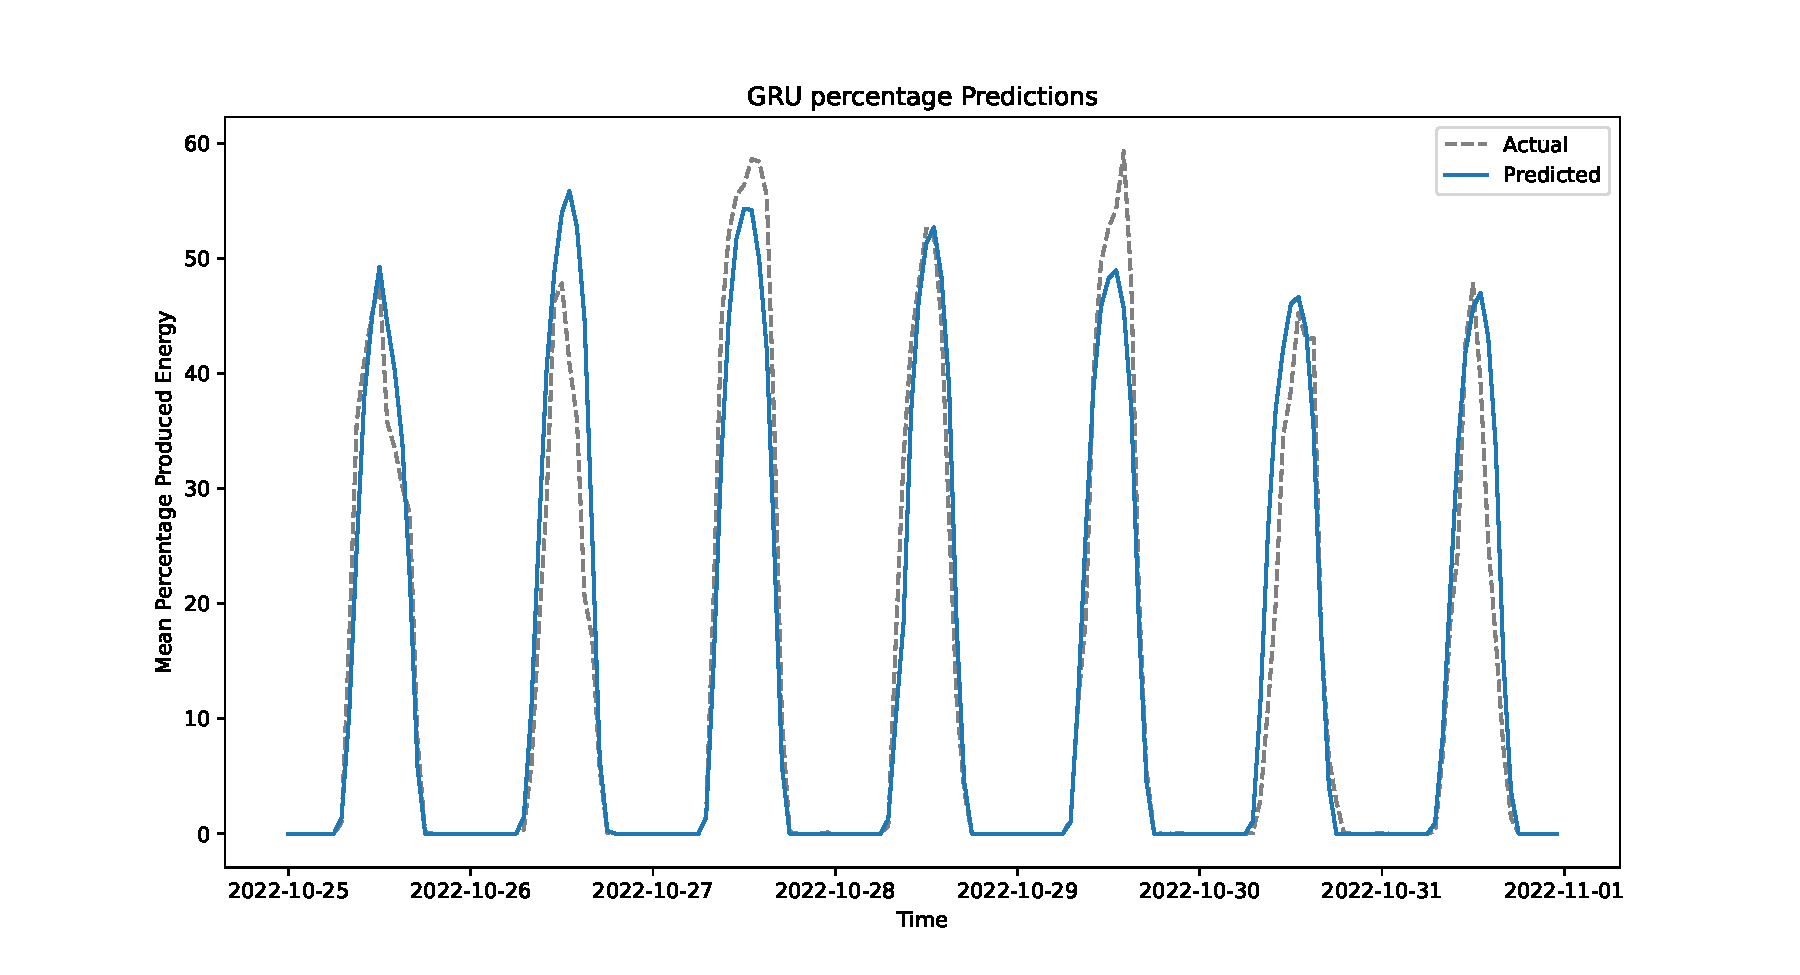
\includegraphics[width=1\textwidth]{images/production/GRU_percentage}
\caption{The forecasts produced by the gated recurrent unit model for the last split in comparison to the actual values.}
\label{fig:productiongruhourlyforecasts}
\end{figure}

Including also combinations and AutoML, there are a few observations that can be done.
The combinations of DL models and the one-week baseline are the most beneficial, but just in the case of LSTM there is an improvement and it is very marginal.
Probably in this case since the baseline and prophet are not well-performing models they are not bringing any significant improvement or robustness to the DL models.
Nonetheless, it might still make sense to investigate the concept of ensemble learning further and optimize this combination at training time to possibly have stronger results at forecasting time.
In this case, AutoML is not able to achieve very good results compared to many other models.
It still has great potential as demonstrated in demand prediction and potentially providing more total training time it can be able to reach better performance.

\begin{figure}[H]
\centering
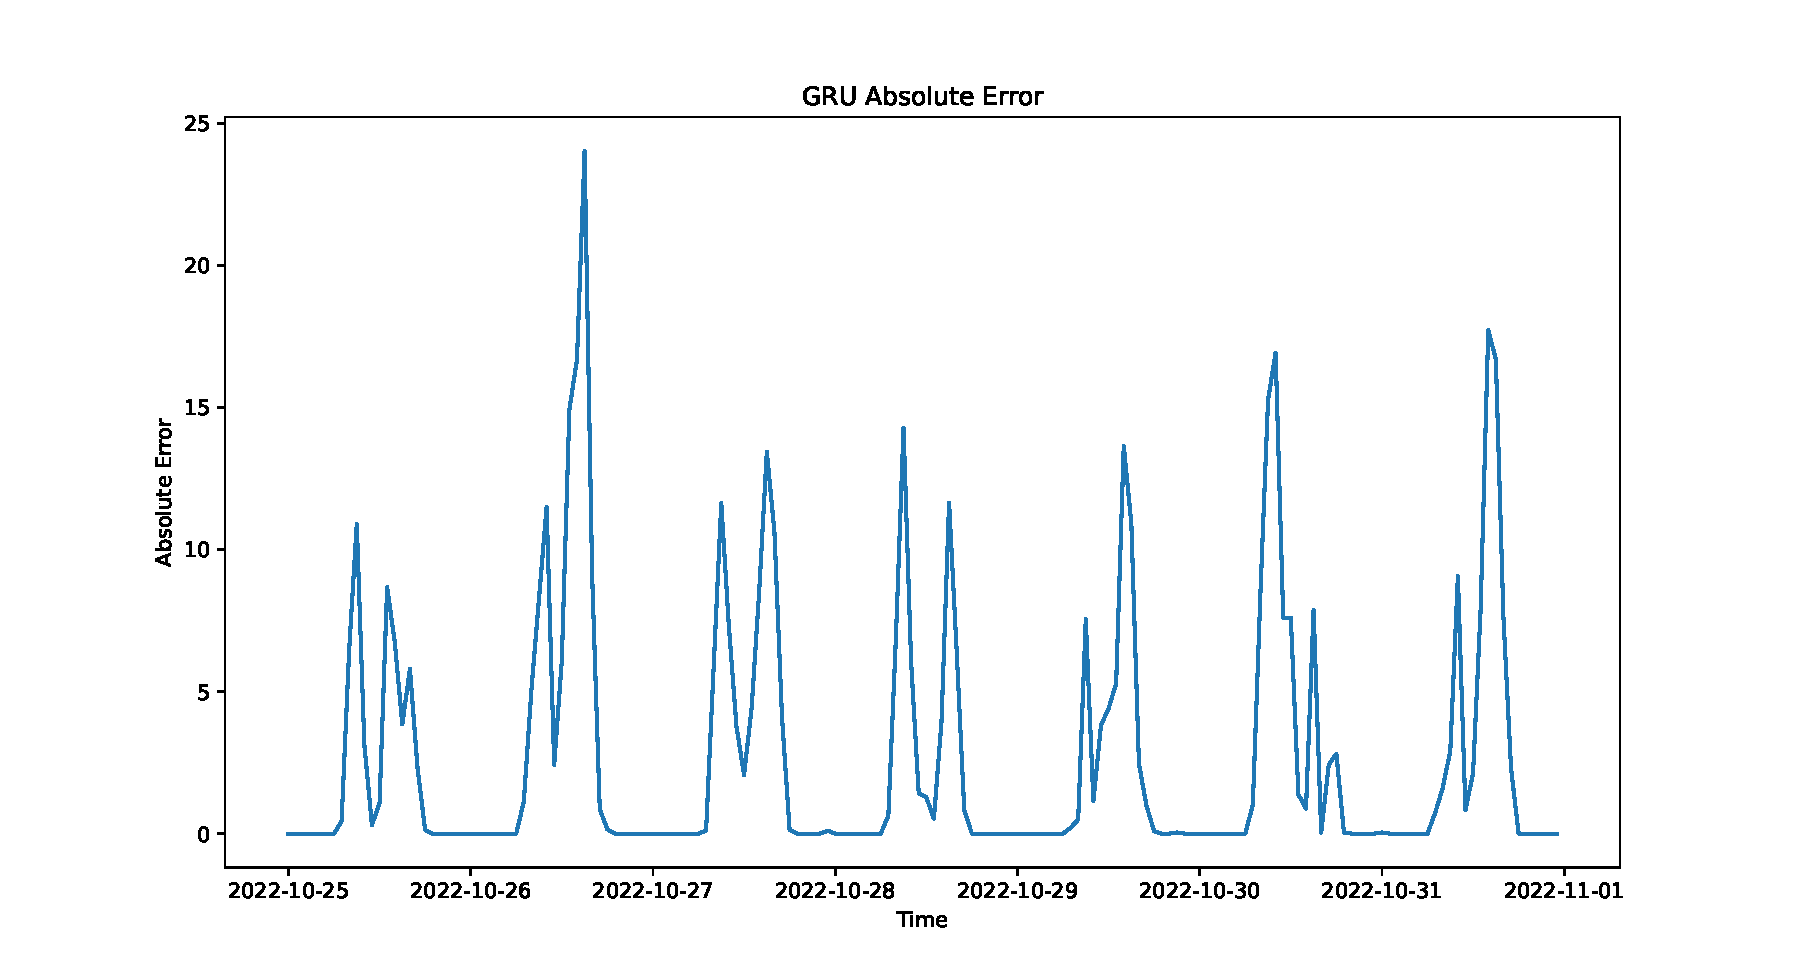
\includegraphics[width=1\textwidth]{images/production/GRU_percentage_mae}
\caption{The absolute error of forecasts produced by the gated recurrent unit model for the last split in comparison to the actual values.}
\label{fig:productiongruhourlyforecastsmae}
\end{figure}

\begin{figure}[H]
\centering
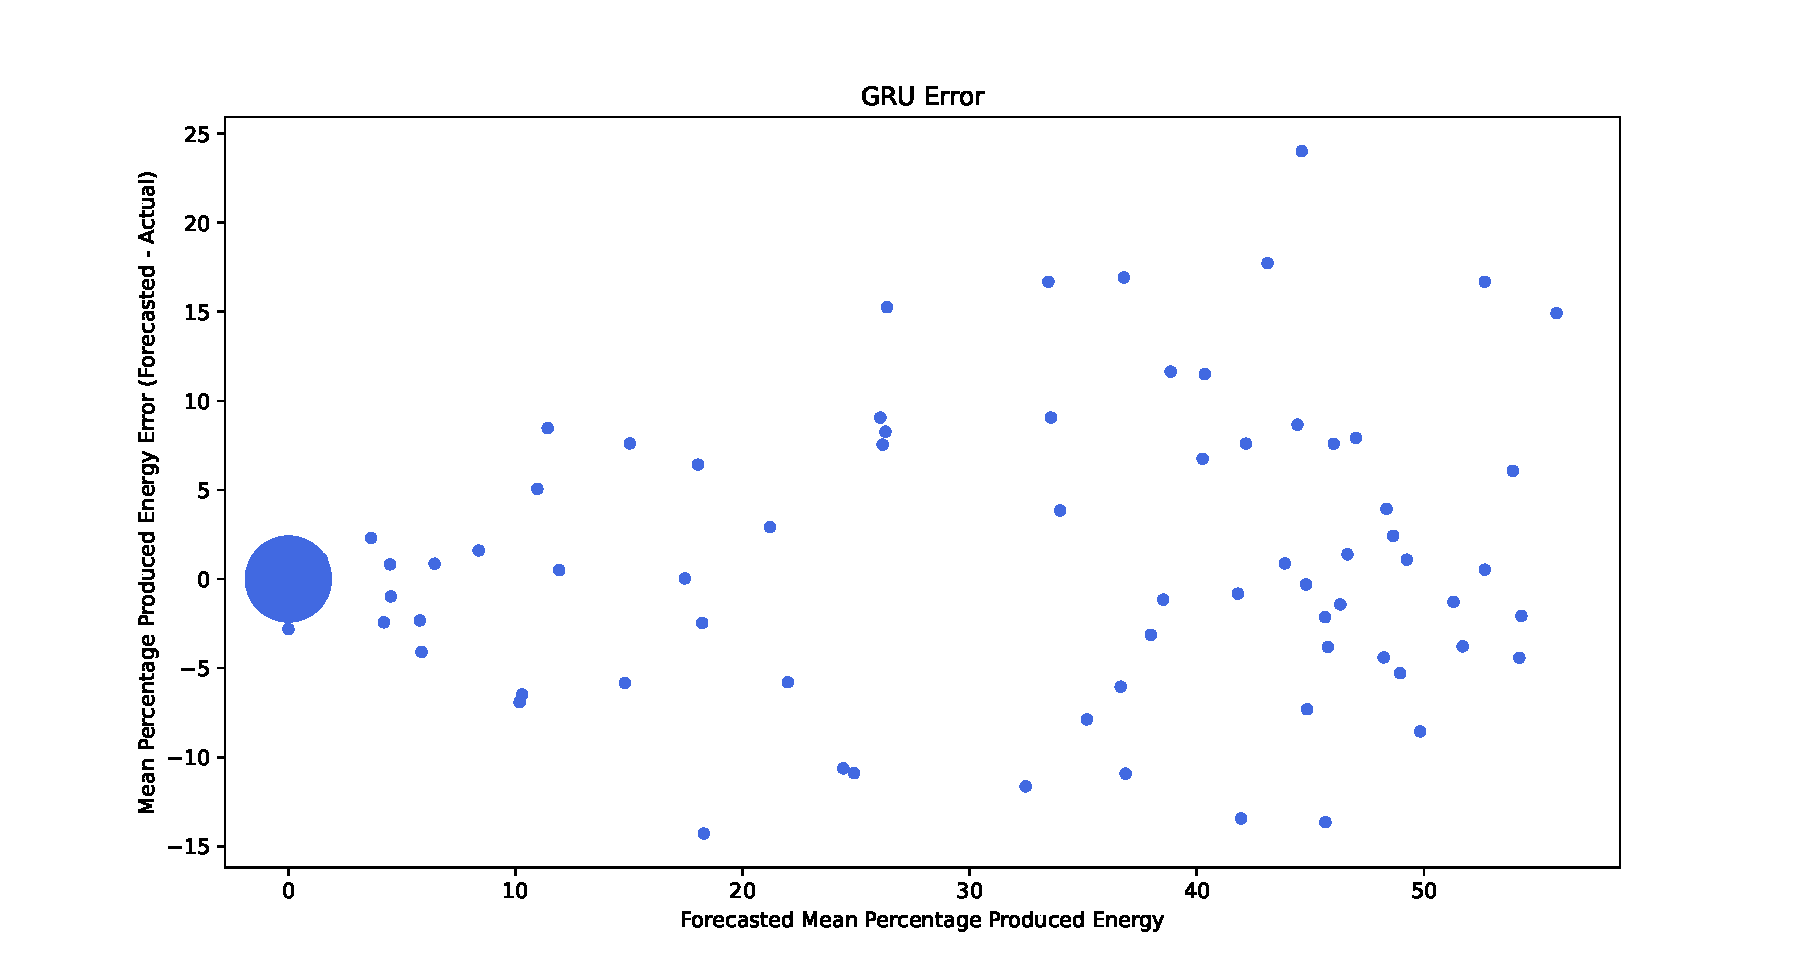
\includegraphics[width=1\textwidth]{images/production/GRU_percentage_error_scatter_plot_predicted}
\caption{The scatter plot representing the error of the forecasts produced by the gated recurrent unit model for the last split in comparison to the actual values.}
\label{fig:productiongruhourlyforecastsscatterplot}
\end{figure}

The forecasts produced by the GRU model for the last split in comparison to the actual values are reported in figure~\ref{fig:productiongruhourlyforecasts}.
It can be noticed that it follows very accurately the signal for most of the test days, for 2 days it underestimates and for one overestimates the actual data.
The absolute error of forecasts produced by the GRU model for the last split in comparison to the actual values is reported in figure~\ref{fig:productiongruhourlyforecastsmae}.
It can be shown that, except for the peak when it overestimates the actual data and some other minor peaks, the error stays below 10\%.
Finally, the scatter plot representing the error of the forecasts produced by the GRU model for the last split in comparison to the actual values is reported in figure~\ref{fig:productiongruhourlyforecastsscatterplot}.
This scatter plot demonstrates that there is no bias and can be also noticed that when the predicted values are low also the error is limited, while when the prediction is high there are both high positive and negative errors.

% TODO then add the comparison with forecasts of their provider
% commentarli (sia il numero che il grafico dell’errore) --> interpretare il dato (perchè è buono?) --> benchmark in letteratura, come va il loro, ecc…
% [valutare criticamente, aspetto tecnologico scientifico]


\section{Consumption baseline forecasting} 
\label{sec:baselineval}
\vspace{0.2 cm}

The consumption data of the three customers are analyzed to get some descriptive analytics before finding adequate models to forecast the consumption baseline of each customer.
The time series decompositions using an additive model of the hourly consumption of the three customers considering as period of the time series a week are reported in figure~\ref{fig:decompositioncustomer1}, figure~\ref{fig:decompositioncustomer2}, and figure~\ref{fig:decompositioncustomer3}.
All three decompositions show a considerable amount of noise, which is dominant in magnitude compared to the trend and seasonality.
For all the customers the seasonal component appears to not have a significant impact on the time series, with the exception of the second customer for which it is twice high in magnitude with respect to the others.
The trend component has a slight impact, for the first customer it is possible to see a peak in the winter, for the second customer it is present a peak in April, and for the third customer there is not a clear trend.

\begin{figure}[H]
\begin{minipage}[b]{8.5cm}
\centering
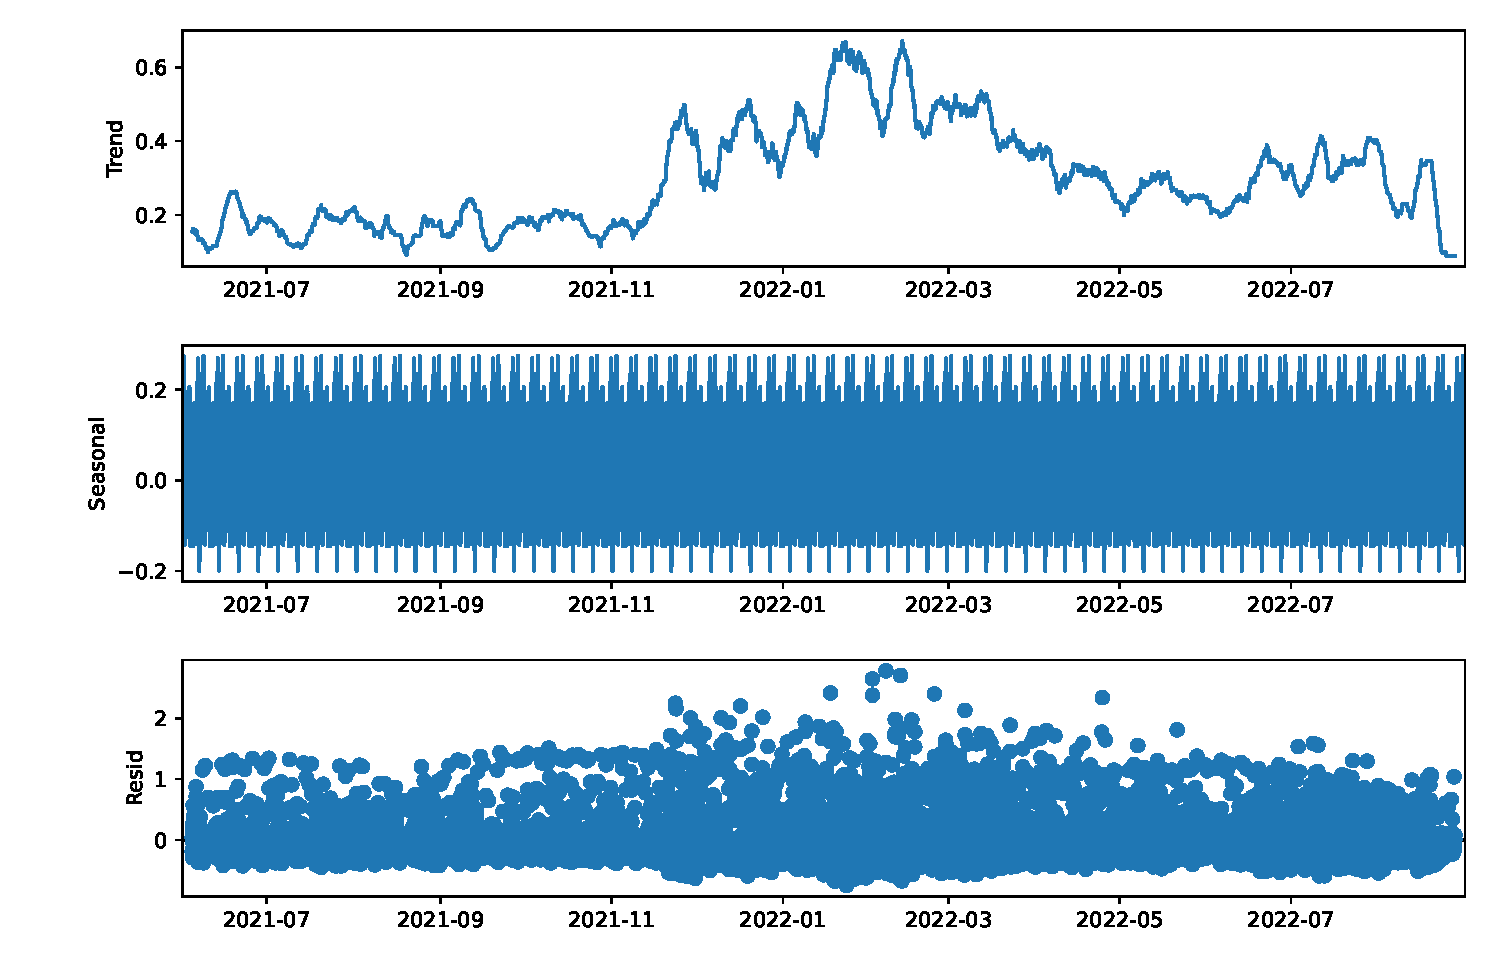
\includegraphics[width=1\textwidth]{images/baseline/hourly_decomposition_week_period_customer1}
\subcaption{First customer.}
\label{fig:decompositioncustomer1}
\end{minipage}
\ \hspace{2mm} \
\begin{minipage}[b]{8.5cm}
\centering
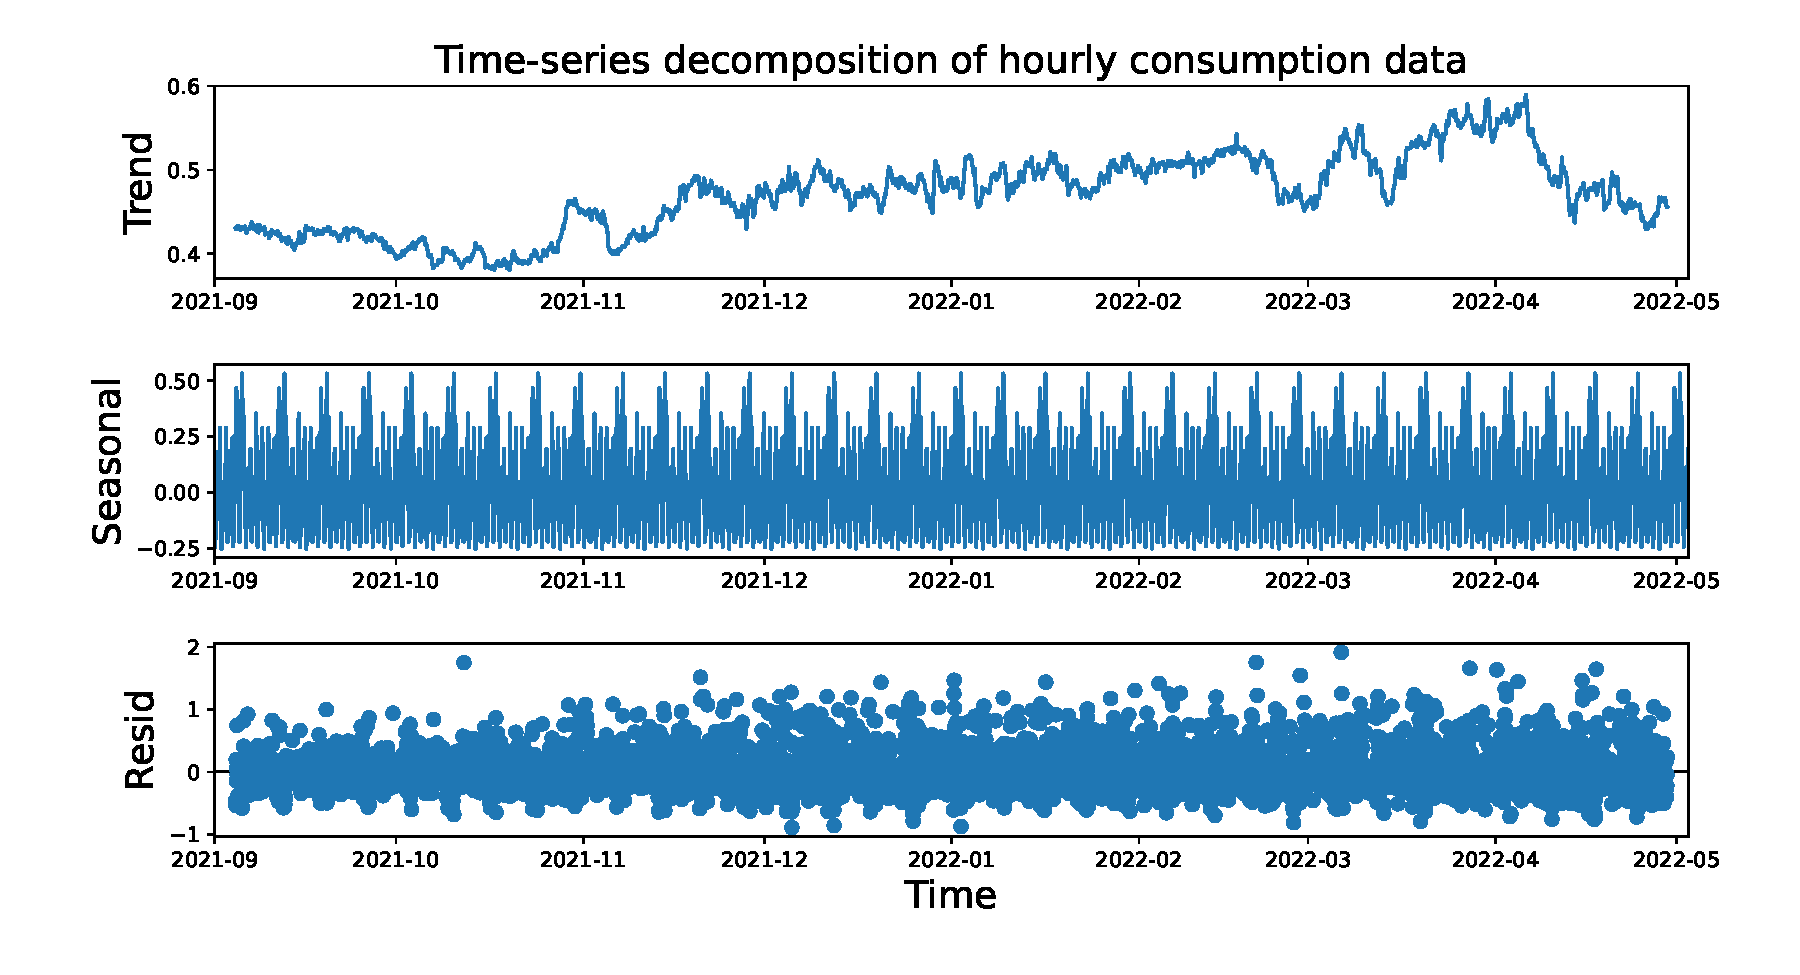
\includegraphics[width=1\textwidth]{images/baseline/hourly_decomposition_week_period_customer2}
\subcaption{Second customer.}
\label{fig:decompositioncustomer2}
\end{minipage}
\begin{minipage}[b]{17cm}
\centering
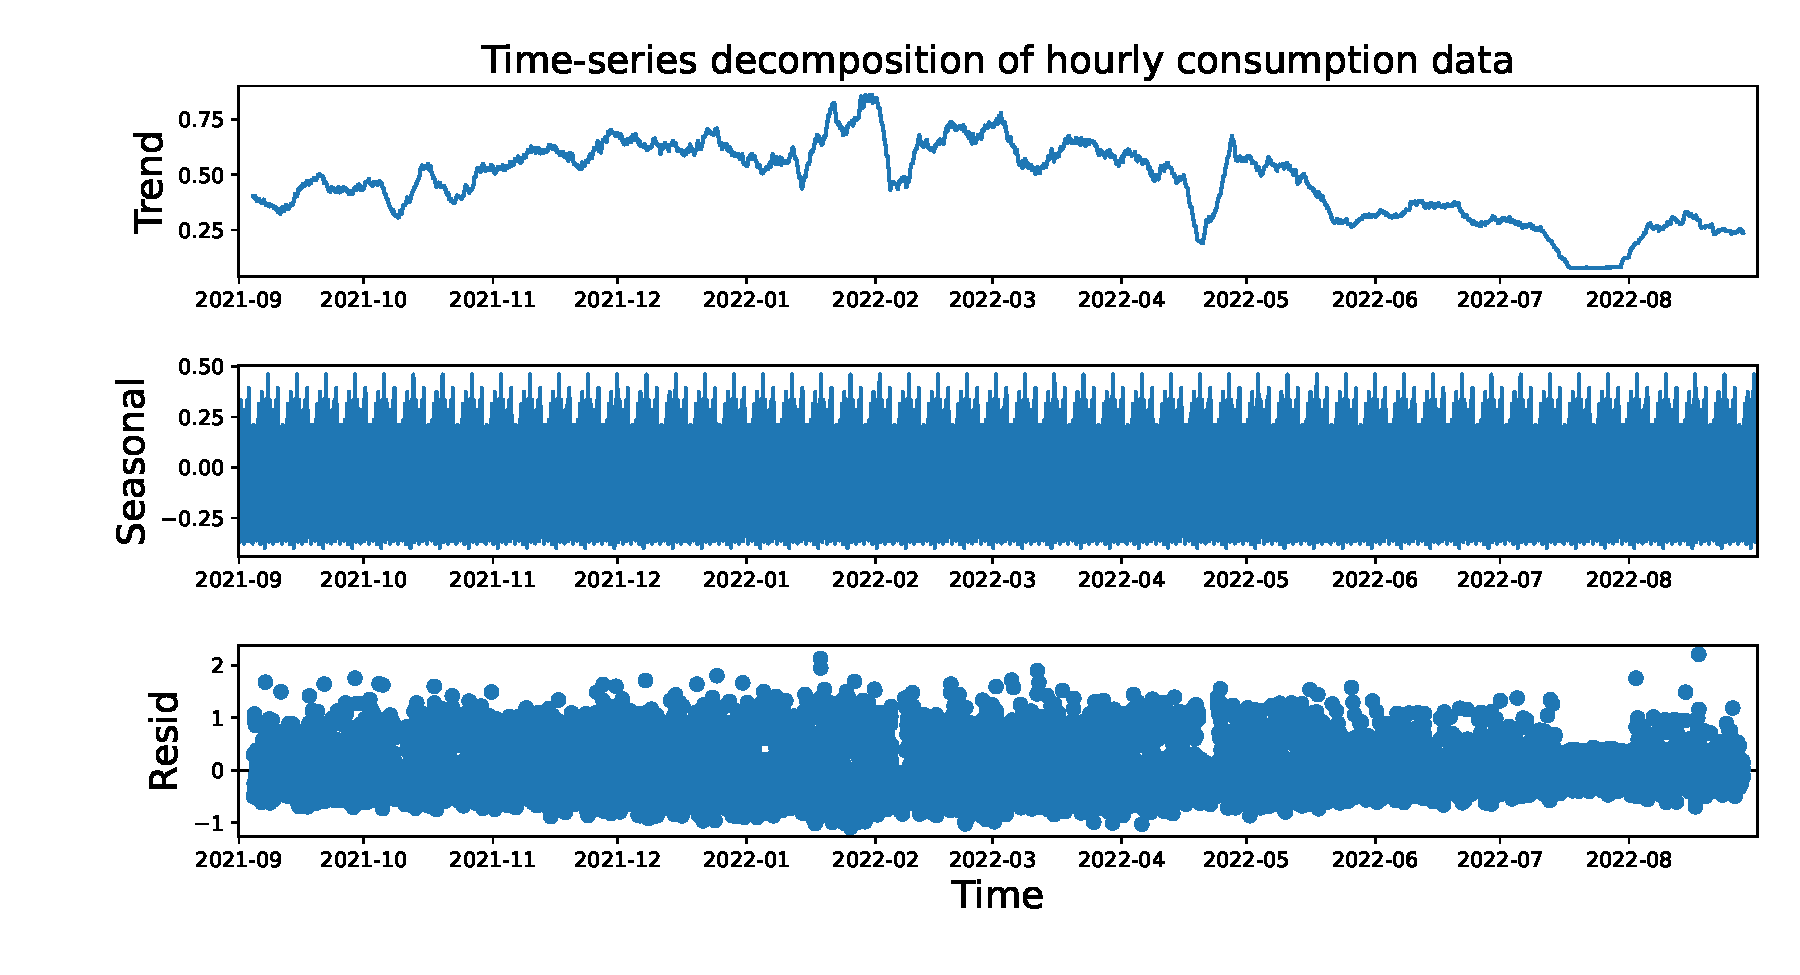
\includegraphics[width=0.5\textwidth]{images/baseline/hourly_decomposition_week_period_customer3}
\subcaption{Third customer.}
\label{fig:decompositioncustomer3}
\end{minipage}
\caption{The time series decompositions of the hourly consumption of the three customers considering as period of the time series a week.}
\end{figure}

\begin{figure}[H]
\begin{minipage}[b]{8.5cm}
\centering
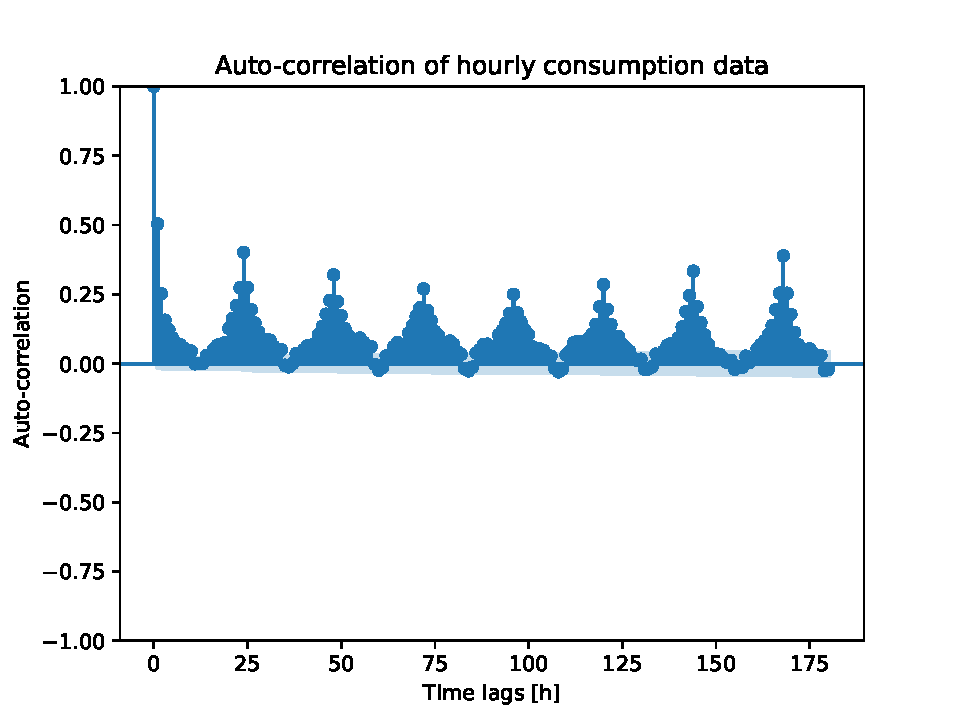
\includegraphics[width=0.8\textwidth]{images/baseline/hourly_correlation_week_range_customer1}
\subcaption{First customer.}
\label{fig:correlationcustomer1}
\end{minipage}
\ \hspace{2mm} \
\begin{minipage}[b]{8.5cm}
\centering
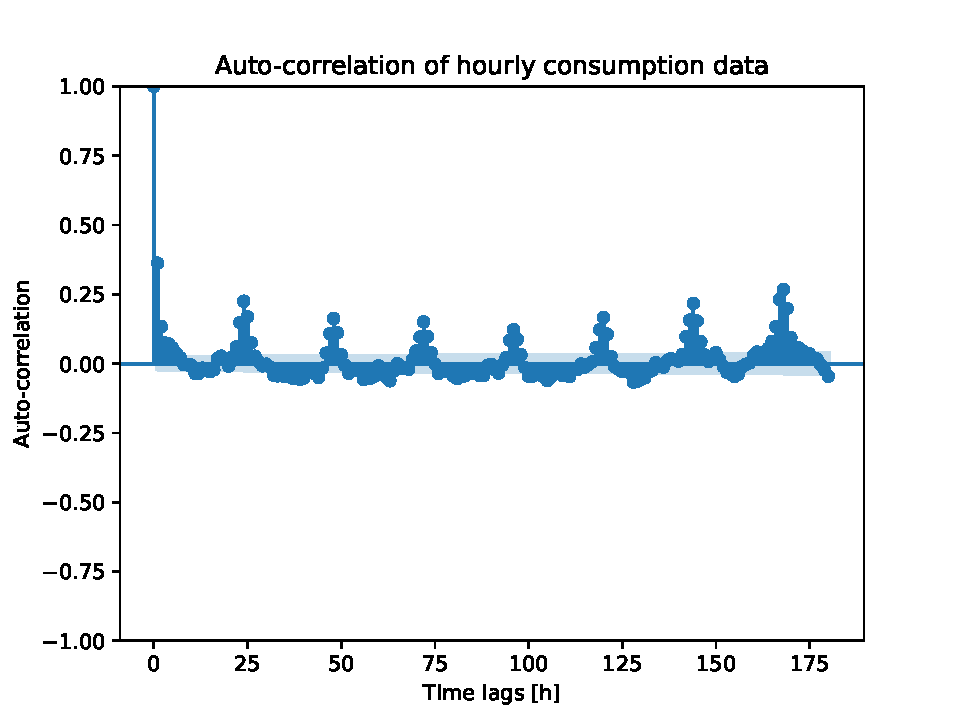
\includegraphics[width=0.8\textwidth]{images/baseline/hourly_correlation_week_range_customer2}
\subcaption{Second customer.}
\label{fig:correlationcustomer2}
\end{minipage}
\begin{minipage}[b]{17cm}
\centering
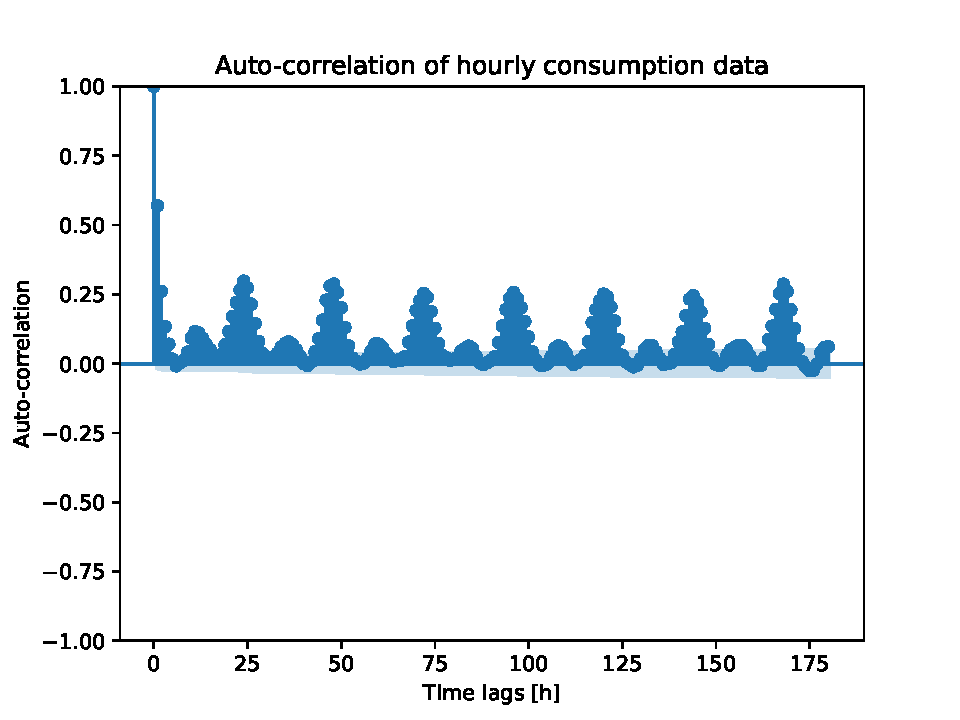
\includegraphics[width=0.4\textwidth]{images/baseline/hourly_correlation_week_range_customer3}
\subcaption{Third customer.}
\label{fig:correlationcustomer3}
\end{minipage}
\caption{The auto-correlations of the hourly consumption of the three customers.}
\end{figure}

\begin{figure}[H]
\begin{minipage}[b]{8.5cm}
\centering
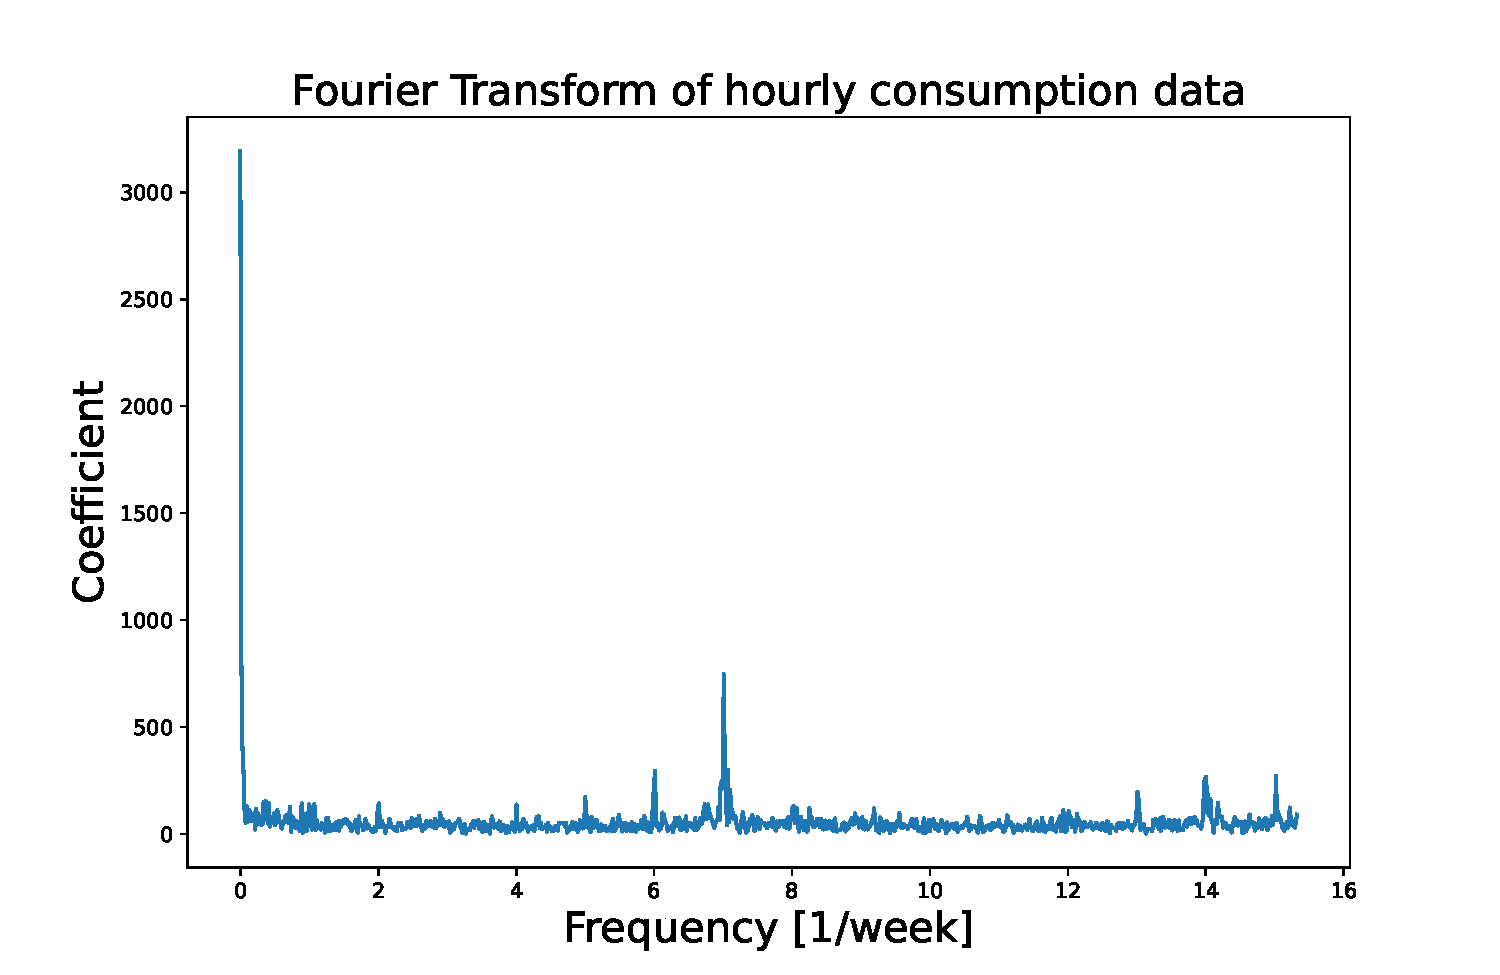
\includegraphics[width=0.8\textwidth]{images/baseline/ft_hour_week_customer1}
\subcaption{First customer.}
\label{fig:ftcustomer1}
\end{minipage}
\ \hspace{2mm} \
\begin{minipage}[b]{8.5cm}
\centering
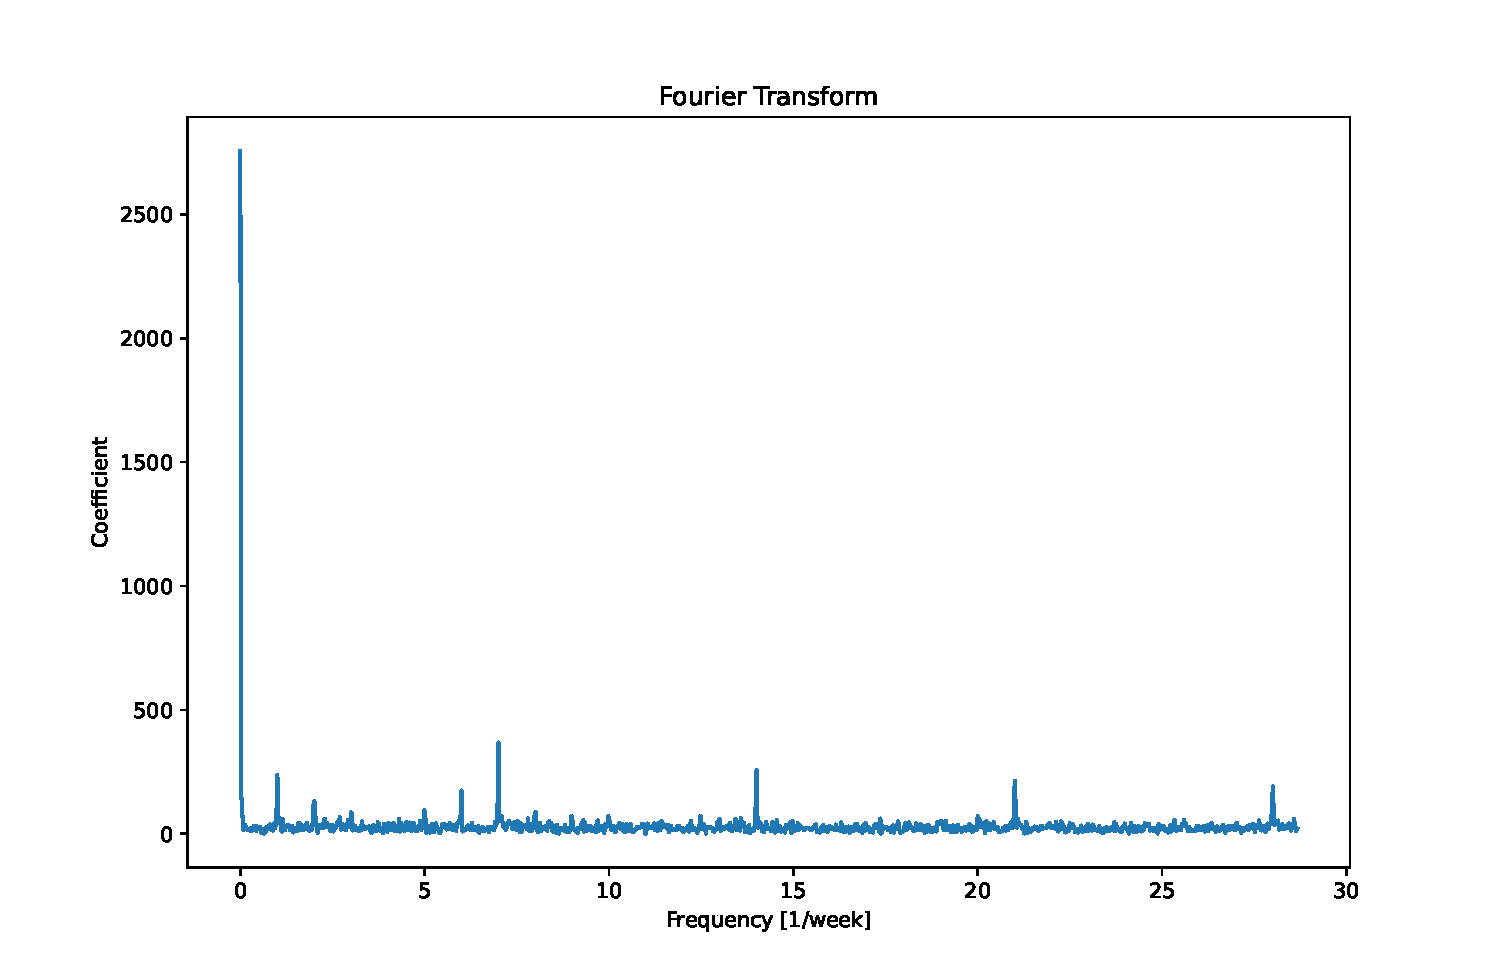
\includegraphics[width=0.8\textwidth]{images/baseline/ft_hour_week_customer2}
\subcaption{Second customer.}
\label{fig:ftcustomer2}
\end{minipage}
\begin{minipage}[b]{17cm}
\centering
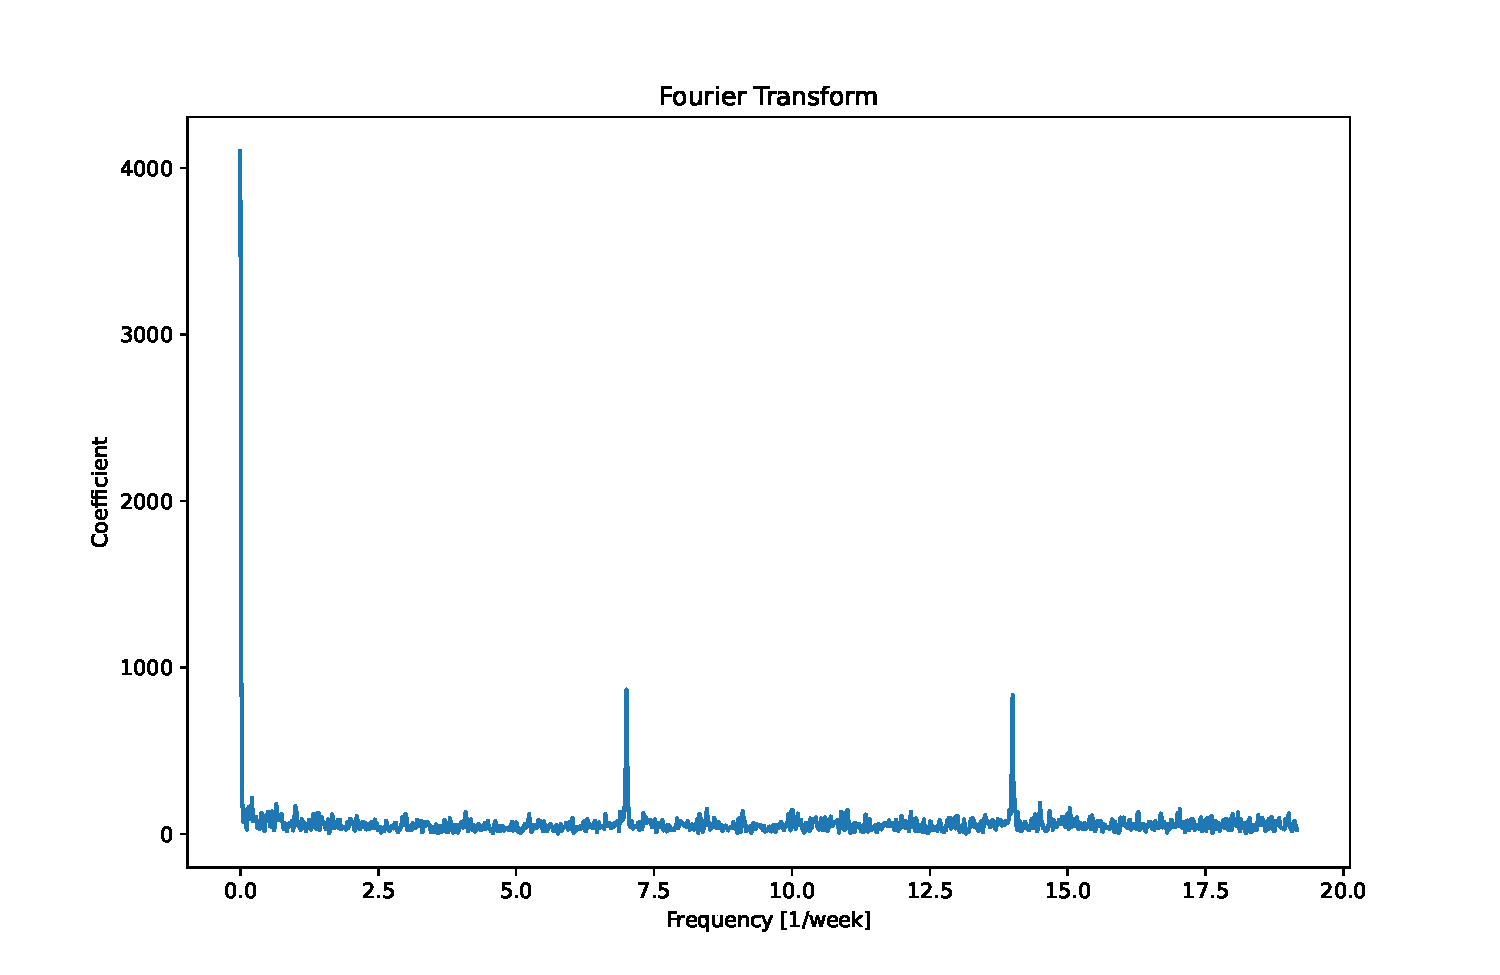
\includegraphics[width=0.4\textwidth]{images/baseline/ft_hour_week_customer3}
\subcaption{Third customer.}
\label{fig:ftcustomer3}
\end{minipage}
\caption{The coefficients given by the Fourier transform of the hourly consumption of the three customers.}
\end{figure}

The auto-correlations of the hourly consumption of the three customers are reported in figure~\ref{fig:correlationcustomer1}, figure~\ref{fig:correlationcustomer2}, and figure~\ref{fig:correlationcustomer3}.
All the customers’ consumptions are not very auto-correlated, it can be shown that the maximum auto-correlation value is around 0.5 in the closest time lag and that there is a peak every 24 hours, with a slightly greater value at one week distance.
This indicates that the consumption data from the closest time lag, as well as those corresponding to the same hour in the preceding days and even better in the preceding weeks, may be valuable features for predicting a time instant's demand.
A reasonable balance can be achieved by incorporating the consumption data from the past 14 days.

The coefficients given by the Fourier transform for the hourly consumption of the three customers are reported in figure~\ref{fig:ftcustomer1}, figure~\ref{fig:ftcustomer2}, and figure~\ref{fig:ftcustomer3}.
The graphical representations show for all the customers a main frequency at the daily periodicity.
Other minor peaks are present mostly at multiples of the 1/day frequency, in particular for the third customer where the 2/day frequency is almost equal to the 1/day.

The daily consumption of the three customers are reported in figure~\ref{fig:dataplotdaycustomer1}, figure~\ref{fig:dataplotdaycustomer2}, and figure~\ref{fig:dataplotdaycustomer3}.

\begin{figure}[H]
\begin{minipage}[b]{8.5cm}
\centering
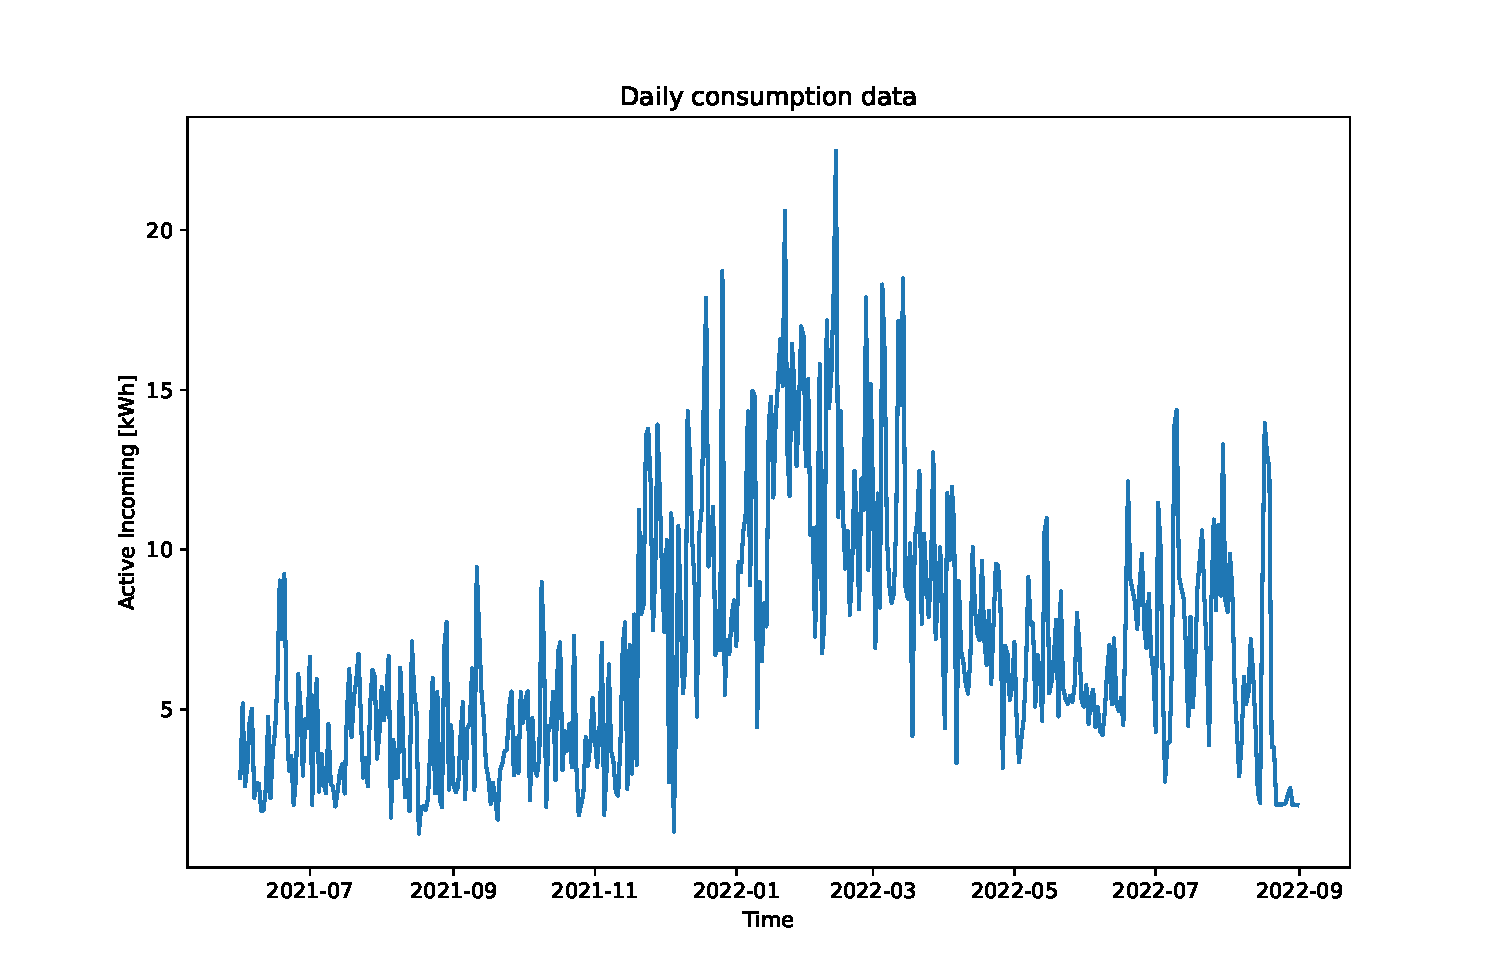
\includegraphics[width=1\textwidth]{images/baseline/data_day_aggregated_plot_customer1}
\subcaption{First customer.}
\label{fig:dataplotdaycustomer1}
\end{minipage}
\ \hspace{2mm} \
\begin{minipage}[b]{8.5cm}
\centering
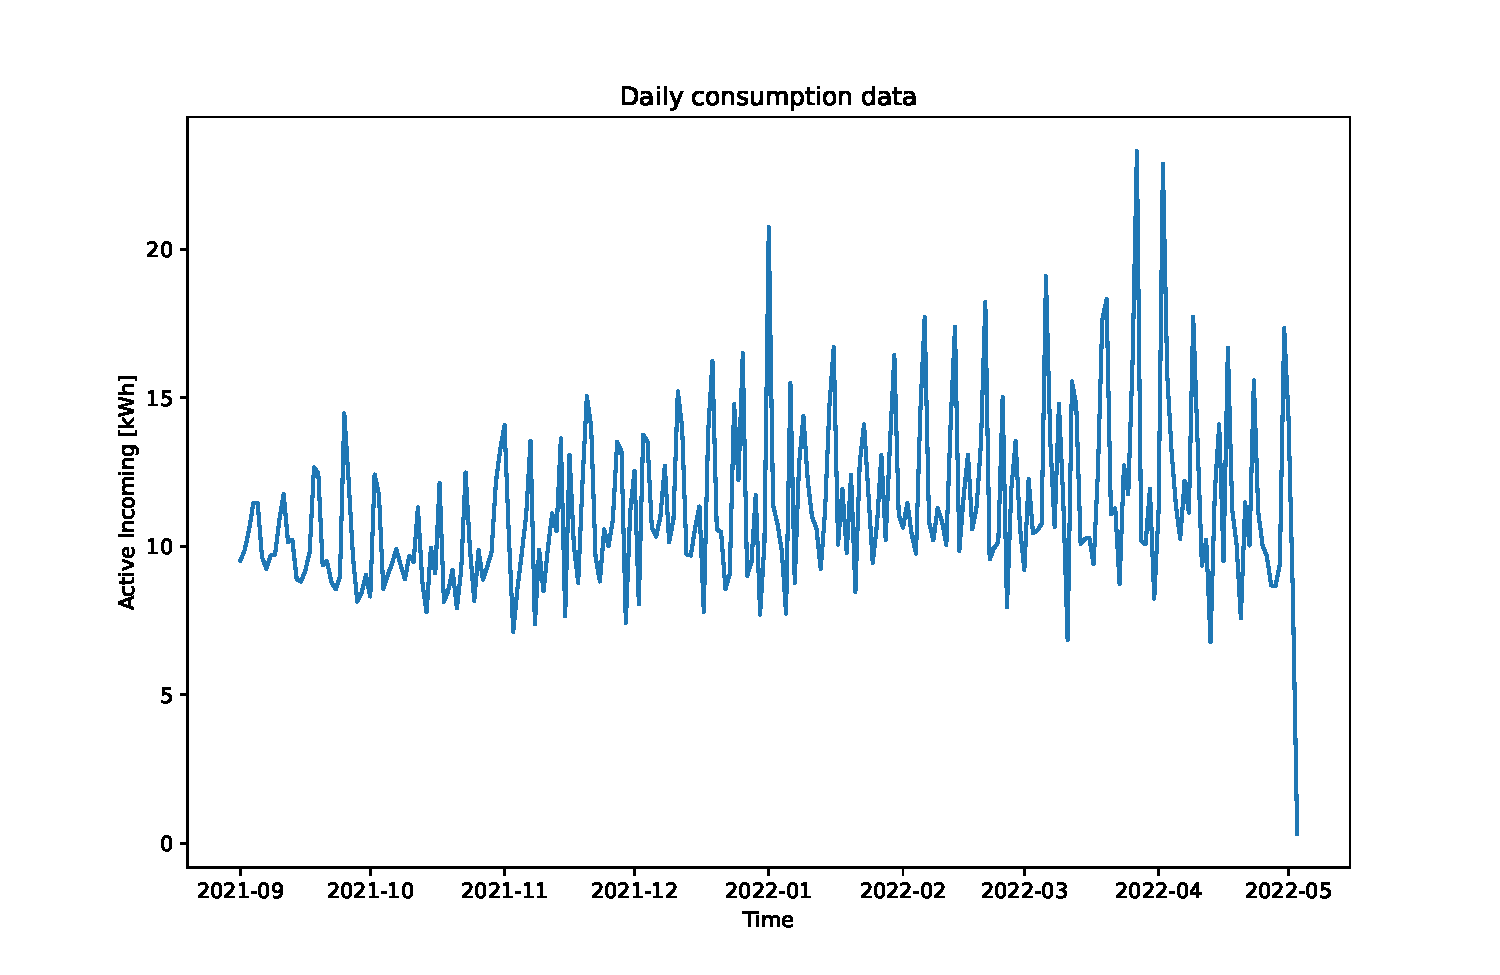
\includegraphics[width=1\textwidth]{images/baseline/data_day_aggregated_plot_customer2}
\subcaption{Second customer.}
\label{fig:dataplotdaycustomer2}
\end{minipage}
\begin{minipage}[b]{17cm}
\centering
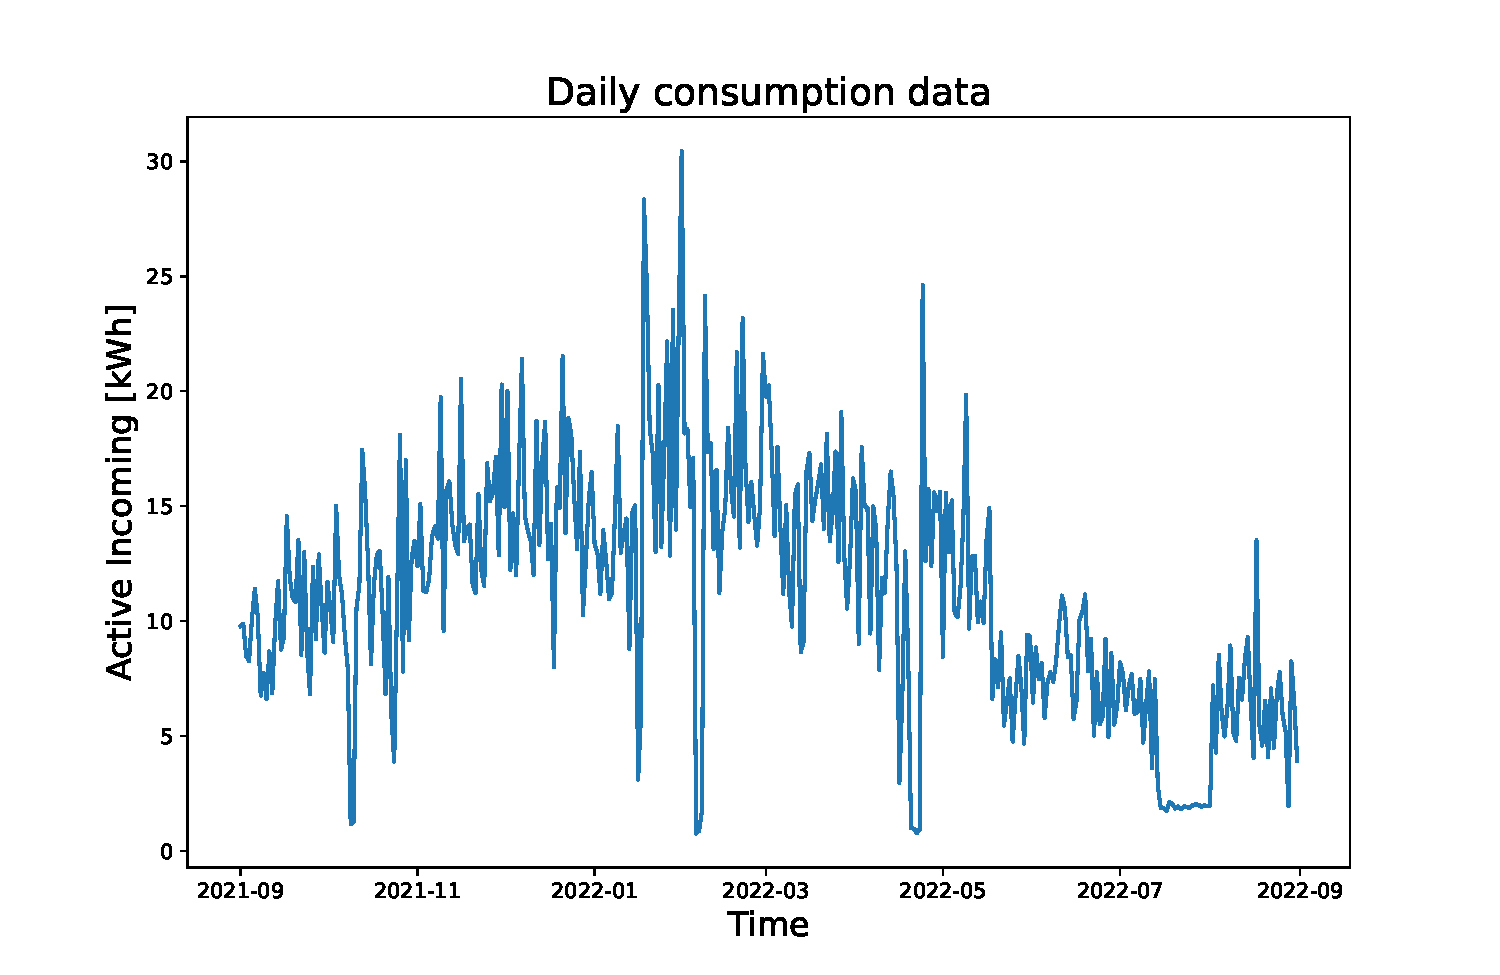
\includegraphics[width=0.5\textwidth]{images/baseline/data_day_aggregated_plot_customer3}
\subcaption{Third customer.}
\label{fig:dataplotdaycustomer3}
\end{minipage}
\caption{The daily consumption of the three customers.}
\end{figure}

The time series decompositions using an additive model of the daily consumption of the three customers considering as period of the time series a week are reported in figure~\ref{fig:decompositiondaycustomer1}, figure~\ref{fig:decompositiondaycustomer2}, and figure~\ref{fig:decompositiondaycustomer3}.
The decomposition is consistent with the hourly aggregated consumption over the customers.

The auto-correlations of the daily consumption of the three customers are reported in figure~\ref{fig:correlationdaycustomer1},  figure~\ref{fig:correlationdaycustomer2}, and  figure~\ref{fig:correlationdaycustomer3}.
With the daily granularity, all the customers’ consumptions show a slightly high value with respect to the hourly granularity.
It can be shown that for the first and third customers, the auto-correlation value is slightly high in the closest time lag and then decreases with the days, with a slightly greater value at one week distance.
Instead, for the second customer the only relevant values are only at a multiple of 7 days.

The coefficients given by the Fourier transform for the daily consumption of the three customers are reported in figure~\ref{fig:ftdaycustomer1}, figure~\ref{fig:ftdaycustomer2}, and figure~\ref{fig:ftdaycustomer3}.
The graphical representation exhibits that there are no main frequencies in the daily consumption of the first and third customers.
Instead, for the second customer there is a small peak at the daily periodicity.

As can be noticed from the data, there is high variability in consumption and low auto-correlation, this suggests how it is difficult to produce highly accurate results on a single customer level.
With just the time series of a few users, it is very difficult to learn a well-performing model, having more users it could be possible to learn certain generic trends or standard behaviors.

Basic data is enhanced with the air temperature, the apparent temperature, and the relative humidity since they are considered the only weather features capable of influencing customers' energy consumption.
To assess the relationship between these weather variables and the consumption of the three customers, two correlation coefficients were used: Pearson's correlation coefficient and Spearman's rank correlation coefficient.
Pearson's correlation coefficient measures the strength of the linear relationship between two variables, while Spearman's rank correlation coefficient measures the strength of the monotonic relationship.
The pearsonr and spearmanr methods of the SciPy library were used to compute the correlation with weather data.

\begin{figure}[H]
\begin{minipage}[b]{8.5cm}
\centering
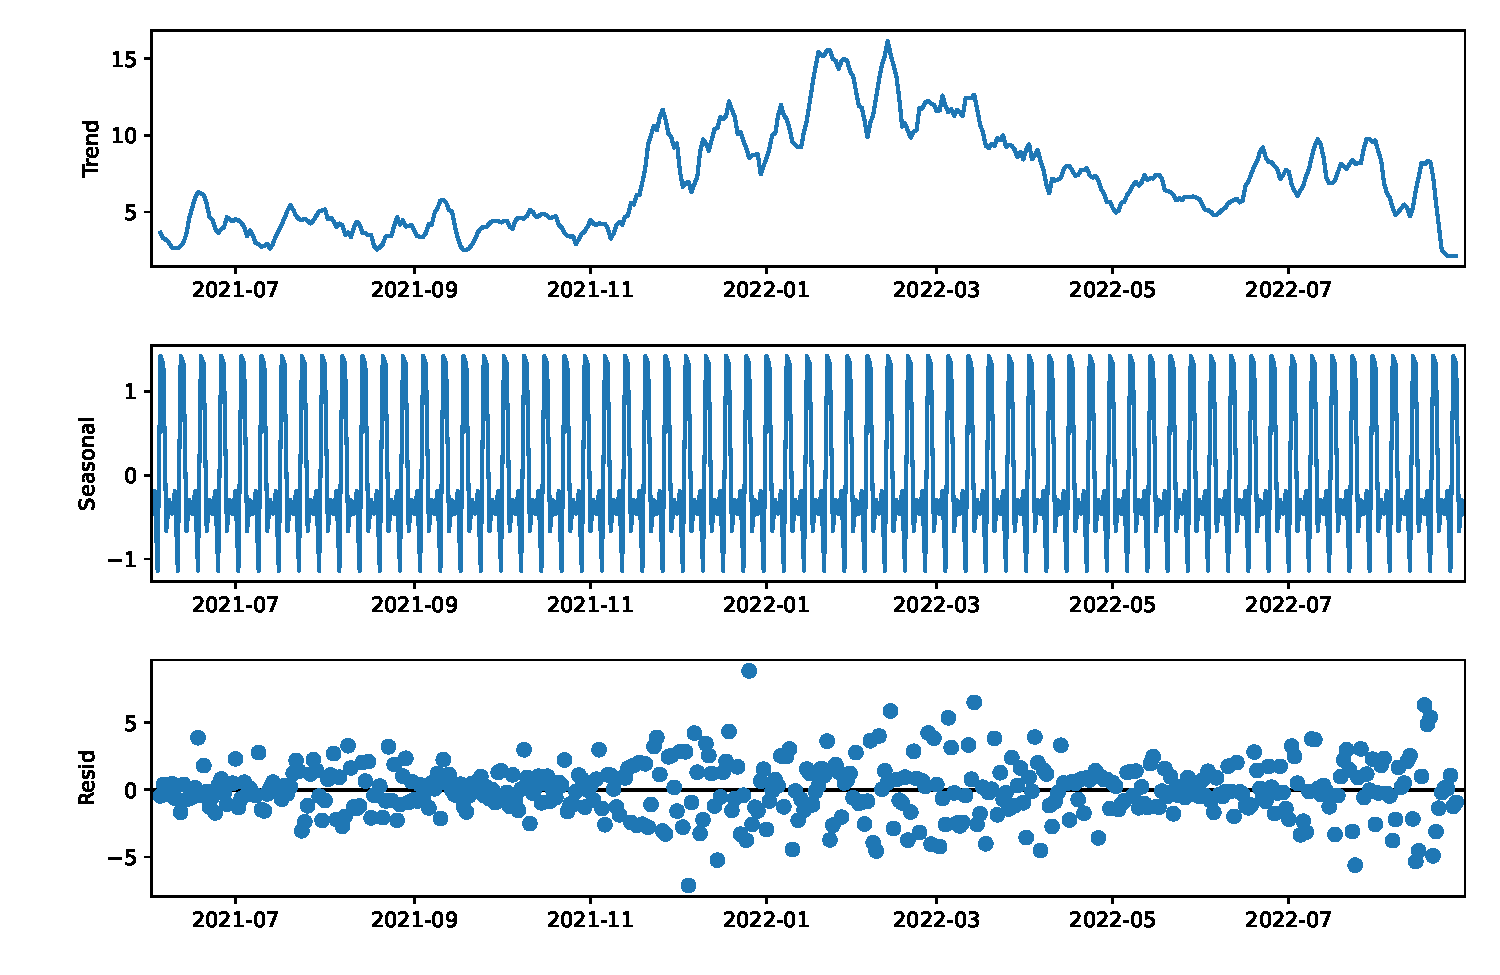
\includegraphics[width=1\textwidth]{images/baseline/daily_aggregated_decomposition_customer1}
\subcaption{First customer.}
\label{fig:decompositiondaycustomer1}
\end{minipage}
\ \hspace{2mm} \
\begin{minipage}[b]{8.5cm}
\centering
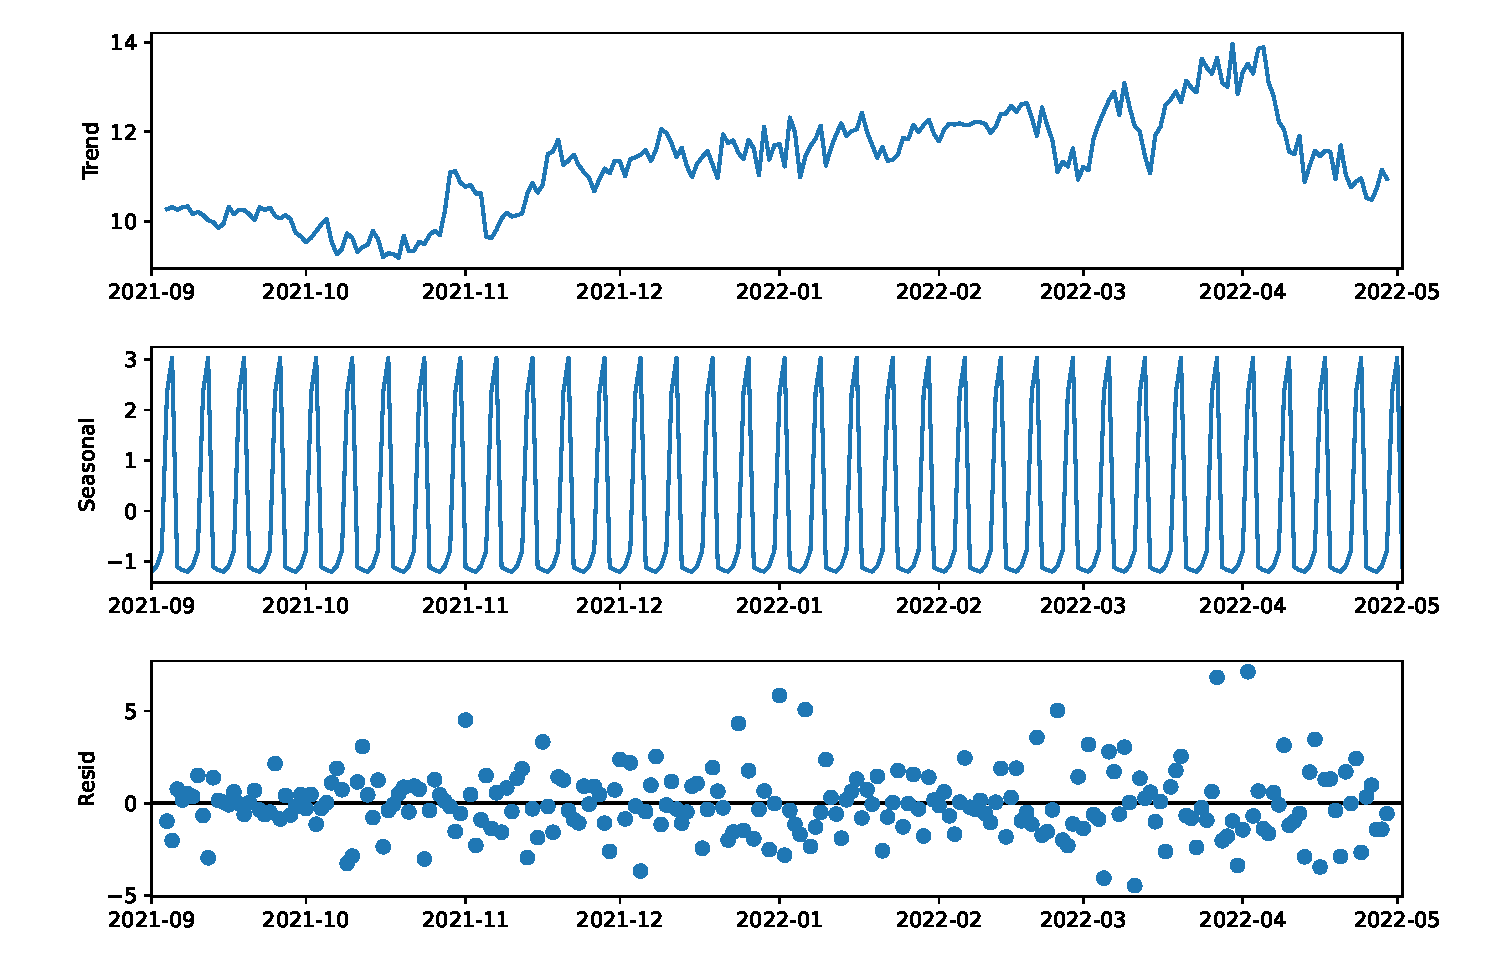
\includegraphics[width=1\textwidth]{images/baseline/daily_aggregated_decomposition_customer2}
\subcaption{Second customer.}
\label{fig:decompositiondaycustomer2}
\end{minipage}
\begin{minipage}[b]{17cm}
\centering
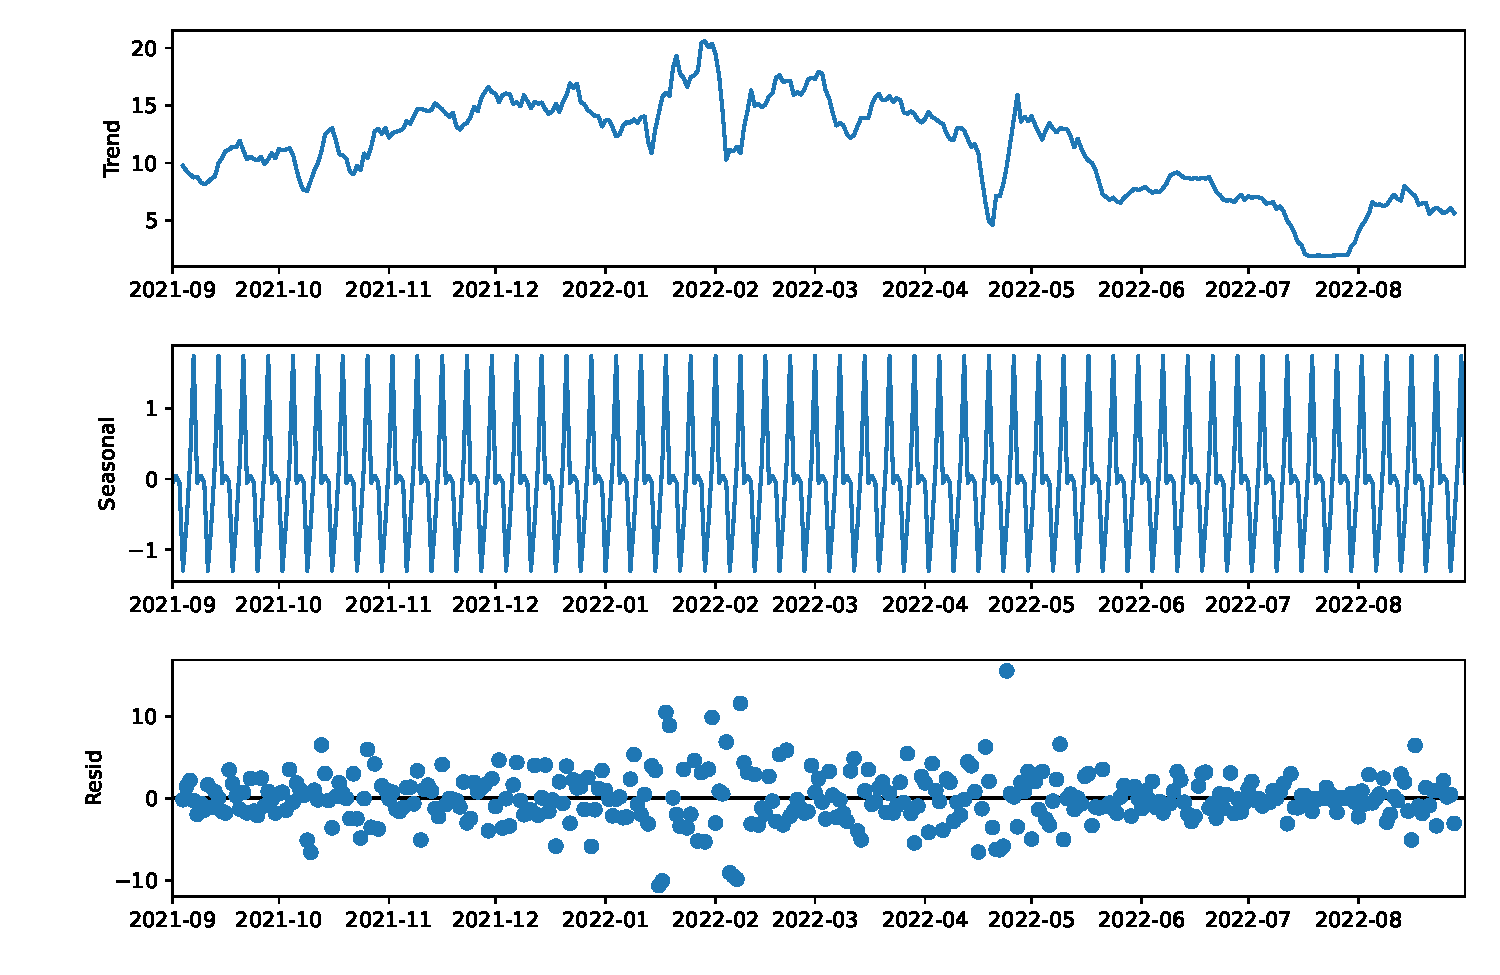
\includegraphics[width=0.5\textwidth]{images/baseline/daily_aggregated_decomposition_customer3}
\subcaption{Third customer.}
\label{fig:decompositiondaycustomer3}
\end{minipage}
\label{fig:decompositiondaycustomer}
\caption{The time series decompositions of the daily consumption of the three customers considering as period of the time series a week.}
\end{figure}

\begin{figure}[H]
\begin{minipage}[b]{8.5cm}
\centering
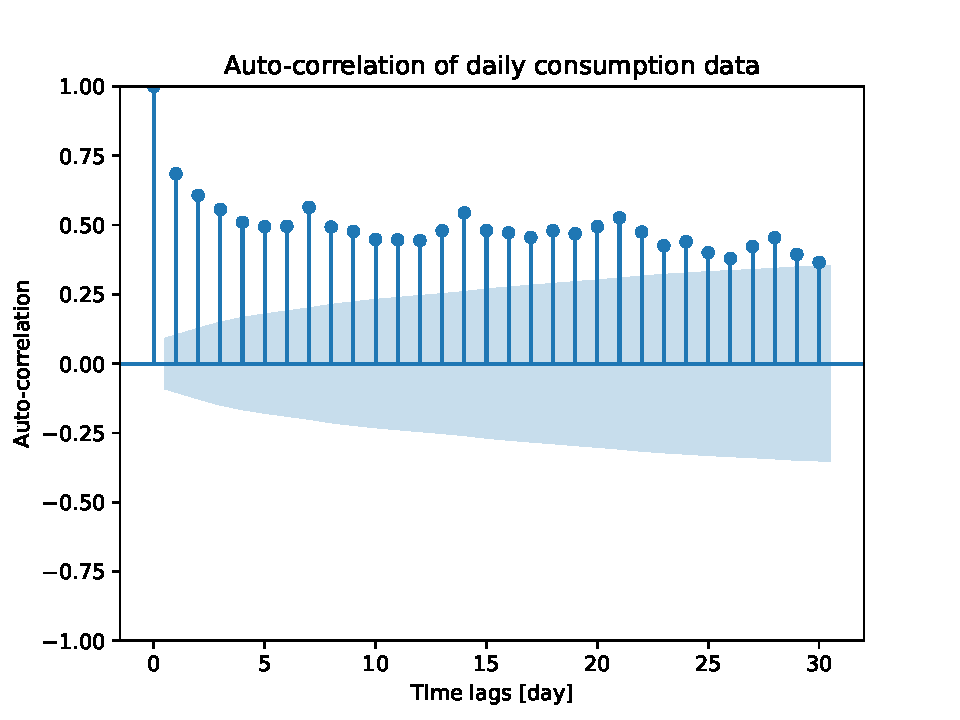
\includegraphics[width=0.8\textwidth]{images/baseline/daily_aggregated_correlation_customer1}
\subcaption{First customer.}
\label{fig:correlationdaycustomer1}
\end{minipage}
\ \hspace{2mm} \
\begin{minipage}[b]{8.5cm}
\centering
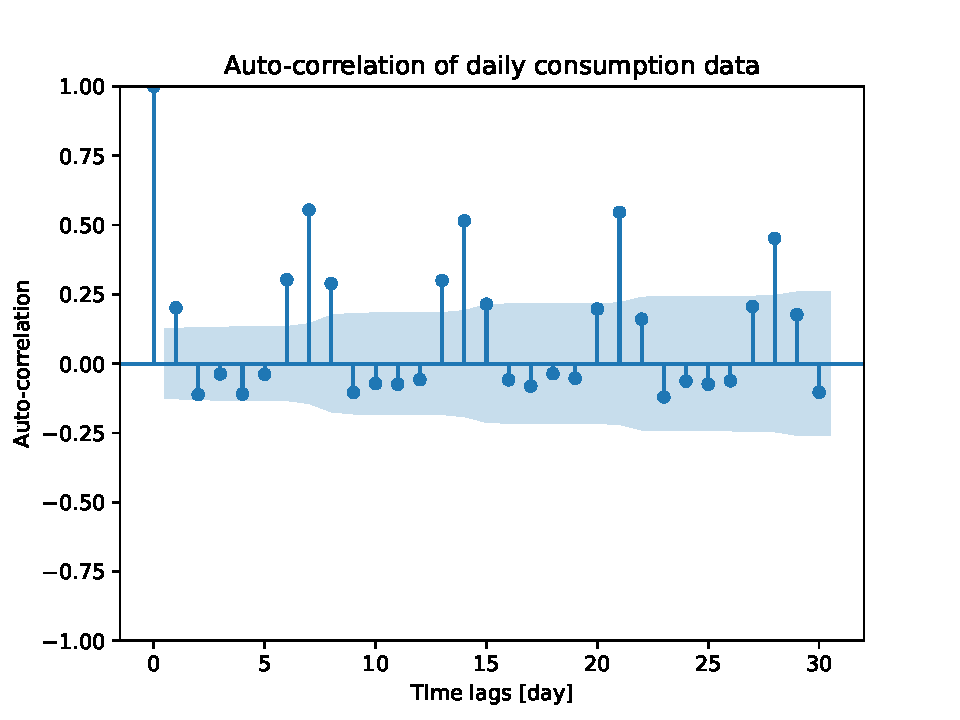
\includegraphics[width=0.8\textwidth]{images/baseline/daily_aggregated_correlation_customer2}
\subcaption{Second customer.}
\label{fig:correlationdaycustomer2}
\end{minipage}
\begin{minipage}[b]{17cm}
\centering
\includegraphics[width=0.4\textwidth]{images/baseline/daily_aggregated_correlation_customer3}
\subcaption{Third customer.}
\label{fig:correlationdaycustomer3}
\end{minipage}
\caption{The auto-correlations of the daily consumption of the three customers.}
\end{figure}

\begin{figure}[H]
\begin{minipage}[b]{8.5cm}
\centering
\includegraphics[width=0.8\textwidth]{images/baseline/ft_day_customer1}
\subcaption{First customer.}
\label{fig:ftdaycustomer1}
\end{minipage}
\ \hspace{2mm} \
\begin{minipage}[b]{8.5cm}
\centering
\includegraphics[width=0.8\textwidth]{images/baseline/ft_day_customer2}
\subcaption{Second customer.}
\label{fig:ftdaycustomer2}
\end{minipage}
\begin{minipage}[b]{17cm}
\centering
\includegraphics[width=0.4\textwidth]{images/baseline/ft_day_customer3}
\subcaption{Third customer.}
\label{fig:ftdaycustomer3}
\end{minipage}
\caption{The coefficients given by the Fourier transform of the daily consumption of the three customers.}
\end{figure}

The results showed that the hourly consumption of the three customers had:
\begin{itemize}
  \item a Pearson correlation coefficient of -0.2491, 0.0240, and -0.1338 respectively and a Spearman's rank correlation coefficient of -0.2088, 0.1304, and -0.0196 respectively with respect to the air temperature;
  \item a Pearson correlation coefficient of -0.2434, 0.0266, and -0.1356 respectively and a Spearman's rank correlation coefficient of -0.2082, 0.1305, and -0.0207 respectively with respect to the apparent temperature;
  \item a Pearson correlation coefficient of 0.1193, -0.0845, and -0.0985 respectively and a Spearman's rank correlation coefficient of 0.1491, -0.1048, and -0.1123 respectively with respect to the relative humidity.
\end{itemize}
It can be noticed that both the coefficients indicate a weak correlation between the weather variables and the consumption of the three customers, nevertheless, it may still be useful to incorporate weather data into the prediction models since also the auto-correlation values are not particularly high.

The results showed that the daily consumption of the three customers had:
\begin{itemize}
  \item a Pearson correlation coefficient of -0.5542, -0.2341, and -0.6727 respectively and a Spearman's rank correlation coefficient of -0.5164, -0.2592, and -0.6978 respectively with respect to the air temperature;
  \item a Pearson correlation coefficient of -0.5361, -0.2329, and -0.6787 respectively and a Spearman's rank correlation coefficient of -0.5166, -0.2584, and -0.7004 respectively with respect to the apparent temperature;
  \item a Pearson correlation coefficient of 0.1264, 0.0199, and 0.1407 respectively and a Spearman's rank correlation coefficient of 0.1412, 0.0506, and 0.2104 respectively with respect to the relative humidity.
\end{itemize}
It can be noticed that both the coefficients increased considering the daily data meaning that the mean weather data over the day is more correlated to the daily consumption of the three considered customers, compared to the hourly granularity.

As described in chapter~\ref{cha:implementation}, tariff granularity has also been thought of as a possible granularity.
Tariff granularity assumes that the tariff is a control signal capable of modifying consumption.
However, after some initial experimental results with this granularity showing unsatisfactory performance, this granularity was not further investigated.
Though, this granularity can be investigated in a possible future work to understand whether it could be applicable to produce good results.

After this data analysis, the specific parameters used in the models can be explained more in detail.
The parameters for the different models were tested and verified on training data to result in the best-performing models, this was done by trying different values and configurations.
The baseline approaches are built considering the repetition of past days and weeks since data presents a high correlation with that time instants and could lead to a reasonable baseline performance to achieve.
Instead of just considering the one-day and one-week baselines, for this use case also the four-week and the twelve-week baselines are considered taking an average of the consumption in the specified number of previous weeks.
This is because averaging the consumption over the previous week may lead to a more robust prediction considering a month and a trimester range,
The SARIMA model considers the week as the period for seasonal differencing since data presents a high correlation with that time instants and the model can try to take advantage of the weekly seasonality.
The support vector regressor model uses a radial basis function kernel with a configuration of the C parameter (regularization parameter of squared l2 penalty) to 1.0 to penalize the complexity of the model, and the epsilon parameter defining the epsilon-tube for no penalty to 0.1 as a trade-off between accuracy and generalization.
The hist gradient boosting regressor model uses as loss the absolute error.
The learning rate was set to 0.1, 100 estimators were used and l2 regularization was not set.
The parameters for tree definition are 31 as the maximum number of leaves, depth is not constrained, 20 as the minimum number of samples per leaf, and 255 as the maximum number of bins.
For the extreme gradient boosting regressor model, tree-based models were used and the construction algorithm is automatically chosen by heuristic to choose the fastest method.
It uses a squared loss since this was the supported metric closer to our evaluation metric.
The learning rate was set to 0.3, 100 estimators were used and l2 regularization was set with a weight of 1.0.
The parameters for tree definition are 6 as the maximum depth, and the maximum number of leaves is not constrained.
The Prophet model was built keeping the default parameters for automatically detecting seasonalities and best fitting the training data.

The LSTM model was designed as a 2-layer model with 32 Bidirectional LSTM units in the first layer which use ReLU activation function and sigmoid as recurrent activation function with both dropout and recurrent dropout of 0.02.
The second layer is composed of 16 Bidirectional LSTM units which use ReLU activation function and sigmoid as recurrent activation function without dropout and recurrent dropout.
The output of the layer goes inside a dense unit to output the final prediction.
The model is trained using a combination of mean absolute error and mean absolute percentage error as loss and Nadam as optimizer with a learning rate of 0.005.

The GRU model was designed as a 2-layer model with 32 Bidirectional GRU units in the first layer which use ReLU activation function and sigmoid as recurrent activation function with both dropout and recurrent dropout of 0.02.
Subsequently, the second layer is composed of 16 Bidirectional GRU units which use ReLU activation function and sigmoid as recurrent activation function without dropout and recurrent dropout.
The output of the layer goes inside a dense unit to output the final prediction.
The model is trained using a combination of mean absolute error and mean absolute percentage error as loss and Nadam as optimizer with a learning rate of 0.005.

The CNN model was designed as a 2-layer model with a first layer composed of 32 1D Convolutional units with a kernel size of 5 which uses ReLU activation function.
A 1D max polling operation is applied before entering the second layer composed of 16 1D Convolutional units with a kernel size of 3 which use ReLU activation function.
A 1D max polling operation is applied before the flattening operation and entering the final dense unit to output the final prediction.
The model is trained using a combination of mean absolute error and mean absolute percentage error as loss and Nadam as optimizer with a learning rate of 0.005.

The TFT model was configured with 2 LSTM layers with 16 as hidden size, 4 as attention size, and 8 as hidden continuous size.
The dropout is set to 0.02.
The model is trained using mean absolute percentage error as loss and Nadam as optimizer with a learning rate of 0.005.

% first customer
% \begin{table}[H]
% \centering
% \begin{tabular}{|c|c|c|}
% \hline
%  & \textbf{Blocked k-fold} & \textbf{Test on the last split}\\
% \textbf{Model} & \textbf{cross-validation} & \textbf{MAPE | MAE [kWh]}\\
%  & \textbf{MAPE | MAE [kWh]} & \\
% \hline
% HistGradientBoostingRegressor & 62.05 $\pm$ 15.29 | 0.132 $\pm$ 0.046 & 27.60 | 0.021\\
% \hline
% One Day Baseline & 171.37 $\pm$ 148.43 | 0.209 $\pm$ 0.083 & 48.44 | 0.028\\
% \hline
% GRU & 54.80 $\pm$ 8.11 | 0.235 $\pm$ 0.067 & 33.50 | 0.049\\
% \hline
% LSTM & 133.17 $\pm$ 207.08 | 0.294 $\pm$ 0.145 & 33.69 | 0.049\\
% \hline
% TFT & 74.25 $\pm$ 34.86 | 0.219 $\pm$ 0.066 & 39.10 | 0.055\\
% \hline
% XGBRegressor & 117.86 $\pm$ 31.29 | 0.157 $\pm$ 0.038 & 120.87 | 0.067\\
% \hline
% CNN & 167.29 $\pm$ 49.74 | 0.303 $\pm$ 0.067 & 165.55 | 0.110\\
% \hline
% SVR & 108.71 $\pm$ 33.24 | 0.225 $\pm$ 0.056 & 201.16 | 0.121\\
% \hline
% One Week Baseline & 178.58 $\pm$ 76.74 | 0.226 $\pm$ 0.039 & 322.74 | 0.166\\
% \hline
% 4 Week Baseline & 196.68 $\pm$ 78.00 | 0.228 $\pm$ 0.034 & 379.96 | 0.194\\
% \hline
% 12 Week Baseline & 225.54 $\pm$ 86.94 | 0.260 $\pm$ 0.029 & 453.56 | 0.231\\
% \hline
% SARIMA & 278.71 $\pm$ 63.55 | 0.325 $\pm$ 0.059 & 513.50 | 0.252\\
% \hline
% Prophet & 215.51 $\pm$ 113.13 | 0.253 $\pm$ 0.025 & 487.29 | 0.258\\
% \hline
% \end{tabular}
% \caption{Table summarizing the results for hourly granularity.}
% \label{tab:baselinehourlyresults}
% \end{table}

% second customer
\begin{table}[H]
\centering
\begin{tabular}{|c|c|c|}
\hline
 & \textbf{Blocked k-fold} & \textbf{Test on the last split}\\
\textbf{Model} & \textbf{cross-validation} & \textbf{MAPE | MAE [kWh]}\\
 & \textbf{MAPE | MAE [kWh]} & \\
\hline
TFT & 47.33 $\pm$ 5.57 | 0.287 $\pm$ 0.028 & 44.19 | 0.231\\
\hline
HistGradientBoostingRegressor & 53.95 $\pm$ 7.02 | 0.260 $\pm$ 0.023 & 50.41 | 0.231\\
\hline
SVR & 60.30 $\pm$ 6.81 | 0.278 $\pm$ 0.032 & 60.41 | 0.243\\
\hline
SARIMA & 74.17 $\pm$ 10.01 | 0.271 $\pm$ 0.021 & 78.02 | 0.244\\
\hline
XGBRegressor & 73.71 $\pm$ 9.54 | 0.275 $\pm$ 0.024 & 68.07 | 0.245\\
\hline
Prophet & 83.84 $\pm$ 10.23 | 0.280 $\pm$ 0.020 & 81.92 | 0.249\\
\hline
GRU & 58.88 $\pm$ 19.55 | 0.309 $\pm$ 0.041 & 42.55 | 0.257\\
\hline
LSTM & 111.87 $\pm$ 212.07 | 0.464 $\pm$ 0.516 & 44.23 | 0.266\\
\hline
4 Week Baseline & 74.06 $\pm$ 12.51 | 0.275 $\pm$ 0.027 & 79.07 | 0.266\\
\hline
12 Week Baseline & 74.30 $\pm$ 13.66 | 0.266 $\pm$ 0.024 & 89.23 | 0.278\\
\hline
One Week Baseline & 82.69 $\pm$ 12.83 | 0.326 $\pm$ 0.030 & 70.48 | 0.281\\
\hline
One Day Baseline & 75.80 $\pm$ 13.96 | 0.318 $\pm$ 0.035 & 71.25 | 0.292\\
\hline
CNN & 148.16 $\pm$ 30.05 | 0.510 $\pm$ 0.105 & 70.19 | 0.318\\
\hline
\end{tabular}
\caption{Table summarizing the results for hourly granularity.}
\label{tab:baselinehourlyresults}
\end{table}

% third customer
% \begin{table}[H]
% \centering
% \begin{tabular}{|c|c|c|}
% \hline
%  & \textbf{Blocked k-fold} & \textbf{Test on the last split}\\
% \textbf{Model} & \textbf{cross-validation} & \textbf{MAPE | MAE [kWh]}\\
%  & \textbf{MAPE | MAE [kWh]} & \\
% \hline
% HistGradientBoostingRegressor & 62.36 $\pm$ 26.63 | 0.142 $\pm$ 0.071 & 54.29 | 0.119\\
% \hline
% SVR & 146.78 $\pm$ 53.02 | 0.205 $\pm$ 0.043 & 92.01 | 0.160\\
% \hline
% XGBRegressor & 121.36 $\pm$ 34.22 | 0.184 $\pm$ 0.068 & 103.16 | 0.161\\
% \hline
% 12 Week Baseline & 214.61 $\pm$ 94.84 | 0.256 $\pm$ 0.046 & 122.51 | 0.175\\
% \hline
% SARIMA & 170.81 $\pm$ 67.39 | 0.223 $\pm$ 0.051 & 124.07 | 0.176\\
% \hline
% 4 Week Baseline & 151.74 $\pm$ 67.48 | 0.218 $\pm$ 0.046 & 110.45 | 0.180\\
% \hline
% One Week Baseline & 142.69 $\pm$ 69.22 | 0.232 $\pm$ 0.094 & 102.25 | 0.190\\
% \hline
% Prophet & 200.64 $\pm$ 59.18 | 0.255 $\pm$ 0.031 & 147.07 | 0.208\\
% \hline
% LSTM & 101.84 $\pm$ 4.67 | 0.246 $\pm$ 0.095 & 97.98 | 0.233\\  % TODO relaunch
% \hline
% GRU & 99.92 $\pm$ 5.13 | 0.243 $\pm$ 0.093 & 99.31 | 0.235\\  % TODO relaunch
% \hline
% TFT & 100.22 $\pm$ 44.40 | 0.242 $\pm$ 0.109 & 105.18 | 0.243\\
% \hline
% One Day Baseline & 151.22 $\pm$ 89.08 | 0.242 $\pm$ 0.101 & 162.76 | 0.247\\
% \hline
% CNN & 1749.85 $\pm$ 2806.48 | 2.035 $\pm$ 3.380 & 546.16 | 0.665\\  % TODO relaunch
% \hline
% \end{tabular}
% \caption{Table summarizing the results for hourly granularity.}
% \label{tab:baselinehourlyresults}
% \end{table}

12 splits were used for block validation with a test size of a week each time, namely 7 days of data.
For the hourly granularity, the models start with the total number of entries for the customer minus 2016 entries as training and predict every time 168 entries until reaching the last prediction instant where the model has a training size of the total number of entries for the customer minus the last 168 entries.
The results for hourly granularity for the second customer are reported in table~\ref{tab:baselinehourlyresults}.
Entries are sorted by best MAE using the last split as the test set.
Only this customer is reported since it presents the best results and the models were optimized for this customer.
The blocked k-fold cross-validation suggests that the TFT model has the best MAPE and this is not confirmed on the last split just because there is GRU that performs slightly better in terms of MAPE.
The not-encouraging thing is that even if it is the best model in terms of MAPE, this value is still close to 50\% indicating that on average the predictions are distant from the actual value by half of this value.
TFT is also the best approach in terms of MAE on the last split, but not on the basis of the blocked k-fold cross-validation which indicates that the best model is the hist gradient boosting regressor model.
In general, this data is not well predictable and also the different baselines confirm that having a look at the close history there is no relevant daily or weekly repetition with MAPE and MAE both higher than TFT and hist gradient boosting regressor model.

The AutoML approach uses the mean MAPE forecasting as loss and it is launched for 10 hours with a maximum function evaluation time of 2 hours.
Then the best ensemble of the found models is returned and can be used to forecast.
This approach obtained a one-week MAPE of 61.64\% and a MAE of 0.338 kWh.
In this case, AutoML is not able to achieve very good results compared to many other models but this is probably related to the quality of the data.
It still has great potential as demonstrated in demand prediction and potentially providing more total training time and more data, potentially also of different customers, it can be able to reach better performance.

The forecasts produced by the TFT model for the last split in comparison to the actual values are reported in figure~\ref{fig:baselinetfthourlyforecasts}.
It can be noticed that it is not able to accurately follow the signal since this is very varying from hour to hour.
Although, it is able to somehow predict that there is a peak during the day but it is not able to reach the correct quantity.

\begin{figure}[H]
\centering
\includegraphics[width=1\textwidth]{images/baseline/TFT}
\caption{The forecasts produced by the temporal fusion transoformer model for the last split in comparison to the actual values.}
\label{fig:baselinetfthourlyforecasts}
\end{figure}

The absolute error of forecasts produced by the TFT model for the last split in comparison to the actual values is reported in figure~\ref{fig:baselinetfthourlyforecastsmae}.
While the absolute percentage error of forecasts produced by the TFT model for the last split in comparison to the actual values is reported in figure~\ref{fig:baselinetfthourlyforecastsmape}.
It can be shown that the entity of the errors is quite high both in terms of absolute error and in terms of absolute percentage error.
Moreover, the error signal seems to have some periodicity that the TFT model is not able to capture, probably due to the high variability of the data.
Finally, the scatter plot representing the error of the forecasts produced by the TFT model for the last split in comparison to the actual values is reported in figure~\ref{fig:baselinetfthourlyforecastsscatterplot}.
This scatter plot demonstrates that there is no bias and can be also noticed that the model is conservative and the positive error is contained while the negative ones are up to six times bigger.
The error can be pretty high also when the predicted values are low.

\begin{figure}[H]
\centering
\includegraphics[width=1\textwidth]{images/baseline/TFT_mae}
\caption{The absolute error of forecasts produced by the temporal fusion transoformer model for the last split in comparison to the actual values.}
\label{fig:baselinetfthourlyforecastsmae}
\end{figure}

\begin{figure}[H]
\centering
\includegraphics[width=1\textwidth]{images/baseline/TFT_mape}
\caption{The absolute percentage error of forecasts produced by the temporal fusion transoformer model for the last split in comparison to the actual values.}
\label{fig:baselinetfthourlyforecastsmape}
\end{figure}

\begin{figure}[H]
\centering
\includegraphics[width=1\textwidth]{images/baseline/TFT_error_scatter_plot_predicted}
\caption{The scatter plot representing the error of the forecasts produced by the temporal fusion transoformer model for the last split in comparison to the actual values.}
\label{fig:baselinetfthourlyforecastsscatterplot}
\end{figure}

% first customer
% \begin{table}[H]
% \centering
% \begin{tabular}{|c|c|c|}
% \hline
%  & \textbf{Blocked k-fold} & \textbf{Test on the last split}\\
% \textbf{Model} & \textbf{cross-validation} & \textbf{MAPE | MAE [kWh]}\\
%  & \textbf{MAPE | MAE [kWh]} & \\
% \hline
% One Day Baseline & 63.23 $\pm$ 84.77 | 2.917 $\pm$ 2.111 & 5.86 | 0.140\\
% \hline
% TFT & 57.49 $\pm$ 53.43 | 2.576 $\pm$ 1.169 & 48.81 | 1.010\\
% \hline
% CNN & 65.10 $\pm$ 37.05 | 4.226 $\pm$ 1.829 & 50.93 | 1.092\\
% \hline
% GRU & 46.34 $\pm$ 16.29 | 3.409 $\pm$ 1.652 & 61.09 | 1.298\\
% \hline
% XGBRegressor & 50.01 $\pm$ 31.96 | 2.597 $\pm$ 0.890 & 89.73 | 1.939\\
% \hline
% HistGradientBoostingRegressor & 45.34 $\pm$ 28.64 | 2.362 $\pm$ 0.682 & 102.34 | 2.115\\
% \hline
% LSTM & 59.81 $\pm$ 20.88 | 3.813 $\pm$ 1.425 & 119.40 | 2.522\\
% \hline
% Prophet & 56.81 $\pm$ 39.79 | 3.058 $\pm$ 1.064 & 159.90 | 3.451\\
% \hline
% One Week Baseline & 66.31 $\pm$ 50.24 | 3.036 $\pm$ 1.057 & 166.09 | 3.461\\
% \hline
% SVR & 57.95 $\pm$ 53.96 | 2.677 $\pm$ 1.056 & 206.13 | 4.366\\
% \hline
% 4 Week Baseline & 65.55 $\pm$ 58.37 | 2.830 $\pm$ 0.991 & 215.05 | 4.491\\
% \hline
% SARIMA & 59.67 $\pm$ 46.79 | 2.668 $\pm$ 1.087 & 225.34 | 4.790\\
% \hline
% 12 Week Baseline & 64.66 $\pm$ 61.13 | 2.832 $\pm$ 1.158 & 233.05 | 4.945\\
% \hline
% \end{tabular}
% \caption{Table summarizing the results for daily granularity.}
% \label{tab:baselinedailyresults}
% \end{table}

\begin{table}[H]
\centering
\begin{tabular}{|c|c|c|}
\hline
 & \textbf{Blocked k-fold} & \textbf{Test on the last split}\\
\textbf{Model} & \textbf{cross-validation} & \textbf{MAPE | MAE [kWh]}\\
 & \textbf{MAPE | MAE [kWh]} & \\
\hline
4 Week Baseline & 16.16 $\pm$ 4.88 | 1.906 $\pm$ 0.572 & 14.40 | 1.318\\
\hline
One Week Baseline & 19.56 $\pm$ 7.45 | 2.343 $\pm$ 0.899 & 14.45 | 1.554\\
\hline
CNN & 28.45 $\pm$ 17.47 | 3.320 $\pm$ 1.939 & 13.46 | 1.751\\
\hline
SARIMA & 16.38 $\pm$ 4.82 | 1.896 $\pm$ 0.454 & 17.07 | 1.773\\
\hline
TFT & 16.67 $\pm$ 6.33 | 2.002 $\pm$ 0.643 & 14.55 | 1.786\\
\hline
HistGradientBoostingRegressor & 15.36 $\pm$ 3.72 | 1.889 $\pm$ 0.355 & 16.80 | 1.877\\
\hline
12 Week Baseline & 15.56 $\pm$ 4.43 | 1.861 $\pm$ 0.460 & 19.99 | 2.006\\
\hline
XGBRegressor & 17.62 $\pm$ 4.88 | 2.135 $\pm$ 0.558 & 21.38 | 2.111\\
\hline
GRU & 18.68 $\pm$ 3.36 | 2.463 $\pm$ 0.534 & 17.92 | 2.390\\
\hline
LSTM & 18.96 $\pm$ 3.52 | 2.500 $\pm$ 0.616 & 18.41 | 2.432\\
\hline
One Day Baseline & 20.36 $\pm$ 3.93 | 2.657 $\pm$ 0.551 & 18.95 | 2.432\\
\hline
Prophet & 17.36 $\pm$ 5.18 | 1.947 $\pm$ 0.426 & 25.45 | 2.458\\
\hline
SVR & 18.10 $\pm$ 3.24 | 2.449 $\pm$ 0.552 & 23.44 | 2.694\\
\hline
\end{tabular}
\caption{Table summarizing the results for daily granularity.}
\label{tab:baselinedailyresults}
\end{table}

% third customer
% \begin{table}[H]
% \centering
% \begin{tabular}{|c|c|c|}
% \hline
%  & \textbf{Blocked k-fold} & \textbf{Test on the last split}\\
% \textbf{Model} & \textbf{cross-validation} & \textbf{MAPE | MAE [kWh]}\\
%  & \textbf{MAPE | MAE [kWh]} & \\
% \hline
% SARIMA & 58.89 $\pm$ 63.37 | 2.195 $\pm$ 1.161 & 50.13 | 1.683\\
% \hline
% 12 Week Baseline & 103.09 $\pm$ 115.41 | 3.223 $\pm$ 1.725 & 50.29 | 1.700\\
% \hline
% One Day Baseline & 58.01 $\pm$ 74.41 | 2.635 $\pm$ 2.050 & 58.21 | 1.874\\
% \hline
% One Week Baseline & 46.43 $\pm$ 51.52 | 2.115 $\pm$ 1.134 & 43.71 | 1.877\\
% \hline
% 4 Week Baseline & 69.42 $\pm$ 73.32 | 2.491 $\pm$ 1.287 & 51.33 | 1.939\\
% \hline
% HistGradientBoostingRegressor & 50.34 $\pm$ 61.31 | 2.036 $\pm$ 1.087 & 57.32 | 2.252\\
% \hline
% LSTM & 139.76 $\pm$ 226.50 | 4.092 $\pm$ 4.066 & 44.51 | 2.347\\
% \hline
% Prophet & 62.68 $\pm$ 57.72 | 2.516 $\pm$ 1.095 & 42.52 | 2.497\\
% \hline
% TFT & 55.70 $\pm$ 46.32 | 2.508 $\pm$ 1.143 & 44.25 | 2.587\\
% \hline
% XGBRegressor & 50.11 $\pm$ 56.39 | 2.027 $\pm$ 1.003 & 75.51 | 3.045\\
% \hline
% GRU & 60.44 $\pm$ 53.78 | 2.513 $\pm$ 1.044 & 62.95 | 3.940\\
% \hline
% CNN & 85.10 $\pm$ 97.77 | 3.349 $\pm$ 1.817 & 104.54 | 5.931\\
% \hline
% SVR & 199.33 $\pm$ 179.16 | 6.763 $\pm$ 2.162 & 158.47 | 6.146\\
% \hline
% \end{tabular}
% \caption{Table summarizing the results for daily granularity.}
% \label{tab:baselinedailyresults}
% \end{table}

For the daily granularity, the models start with the total number of entries for the customer minus 84 entries as training and predict every time 30 entries until reaching the last prediction instant where the model has a training size of the total number of entries for the customer minus the last 7 entries.
The results for daily granularity for the second customer are reported in table~\ref{tab:baselinedailyresults}.
In this case, TFT is no longer the best-performing model, probably due to the fact of 24 times less quantity of data due to the daily granularity.
Though, it is still a well-performing model on both blocked k-fold cross-validation and last split results.
The four-week baseline and the one-week baseline models perform better in terms of the last split MAE.
This gives an indication of how with a low amount of data a simple baseline may provide reasonable results and on average they perform better than sophisticated models since these models are not able to be trained well due to the low amount and irregular pattern of this data.
Looking at the last split MAPE instead the CNN outperforms the other models even though by less than a percentage point.
Actually, in terms of blocked k-fold validation, it results to be the worst in both MAPE and MAE but on the last split it recovers, probably the increase of data lead to a significant improvement to this model.

\begin{figure}[H]
\centering
\includegraphics[width=1\textwidth]{images/baseline/baseline_average_4_weeks_daily_aggregated}
\caption{The forecasts produced by the four-week baseline for the last split in comparison to the actual values.}
\label{fig:baseline4weeksdailyforecasts}
\end{figure}

\begin{figure}[H]
\centering
\includegraphics[width=1\textwidth]{images/baseline/baseline_average_4_weeks_daily_aggregated_mae}
\caption{The absolute error of forecasts produced by the four-week baseline for the last split in comparison to the actual values.}
\label{fig:baseline4weeksdailyforecastsmae}
\end{figure}

Also, the SARIMA and hist gradient boosting regressor models present good results on the last time split and also on the blocked k-fold validation showing consistency over time and good results also with few training data.
Instead, the AutoML approach obtained a one-week MAPE of 19.88\% and a MAE of 2.197 kWh.
As for demand prediction, AutoML presents not very good results probably due to the scarcity of training data and the fact of AutoML of trying very complex architectures when also simple ones may work well in certain cases.

The forecasts produced by the four-week baseline for the last split in comparison to the actual values are reported in figure~\ref{fig:baseline4weeksdailyforecasts}.
It can be noticed that it accurately follows the signal meaning that this baseline can provide a good indication of what will be the daily consumption for this customer.
The absolute error of forecasts produced by the four-week baseline for the last split in comparison to the actual values is reported in figure~\ref{fig:baseline4weeksdailyforecastsmae}.
While the absolute percentage error of forecasts produced by the four-week baseline for the last split in comparison to the actual values is reported in figure~\ref{fig:baseline4weeksdailyforecastsmape}.
It can be seen that the error increases until the third day, then decreases and explodes on the last day both in terms of absolute error and in terms of absolute percentage error.
This confirms that there is no clear pattern and it really depends on the customer's overall daily consumption, which can be very different also on the same day of the week, although the four-week average does seem to capture some basic information about consumption.

\begin{figure}[H]
\centering
\includegraphics[width=1\textwidth]{images/baseline/baseline_average_4_weeks_daily_aggregated_mape}
\caption{The absolute percentage error of forecasts produced by the four-week baseline for the last split in comparison to the actual values.}
\label{fig:baseline4weeksdailyforecastsmape}
\end{figure}

% commentarli (sia il numero che il grafico dell’errore) --> interpretare il dato (perchè è buono?) --> benchmark in letteratura, ecc…
% [valutare criticamente, aspetto tecnologico scientifico]
